\documentclass[ack,preface]{diphdthesis}

\usepackage[backend=biber,bibencoding=ascii,style=numeric-comp,mincrossrefs=20]{biblatex}
\usepackage{bookmark}
\usepackage{booktabs} % toprule, etc
\usepackage{caption}
\usepackage{epigraph}
\usepackage{graphicx}
\usepackage{hhline} % double lines, instead of \cline
\usepackage[utf8]{inputenc}
\usepackage{minted}
\usepackage{multirow}
\usepackage[defblank]{paralist} % inparaenum
\usepackage[skip=0cm,list=true,labelfont=it]{subcaption}
\usepackage{wrapfig}
\usepackage{xparse} % NewDocumentCommand

\usepackage{definitions/datalog}
\usepackage{definitions/instructions}
\usepackage{definitions/java}
\usepackage{definitions/mathpartir} % inference rules
\usepackage{definitions/misc}

%%%% TEMPORARY %%%%
\usepackage{comment}
% \usepackage{xcolor}
% \usepackage{pagecolor}
% \pagecolor{black}
% \color{white}
%%%% TEMPORARY %%%%


%%%% Metadata START %%%%
\authorFirstEn{George}
\authorFirstAbrEn{G.} % abbreviation of first name
\authorMiddleEn{S.}   % abbreviation of father's first name
\authorLastEn{Kastrinis}
\authorFirstGr{Γεώργιος}
\authorFirstAbrGr{Γ.}
\authorMiddleGr{Σ.}
\authorLastGr{Καστρίνης}

\titleEn{Scalable Static Pointer Analysis with High-Confidence Results}
\titleGr{Αποδοτική Στατική Ανάλυση Δεικτών με Αξιόπιστα Αποτελέσματα}

% Month followed by Year
\dateGr{ΔΕΚΕΜΒΡΙΟΣ 2019}
\dateEn{DECEMBER 2019}

% Advisor info
\advisorGr{Γιάννης Σμαραγδάκης}
\advisorRankGr{Καθηγητής}
\advisorOrgGr{ΕΚΠΑ}
\advisorEn{Yannis Smaragdakis}
\advisorRankEn{Professor}
\advisorOrgEn{NKUA}

% Members of the advisory board 
% (the first one, will be automatically taken up by the advisor)
\boardTwoGr{Αλέξης Δελής}
\boardTwoRankGr{Καθηγητής}
\boardTwoOrgGr{ΕΚΠΑ}
\boardTwoEn{Alex Delis}
\boardTwoRankEn{Professor}
\boardTwoOrgEn{NKUA}

\boardThreeGr{Παναγιώτης Ροντογιάννης}
\boardThreeRankGr{Καθηγητής}
\boardThreeOrgGr{ΕΚΠΑ}
\boardThreeEn{Panos Rondogiannis}
\boardThreeRankEn{Professor}
\boardThreeOrgEn{NKUA}

% 7 Member examination committee
% (the first three will be taken up by the advisory board)
%%%%%%%%%%% TEMPORARY %%%%%%%%%%%
\examFourGr{Μέμα Ρουσσοπούλου}
\examFourRankGr{Αναπληρώτρια Καθηγήτρια}
\examFourOrgGr{ΕΚΠΑ}
\examFourEn{Mema Roussopoulos}
\examFourRankEn{Associate Professor}
\examFourOrgEn{NKUA}

\examFiveGr{Μανόλης Κουμπαράκης}
\examFiveRankGr{Καθηγητής}
\examFiveOrgGr{ΕΚΠΑ}
\examFiveEn{Manolis Koubarakis}
\examFiveRankEn{Professor}
\examFiveOrgEn{NKUA}

\examSixGr{Νικόλαος Παπασπύρου}
\examSixRankGr{Αναπληρωτής Καθηγητής}
\examSixOrgGr{ΕΜΠ}
\examSixEn{Nikolaos Papaspyrou}
\examSixRankEn{Associate Professor}
\examSixOrgEn{NTUA}

\examSevenGr{???}
\examSevenRankGr{Αναπληρωτής Καθηγητής}
\examSevenOrgGr{???}
\examSevenEn{???}
\examSevenRankEn{Associate Professor}
\examSevenOrgEn{???}

% The examination date of the thesis
\examinationDateGr{30 Φεβρουαρίου 2020}
\examinationDateEn{February 30, 2020}


%%%% Abstract, synopsis, inscription, ack, and preface pages %%%%
\abstractEn{Static program analysis aims to automatically reason about certain properties a given program might exhibit under all possible executions without actually observing such executions. Static \emph{pointer} analysis is a major subcategory that focuses on the objects that program expressions might point to during program executions. The evolution of programming languages has led to the addition of many abstraction layers that, as a result, have made any automatic reasoning about a program a challenging task at best or an infeasible one at worst. Thus, any practical static pointer analysis algorithm has to compromise and aim to approximate results in some way---either computing more or less than what is actually true.

This dissertation shows how we can obtain \emph{precise} yet also \emph{scalable} static pointer analysis algorithms by carefully differentiating policies for different parts of the program. Furthermore, since a static pointer analysis algorithm with global soundness guarantees and meaningful results throughout is not realistic, we show that it is possible to design analyses that offer \emph{strong guarantees} on the soundness of the results for specific parts of the program.

Pointer analyses in the past introduced the concept of \emph{context-sensitivity} in order to tackle the ever growing problem of imprecision versus scalability. Context is used to annotate analysis components so that the analysis can be more precise without at the same time sacrificing scalability. We show beneficial ways to combine different context flavors for different parts of the program without paying the cost that a naive combination would incur.

Another attempt at producing precise yet scalable analyses leads us to an introspective analysis. We employ a common adaptive pattern in which a cheap imprecise analysis is run first so various metrics can be gathered, and then a more precise (and costly) analysis can be used only in parts of the program---under the assumption that more precise handling of the rest would only incur performance penalties.

Subsequently, we shift our attention to an analysis that \emph{under}-approximates results (instead of the norm of \emph{over}-approximating) so that it might report less but can guarantee those properties to always hold. We build upon observations on the properties that such analyses have in order to apply a specialized data structure that speeds up our algorithm by nearly two orders of magnitude.

Finally, in our last contribution, we revisit an analysis formulation that overapproximates results to create an analysis algorithm that is truly sound but at the same time highly efficient. Our analysis is conservative, guaranteeing soundness even in the presence of arbitrary unknown code, but avoids wasting any work on computations that will later be invalidated due to soundness concerns.}
\abstractGr{Η στατική ανάλυση στοχεύει στον αυτόματο συμπερασμό ιδιοτήτων που κάποιο πρόγραμμα μπορεί να επιδείξει σε κάθε πιθανή εκτέλεση, χωρίς στην πράξη να εκτελείται. Η στατική ανάλυση \emph{δεικτών} αποτελεί μια μεγάλη υποκατηγορία της που επικεντρώνεται στα δυναμικά αντικείμενα που δύνανται να ``δείξουν'' οι εκφράσεις ενός προγράμματος σε κάποια εκτέλεση του. Η εξέλιξη των γλωσσών προγραμματισμού με την πάροδο των χρόνων οδήγησε στην προσθήκη πολλών επιπέδων αφαίρεσης, τα οποία σαν αποτέλεσμα έχουν ο αυτόματος συμπερασμός για κάποιο πρόγραμμα να αποτελεί τουλάχιστον μία πρόκληση αν όχι και μία αδύνατη προσπάθεια. Συνεπώς, κάθε πρακτικός αλγόριθμος στατικής ανάλυσης πρέπει να στοχεύσει σε μια εκτίμηση των πραγματικών αποτελεσμάτων με κάποια μορφή ανακρίβειας---είτε υπολογίζοντας περισσότερα είτε λιγότερα.

Σε αυτή τη διατριβή παρουσιάζουμε πώς μπορούμε να σχεδιάσουμε \emph{ακριβείς} και συνάμα \emph{αποδοτικούς} αλγορίθμους ανάλυσης δεικτών εφαρμόζοντας διαφορετικές πολιτικές σε διαφορετικά σημεία του προγράμματος. Συμπληρωματικά, δεδομένου ότι ένας αλγόριθμος ανάλυσης δεικτών με βεβαιώσεις εγκυρότητας για όλα τα σημεία του προγράμματος καθώς και πρακτικά αποτελέσματα δεν αποτελεί ρεαλιστική κατεύθυνση, δείχνουμε πώς μπορούμε να σχεδιάσουμε αναλύσεις με \emph{ισχυρές βεβαιώσεις εγκυρότητας} για συγκεκριμένα κομμάτια ενός προγράμματος.

Προηγούμενοι αλγόριθμοι για ανάλυση δεικτών εισήγαγαν την έννοια των \emph{συμφραζομένων} ({\en context}) για να αντιμετωπίσουν το αυξανόμενο πρόβλημα της ανακρίβειας έναντι της αποδοτικότητας. Τα συμφραζόμενα χρησιμοποιούνται για να επαυξήσουν στοιχεία της ανάλυσης ώστε η ανάλυση να καταφέρει να είναι πιο ακριβής χωρίς ταυτόχρονα να πρέπει να κάνει θυσίες στον τομέα της αποδοτικότητας. Παρουσιάζουμε επωφελείς τρόπους συνδυασμού διάφορων ειδών συμφραζομένων σε διαφορετικά σημεία του προγράμματος, χωρίς αυτοί οι συνδυασμοί να επιφέρουν το κόστος που θα παρουσίαζε μία αφελής προσέγγιση.

Μία δεύτερη απόπειρα για δημιουργία αναλύσεων που παρουσιάζουν υψηλή ακρίβεια και αποδοτικότητα μας οδηγεί σε μια ανάλυση \emph{ενδοσκόπησης} ({\en introspection}). Εφαρμόζουμε ένα σύνηθες μοτίβο στο οποίο μια φτηνή ανακριβής ανάλυση εφαρμόζεται πρώτη ώστε να συλλέξει διάφορες μετρικές για το πρόγραμμα, και στη συνέχεια μια δεύτερη πιο ακριβής (και ακριβή) ανάλυση μπορεί να εφαρμοστεί μόνο σε συγκεκριμένα σημεία του προγράμματος---υπό την υπόθεση ότι η πιο ακριβής μεταχείριση των υπολοίπων θα είχε μόνο αρνητικά αποτελέσματα στην συνολική απόδοση.

Εν συνεχεία, μετατοπίζουμε την προσοχή μας προς μια ανάλυση που \emph{υπό}-εκτιμά τα αποτελέσματα της (σε αντίθεση με το σύνηθες των αναλύσεν που υπολογίζουν μία \emph{υπέρ}-εκτίμηση). Με αυτή την αντιμετώπιση, η ανάλυση μας αναφέρει λιγότερα αποτελέσματα αλλά μπορεί να παρέχει ισχυρές βεβαιώσεις ότι αυτά θα ισχύουν πάντα. Βασιζόμενοι πάνω σε παρατηρήσεις για τις ιδιότητες που παρουσιάζουν αναλύσεις αυτού του είδους, εφαρμόζουμε μια ειδική δομή δεδομένων η οποία επιφέρει επιταχύνσεις στον αλγόριθμο μας σχεδόν κατά δύο τάξεις μεγέθους.

Τέλος, στην τέταρτη συνεισφορά της διατριβής, επιστρέφουμε ξανά στην οικογένεια αναλύσεων που υπερεκτιμούν τα αποτελέσματα τους. Ο στόχος μας είναι η δημιουργία ενός αρκετά αποδοτικού αλγορίθμου που όντως παράγει έγκυρα αποτελέσματα χωρίς περιορισμούς στο υποκείμενο πρόγραμμα. Κατά συνέπεια, αυτό μας οδηγεί σε μία συντηρητική ανάλυση, που μπορεί να παρέχει βεβαιώσεις εγκυρότητας ακόμα και ύπο την παρουσία άγνωστου κώδικα, αλλά ταυτόχρονα αποφεύγει την σπατάλη υπολογισμών σε δεδομένα που αργότερα θα χρειαστεί να ανατραπούν για την διατήρηση των βεβαιώσεων αυτών.}
\synopsisGr{Η διατριβή αυτή ανήκει στον ευρύτερο τομέα της στατικής ανάλυσης προγραμμάτων, η οποία στοχεύει στον αυτόματο συμπερασμό για τις ιδιότητες που παρουσιάζει κάποιο πρόγραμμα με βάση την εξέταση του πηγαίου του κώδικα (ή κάποιας αντίστοιχης ενδιάμεσης αναπαράστασης), αλλά δίχως να απαιτείται πραγματική εκτέλεση του. Η δουλειά μας στην διατριβή αυτή επικεντρώνεται σε μια μεγάλη υποκατηγορία της στατικής ανάλυσης, αυτή της ανάλυσης \emph{δεικτών}. Μία ανάλυση δεικτών στοχεύει στο να υπολογίσει τα σύνολα αντικείμένων στα οποία μπορεί να ``δείξει'' κάθε έκφραση του προγράμματος (π.χ. τοπική μεταβλητή, ή κάποιο πεδίο, κτλ.) σε όλες τις πιθανές εκτελέσεις του.

Σαν αποτέλεσμα, κάθε πρακτικός αλγόριθμος που στοχεύει να παρέχει ουσιαστικά αποτελέσματα αναγκάζεται να κάνει έναν πρώτο συμβιβασμό: χρειάζεται να κατασκευαστεί κάποιο \emph{αφηρημένο} μοντέλο της μνήμης, όπου \emph{εικονικά} αντικείμενα αναπαριστούν (μία ή περισσότερες) \emph{διακριτές} δεσμεύσεις πραγματικών αντικειμένων. Ένα κλασικό παράδειγμα αυτού είναι η δέσμευση αντικειμένων από κάποια εντολή μέσα σε κάποια δομή επανάληψης. Η συνηθισμένη αντιμετώπιση από κάποιον αλγόριθμο ανάλυσης δεικτών είναι να θεωρηθούν όλα τα αντικείμενα που εν δυνάμει θα δεσμευτούν από την ίδια εντολή σαν ένα μοναδικό, αφηρημένο αντικείμενο. Αυτό αποτελεί μία (από τις πολλές) πήγη ανακρίβειας στα αποτελέσματα της όποιας ανάλυσης. Ταυτόχρονα όμως, συμβιβασμοί σαν αυτόν, αν και οδηγούν σε εκτιμήσεις της συμπεριφοράς ενός προγράμματος και όχι σε απόλυτα αποτελέσματα, επιτρέπουν στις αναλύσεις να κάνουν πολύπλοκους αυτόματους συμπερασμούς. Συμπερασμοί που βοηθούν σε πληθώρα τομέων όπως η μηχανικά υποβοηθούμενη κατανόηση του προγράμματος, η εύρεση σφαλμάτων, και η βελτιστοποίηση της απόδοσης του προγράμματος.

Τα παραπάνω φανερώνουν ένα από τα βαθύτερα προβλήματα κάθε αλγορίθμου στατικής ανάλυσης δεικτών. Δηλαδή ότι, συχνά, ο σχεδιασμός ενός τέτοιου αλγορίθμου είναι αποτέλεσμα ισορροπίας μεταξύ θεμάτων ακριβείας και κλιμάκωσης. Είναι σχετικά απλό μία ανάλυση να επικεντρωθεί στον υπολογισμό αποτελεσμάτων υψηλής ακρίβειας, θυσιάζοντας την γενική απόδοση του αλγορίθμου. Αντίστοιχα, είναι δυνατόν να σχεδιαστούν πολύ αποδοτικοί αλγόριθμοι, οι οποίοι όμως θα υπολογίζουν μεγάλες εκτιμήσεις των (πραγματικών) αποτελεσμάτων οδηγώντας σε μεγάλη ανακρίβεια.

Η διατριβή αυτή στοχεύει στην αντιμετώπιση του παραπάνω προβλήματος, με την κύρια θέση της να συνοψίζεται ώς εξής:

\begin{displayquote}
Είναι δυνατόν να σχεδιαστούν αλγόριθμοι στατικής ανάλυσης δεικτών που παρουσιάζουν \emph{υψηλή ακρίβεια} αλλά και \emph{κλιμάκωση}, εφαρμόζοντας προσεκτικά διαφορετικές πολιτικές σε διαφορετικά σημεία του προγράμματος. Συμπληρωματικά, είναι δυνατόν να σχεδιαστούν αναλύσεις που προσφέρουν \emph{ισχυρές εγγυήσεις ορθότητας} των αποτελεσμάτων, αλλά για στοχευμένα κομμάτια του προγράμματος.
\end{displayquote}

Στη συνέχεια, θα παρουσιάσουμε διάφορες τεχνικές για την υλοποίηση αποδοτικών αλγορίθμων ανάλυσης δεικτών, στο περιβάλλον της γλώσσας προγραμματισμού {\en Java}, προσαρμόζοντας προσεκτικά την στρατηγική του κάθε αλγορίθμου σε διαφορετικά σημεία του προγράμματος. Επιπροσθέτως, θα παρουσιάσουμε δύο αλγορίθμους αμυντικής φύσης που στοχεύουν στον υπολογισμό αποτελεσμάτων υψηλής εμπιστοσύνης, ακόμη και εν μέσω ``εχθρικού΄΄ ή άγνωστου κώδικα.


\section*{Βασικές Έννοιες της Στατικής Ανάλυσης Δεικτών}

Πριν κάνουμε μια συνοπτική αναφορά των επιστημονικών συνεισφορών της διάτριβης αυτής, είναι απαραίτητο να γίνει μια μικρή εισαγωγή σε βασικές έννοιες της στατικής ανάλυσης (δεικτών), που αποτελούν το επιστημονικό και τεχνικό υπόβαθρο της δουλειάς μας.

\paragraph*{Πλατφόρμα Υλοποίησης \& Γλώσσα υπό Ανάλυση.}
Το μεγαλύτερο μέρος της δουλειάς που θα παρουσιάσουμε στη συνέχεια, είναι υλοποιημένο στην πλατφόρμα {\en \doop{}}\cite{oopsla:2009:Bravenboer}. Το {\en \doop{}} αποτελεί εδώ και χρόνια μία καλά εδραιωμένη πλατφόρμα ανάπτυξης αλγορίθμων στατικής ανάλυσης δεικτών, προσφέροντας μία πληθώρα αναλύσεων που στοχεύουν προγράμματα {\en Java}. Περισσότερες λεπτομέρειες δίνονται στο Κεφάλαιο~\ref{sec:back:doop}.

Αξίζει να σημειωθεί ότι, αν και οι ιδέες και οι αλγόριθμοι που εξερευνούνται παρακάτω επικεντρώνονται γύρω από την ανάλυση προγραμμάτων {\en Java}, δεν είναι παράλογη μία πιθανή γενίκευση τους, σε μικρότερο ή μεγαλύτερο βαθμό, και σε άλλες γλώσσες προγραμματισμού που προσφέρουν παρόμοια χαρακτηριστικά και ακολουθούν παρόμοια μοντέλα/παραδείγματα.


\paragraph*{Χρήση Συμφραζομένων.}
Όπως προαναφέρθηκε, η υλοποίηση κάθε πολύπλοκου αλγορίθμου ανάλυσης δεικτών σύντομα καταλήγει σε μία προσπάθεια εξισορρόπησης μεταξύ ακρίβειας και απόδοσης. Στο παρελθόν, η επιστημονική κοινότητα έχει επεκτείνει το οπλοστάσιο της με διάφορες έννοιες και τεχνικές προς διαχείρηση αυτής της κατάστασης. Μία τέτοια τεχνική, που στοχεύει στην καταπολέμηση της ανακρίβειας των αποτελεσμάτων, ελπίζοντας χωρίς ταυτόχρονα επιβάρυνση της απόδοσης, είναι αυτή των \emph{συμφραζομένων} ({\en context}). Η χρήση των συμφραζομένων (επιπλέον πληροφορίας) γίνεται επαυξάνοντας στοιχεία της εκάστοτε ανάλυσης (π.χ., τοπικές μεταβλητές, πεδία και μεθόδους) ώστε η ανάλυση να καταφέρει να τα χειριστεί με μεγαλύτερη ακρίβεια.

Η κεντρική ιδέα είναι ότι η ανάλυση θα διαφοροποιήσει τον χειρισμό στοιχείων του προγράμματος όταν αυτά συνδυάζονται με κάποια συμφραζόμενα, ενώ θα τα χειριστεί ομοιογενώς όταν συνδυάζονται με κάποια άλλα. Για παράδειγμα, μία ανάλυση μπορεί να εξετάσει διαφορετικά κάποια μεθόδου όταν η κλήση της έγινε μέσα στη μέθοδο \code{A}, μέσα στη μέθοδο \code{B} ή οπουδήποτε αλλού (δηλαδή παρουσιάζοντας τρεις διαφορετικές τιμές συμφραζομένων).

Δύο βασικές κατηγορίες συμφραζομένων έχουν χρησιμοποιηθεί ευρέως στο παρελθόν: τα συμφραζόμενα \emph{σημείων-κλήσης} (που οδηγούν στις λεγόμενες {\en \emph{call-site sensitive}} αναλύσεις) όπου τα συμφραζόμενα δομούνται από εντολές κλήσης μέσα στον κώδικα του προγράμματος, και τα συμφραζόμενα \emph{αντικείμένων} (που οδηγούν στις λεγόμενες {\en \emph{object sensitive}} αναλύσεις) όπου τα συμφραζόμενα δομούνται από τα αντικείμενα-παραλήπτες πάνω στα οποία εφαρμόζονται οι τυχόν κλήσεις συναρτήσεων. Περισσότερες λεπτομέρειες δίνονται στο Κεφάλαιο~\ref{sec:back:context}.


\paragraph*{``{\en May}'' έναντι ``{\en Must}'' Αναλύσεων.}
Όπως αναφέραμε στην αρχή, ο στόχος κάθε αλγορίθμου στατικής ανάλυσης είναι ο αυτόματος συμπερασμός για κάποιο σύνολο συμπεριφορών που δύναται να επιδείξει ένα πρόγραμμα \emph{σε όλες} τις πιθανές εκτελέσεις του. Μια τέτοια προσπάθεια είναι ένα μη-αποφασίσιμο πρόβλημα για τα περισσότερα σύνολα συμπεριφορών παρά για τα πιο τετριμμένα από αυτά (για ένα τυχαίο πρόγραμμα προς ανάλυση). Κατά συνέπεια, κάθε πρακτικός αλγόριθμος αναγκάζεται να κάνει κάποια εκτίμηση του συνόλου των συμπεριφορών προς μία από τις δύο παρακάτω κατευθύνσεις: είτε θα υπολογίσει μία \emph{υπέρ}-εκτίμηση των αποτελεσμάτων και θα αναφέρει όλες τις πιθανές συμπεριφορές του προγράμματος καθώς και κάποιες που δεν είναι δυνατόν να προκύψουν ποτέ, είτε θα υπολογίσει μία \emph{υπό}-εκτίμηση και θα αναφέρει μόνο ένα υποσύνολο των πιθανών συμπεριφορών. Μία αδρή κατηγοριοποίηση των αναλύσεων μπορεί να γίνει κάτω από αυτό το πρίσμα σε {\en may}-αναλύσεις (που αναφέρουν υπερεκτιμήσεις της πραγματικότητας) και σε {\en must}-αναλύσεις (που αναφέρουν υποεκτιμήσεις της πραγματικότητας). Περισσότερα στο Κεφάλαιο~\ref{sec:back:may-must}.


\paragraph*{Ορθότητα Αποτελεσμάτων.}
Ένας θεωρητικός όρος που συχνά χρησιμοποιείται για να χαρακτηρίσει έναν αλγόριθμο στατικής ανάλυσης είναι αυτός της \emph{ορθότητας}. Με απλά λόγια, λέμε ότι ένας αλγόριθμος είναι ορθός όταν τα αποτελέσματα που υπολογίζει συνάδουν με τους αρχικούς ισχυρισμούς του. Για παράδειγμα, μία {\en may}-ανάλυση δεικτών ισχυρίζεται ότι σκοπεύει να υπολογίσει μία υπερεκτίμηση του συνόλου των αντικειμένων στα οποία μπορεί να δείξει κάθε έκφραση ενός προγράμματος, σε κάθε πιθανή εκτέλεση του. Αν δεν λείπει κάποιο ζευγάρι ``έκφραση/αντικείμενο'', που θα μπορούσε πραγματικά να συμβεί στο πρόγραμμα, από τα αποτελέσματα της ανάλυσης, τότε ο αλγόριθμος χαρακτηρίζεται από ορθότητα.

Ποικίλλοι παράγοντες οδηγούν τους περισσότερους αλγορίθμους {\en may}-ανάλυσης δεικτών στο να θυσιάζουν την ορθότητα σε κάποιο βαθμό ώστε να καταφέρουν να διατηρήσουν κάποιο ποσοστό κλιμάκωσης. Μια πιο αναλυτική συζήτηση γύρω από το θέμα της ορθότητας ακολουθεί στα Κεφάλαια~\ref{sec:back:soundness}-\ref{sec:back:soundiness}.



\section*{Δομή Διατριβής \& Επιστημονικές Συνεισφορές}

Το περιεχόμενο της διατριβής δομείται σε εννέα κεφάλαια. Το πρώτο κεφάλαιο δίνει μία σύντομη αναφορά του γενικού χώρου της στατικής ανάλυσης δεικτών, εδραιώνει την κεντρική θέση της διατριβής καθώς και τις επιστημονικές συνεισφορές της, και τέλος, παρουσιάζει την δόμηση που θα ακολουθηθεί στη συνέχεια του κειμένου.

Το δεύτερο κεφάλαιο περιέχει μία σύντομη περιγραφή χρήσιμων και απαραίτητων εννοιών, τεχνικών και εργαλείων από την υπάρχουσα επιστημονική βιβλιογραφία, που αποτελούν την υποκείμενη βάση για την δουλειά μας.


\paragraph*{Υβριδικές Αναλύσεις Συμφραζομένων.}
Τα συμφραζόμενα αντικειμένων εισήχθησαν το 2002 από την {\en Milanova}~\cite{issta:2002:Milanova} ως εναλλακτική των συμφραζομένων σημείων-κλήσης. Από τότε υπάρχει πληθώρα ενδείξεων ότι αποτελούν την ανώτερη επιλογή είδους συμφραζομένων, όσον αφορά προγράμματα εκφρασμένα σε αντικειμενοστρεφείς γλώσσες, εξασφαλίζοντας υψηλή ακρίβεια με χαμηλότερο συγκριτικά κόστος. Τόσο μεγάλη ήταν η επιτυχία τους που έχουν πρακτικά αντικαταστήσει την κλασική εναλλακτική των σημείων-κλήσης. Παρ' όλα αυτά, τα συμφραζόμενα σημείων-κλήσης δεν είναι πάντα υποδεέστερα καθώς υπάρχουν συγκεκριμένα χαρακτηριστικά γλωσσών και μοτίβα προγραμματισμού που ευνοούν αυτή την επιλογή.

Συνεπώς, δεν είναι παράλογη μία προσέγγιση όπου και τα δύο είδη συμφραζομένων συνδυάζονται, ομοιογενώς, με κάπως αφελή τρόπο, σε κάθε σημείο του προγράμματος στοχεύοντας ώστε τα οφέλη στην ακρίβεια να είναι ακόμα μεγαλύτερα. Όντως, ένας τέτοιος συνδυασμός έχει σαν αποτέλεσμα κάποια βελτίωση στον τομέα της ακρίβειας, αλλά στις περισσότερες των περιπτώσεων μία τέτοια βελτίωση συνοδεύεται με ένα απαγορευτικά υψηλό κόστος.

Απόρροια αυτής της παρατήρησης είναι η πρώτη μας επιστημονική συνεισφορά, που παρουσιάζεται στο τρίτο κεφάλαιο. Εκεί περιγράφουμε μία προσπάθεια προς έναν πιο εκλεπτυσμένο συνδυασμό των δύο ειδών συμφραζομένων. Η \emph{υβριδική} μας προσέγγιση οδηγεί σε μία οικογένεια αναλύσεων όπου τα διαφορετικά είδη συμφραζομένων συνδυάζονται μόνο σε συγκεκριμένα σημεία του προγράμματος, ώστε η ακρίβεια της ανάλυσης να έχει τα οφέλη της ύπαρξης όλων των ειδών χωρίς όμως να χρειάζεται να πληρώσει και το αντίστοιχο κόστος.

Πιο συγκεκριμένα, η κεντρική ιδεά των υβριδικών αλγορίθμων μας έγκειται στη χρήση των συμφραζομένων αντικειμένων σαν το βασικό είδος, για την ανάλυση αντικειμενοστρεφών χαρακτηριστικών του προγράμματος στα οποία και προσφέρουν τα περισσότερα οφέλη, και των συνδυασμό τους με την πιο κλασική εναλλακτική των συμφραζομένων σημείων-κλήσης εκεί που τα πρώτα υστερούν. Το πιο χαρακτηριστικό τέτοιο σημείο προγράμματος είναι η κλήση στατικών συναρτήσεων, όπου και δεν υπάρχει η κατάλληλη πληροφορία που χρειάζονται τα συμφραζόμενα αντικειμένων. Οι κλασικοί αλγόριθμοι ανάλυσης δεικτών αντιμετωπίζουν το πρόβλημα αυτό μεταφέροντας πληροφορία από το πιο πρόσφατο κατάλληλο σημείο (που μπορεί να απέχει από το σημείο της στατικής κλήσης), με την ελπίδα ότι η πληροφορία αυτή θα προβεί χρήσιμη ξανά στο μέλλον. Στο ενδιάμεσο όμως, η επιπλέον αυτή πληροφορία προσφέρει ελάχιστα στην γενική ακρίβεια του αλγορίθμου ενώ η ύπαρξη της δεν έρχεται χωρίς (κάποιες φορές βαρύ) κόστος. Μια υβριδική αντιμετώπιση θα επιλέξει για τα σημεία αυτά (και μόνο) την χρήση συμφραζομένων σημείων-κλήση, τα οποία είναι ικανά να βελτιώσουν την τοπική ακρίβεια της ανάλυσης χωρίς να την επιβαρύνουν σημαντικά.

Σαν αποτέλεσμα, αυτός ο επιλεκτικός συνδυασμός συμφραζομένων οδηγεί σε αναλύσεις σημαντικά ανώτερες όχι μόνο συγκριτικά με αυτές που ακολουθούν κάποιο αφελή συνδυασμό συμφραζομένων, αλλά και ακόμα σε σχέση με τις κλασικές, ``κανονικές'', μη-υβριδικές αναλύσεις. Αυτό προκύπτει συμπερασματικά με τη συλλογή εκτεταμένων πειραματικών δεδομένων από μεγάλα προγράμματα {\en Java}. Για παράδειγμα, σε σύγκριση με μία αρκετά διαδεδομένη και χρήσιμη ανάλυση που χρησιμοποιεί συμφραζόμενα αντικειμένων μήκους δύο, η προσέγγιση μας προσφέρει επιταχύνσεις της τάξης του {\en 1.53x} αλλά \emph{και} καλύτερη ακρίβεια.}
\acksEn{I would like to express my deepest gratitude to my advisor, Yannis Smaragdakis, for being such a great mentor to me, throughout my PhD studies and before. I immensely appreciate his endless encouragement, patient, and motivation; his advice and guidance have been priceless---even during passionate scientific arguments.

I also thank Alex Delis, Panos Rondogiannis, Mema Roussopoulos, Manolis Koubarakis, Panagiotis Stamatopoulos, and Nikolaos Papaspyrou for their valuable comments and advice while serving as members of my dissertation committee.

My sincere thanks to Shan Shan Huang, Martin Bravenboer, and Molham Aref, who gave me the opportunity to join LogicBlox as an intern, during my PhD. Furthermore, I also extend my thanks to Ben Livshits who gave me the opportunity for an internship in Microsoft Research, and later guided me as a mentor throughout the process. Both internships proved memorable experiences and I am indebted to all those who make them a reality.

A special thanks to my labmates throughout the years: Aggelos Biboudis, George Balatsouras, George Fourtounis, George Kollias, Anastasios Antoniadis, Kostas Saidis, Petros Pathoulas, Neville Grech, Christos Vrachas, Sifis Lagouvardos, Kostas Ferles, Efthymios Hadjimichael, Dimitris Galipos, Stamatis Kolovos, Konstantinos Triantafyllou and Ilias Tsatiris. I am grateful for our interactions, discussions, and potential arguments over every possible aspect of programming languages that intrigued us to no end, and for all the fun we had.

Finally, I would like to thank Anna for always being positive and understanding and my parents, Stavros and Aristea, for being so supportive and reassuring over all these years.}
\prefaceEn{}

%%%% Subject area and keywords %%%%
\subjectAreaEn{Programming Languages, Static Analysis}
\keywordsEn{Pointer Analysis; Alias Analysis; Object-Oriented Programming; Precision; Performance; Context-Sensitivity}

\subjectAreaGr{Γλώσσες Προγραμματισμού, Στατική Ανάλυση}
\keywordsGr{Ανάλυση Δεικτών, Ανάλυση Συνωνύμων, Αντικειμενοστρεφής Προγραμματισμός, Ακρίβεια, Απόδοση}
%%%% Metadata END %%%%

\addbibresource{biblio/proceedings.bib}
\addbibresource{biblio/thesis.bib}


\begin{document}

\frontmatter

\mainmatter

\label{chapter:intro}

\epigraph{Sometimes a scream is better than a thesis.}{\textit{Manfred Eigen}}

Static program analysis is the cornerstone of several modern programming facilities and tools for program development and aided program understanding. Nowadays, it is an umbrella term for many different methodologies (...) all with the ultimate goal of inferring a program's properties, without the need of an actual execution. It is routinely employed in many different contexts: compilers, bug detectors, verifiers, security analyzers, IDEs, and a myriad other tools.

Pointer analysis (also known as \emph{Points-To analysis}) is a fundamental subdomain of static program analysis that consists of computing some \emph{abstract memory model} for a given program. The essence of such an analysis is to compute a set of possible objects that a program variable or expression may point to during program execution. A straightforward endeavor at first, it quickly gets too complicated in practice due to all of the intricate details one has to take into account and the multitude of different features that mutually depend on each other. Although a challenging task, if implemented correctly and not naively it can bear many significant benefits to client analyses that consume its results to reason about specialized behaviors such as security vulnerabilities or potential optimization opportunities.

A closely related analysis, sometimes wrongfully confused with pointer analysis, is \emph{Alias analysis} in which one computes sets of program expressions that may alias (i.e., point to common objects) with each other. Pointer analysis could --although it is not the only possible alternative-- be used to implement an alias analysis algorithm, and vice versa.

At the same time, programming languages are ever evolving, ever becoming more high-level and more complex. Many abstraction levels are added throughout the years with the aim of making the very task of programming easier for developers allowing them to express more with less effort (e.g., in terms of lines of code). Frequently, new features come with complicated semantics regarding their possible implementations and usually they interact in intricate ways with pre-existing ones.

Additionally, modern software paradigms have evolved as well. Complex design patterns have become the norm for experienced developers, immense libraries and frameworks are accepted as a prerequisite for any non-trivial software, and over-involved build tools often make even the task of understanding all of the program's dependencies a challenge.

It comes as no surprise that any kind of static analysis has struggled to keep up with this ever-increasing complexity both in programming languages and software. Even the seemingly simple task of computing a program's call-graph (i.e., which program functions can call which others), if one tries to have an approach as general as possible, requires sophisticated analysis in order to achieve the desirable precision. Thus, the main emphasis of pointer analysis algorithms is on combining fairly precise modeling of pointer behavior and memory abstractions with scalability.

\paragraph*{Thesis.}
\begin{displayquote}
It is possible to implement \emph{highly sophisticated} and \emph{precise} static pointer analysis algorithms without forgoing \emph{scalability}. Furthermore, precision and the accompanied \emph{confidence in results} is a spectrum and can be tweaked differently for different parts of the program.
\end{displayquote}

We provide a number of techniques for implementing scalable static pointer and alias analyses in the setting of Java programs by configuring precision parameters differently for different code parts. Additionally, we present a couple of defensive algorithms for reporting highly-confident results even in the presence of hostile and/or unknown program points.


\section{Context-Sensitivity}

Throughout the years, pointer analysis has evolved and has been the focus of intense research. It is widely accepted to be among the most standardized and well-understood inter-procedural (i.e., reasoning about a property taking into account the flow of code across different program functions) analyses.

A widely used concept that emerged as a powerful tool for tuning precision while still achieving scalable analyses, is that of \emph{Context-Sensitivity}. Context-sensitivity consists of qualifying interesting components of an analysis, such as program expressions, object abstractions or method invocations, with additional \emph{context} information. The main idea is that the analysis will collapse information (e.g., ``what objects this method argument may point to'') for components that result in the same context, while separating information for different contexts. In essence, qualifying components with additional context is as if each such component is replaced with multiple versions (one for each different context value associated with that component) and the analysis can reason individually for each version.

Two main flavors of context-sensitivity have been explored in past literature: \begin{inparaenum}[(1)]
\item \emph{call-site sensitivity} in which call-sites are used to qualify variables and other analysis components, essentially re-analyzing a method for different call-sites that target that method, and
\item \emph{object-sensitivity} in which receiver objects of a call are used instead in a similar manner.
\end{inparaenum}
An additional kind of context-sensitivity --known as \emph{type-sensitivity}-- has also been explored as an approximation of object-sensitivity with the aim of preserving high precision at substantially reduced cost. In type-sensitivity upper bounds on the dynamic types of the receiver objects are employed as context elements. 

Furthermore, a context-sensitive analysis has a second axis of parameterization other that the context flavor --that of (max) context depth. Consequently, a common way to describe an analysis is using the following naming scheme: $X$-$FLAVOR$-sensitive+$Y$-heap, e.g., as in 2-object-sensitive+1-heap. Here $FLAVOR$ denotes the kind of context information being employed, and, $X$ and $Y$ denote the context depth limits being used at invocation sites and at object allocations respectively.


\section{Scientific Contributions}

In this section, we will briefly explain the main scientific contributions of this dissertation.

Ever since the introduction of object-sensitivity by Milanova et al., there has been increasing evidence that it is the superior context choice for programs expressed in object-oriented languages, yielding high precision relative to cost. Such has been its success that in practice it has almost superseded the use of more traditional call-site sensitive analyses, in regards to object-oriented languages. Nevertheless, a call-site sensitive analysis is not always inferior as there are language features and code patterns that may favor this kind of context abstraction.

Subsequently, a naive approach would be combining both context flavors with the goal of increasing the resulting analysis precision. Truly, such a combination would bear precision benefits but in most cases this is accompanied with an infeasibly high and disproportionate (when compared to the precision improvement) cost.

Our first scientific contribution...


\section{Outline}

The rest of this dissertation is organized as follows:
\begin{itemize}%[--]
\item Chapter~\ref{chapter:hybrid} bla blaasda

    This chapter presents research previously published in...
  %\emph{\citetitle{foo}} \cite{foo}.

\item Chapter~\ref{chapter:introspective} bla bla

    This chapter presents research previously published in...

\item Chapter~\ref{chapter:must-logic} bla bla

    This chapter presents research previously published in...

\item Chapter~\ref{chapter:must-data} bla bla

    This chapter presents research previously published in...

\item Chapter~\ref{chapter:defensive} bla bla

    This chapter presents research previously published in...
    
\item Chapter~\ref{chapter:panda} bla bla

\item Chapter~\ref{chapter:related} first discusses related work that
  is specific to the previous chapters, and then expands to various
  other interesting subjects in the broader realm of static analysis.
%   Some parts of this chapter are based on the aforementioned papers
%   \cite{structsens,reflection,jphantom}, and some on the survey
%   \emph{\citetitle{survey}} \cite{survey}.

\item Chapter~\ref{chapter:conclusions} concludes this dissertation by assessing our initial thesis and discussing future work.
\end{itemize}
\chapter{Background}\label{chapter:background}

\part{Achieving Scalability}
\chapter{Hybrid Context-Sensitivity}\label{chapter:hybrid}

\epigraph{If you wanted to know about the Hybrid, why didn’t you just ask me?}{\textit{The 12th Doctor} - Doctor Who}

\section{Call-Site Sensitivity ($k$CFA)}

As previously mentioned, a call-site sensitive analysis uses method call sites (i.e., labels of invocation instructions) as context elements. The analysis separates information on program expressions, such as local variables, per call-stack (i.e., sequence of $k$ most recent call-sites) that led to the current method call. Similarly, the analysis separates information on heap objects per call-stack that led to the object's allocation.

For instance, in the code snippet of Figure~\ref{fig:hybrid:snippet}, a \emph{1-call-site-sensitive} analysis (unlike a \emph{context-insensitive} analysis) will distinguish the two call-sites of method \code{foo} in lines 7 and 9. This results in an analysis that will treat \code{foo} separately in two cases: that of its formal argument, \code{arg}, pointing to anything \code{obj1} may point to, and that of \code{arg} pointing to anything \code{obj2} may point to.

An equivalent mental model is that of two instances of method \code{foo} being analyzed---\code{foo\_COPY1} and \code{foo\_COPY2}. The invocation in line 7 leads to \code{foo\_COPY1}, whereas the one in line 9 leads to \code{foo\_COPY2}. After the analysis has been concluded, if one is to query regarding method \code{foo}, information from both instances will be collapsed into as single answer-set.

\begin{figure}[h]
\begin{javacode}
class A {
    void foo(Object arg) { ... }
}

class B {
    void bar(A a1, A a2) {
        ...
        a1.foo(obj1);
        ...
        a2.foo(obj2);
    }
}
\end{javacode}
\caption{Code snippet for illustrating context-sensitive analyses.}
\label{fig:hybrid:snippet}
\end{figure}

\section{Object Sensitivity}

In contrast, an object sensitive analysis uses allocation sites (i.e., labels of instructions containing a \code{new} statement) as context elements. (Hence, a better name for ``object-sensitivity'' might have been ``allocation-site sensitivity''.) When a method is called on an object (also known as the call \emph{receiver}), the analysis separates information depending on the allocation site of that object, as well as other, previous allocation sites used as context.

Thus, in the code of Figure~\ref{fig:hybrid:snippet}, a \emph{1-object-sensitive} analysis will analyze \code{foo} separately on all the allocation sites of objects that \code{a1} and \code{a2} may point to. If, for example, \code{a1} and \code{a2} are inferred to potentially point to objects from two and three distinct allocation sites respectively, \code{foo} will effectively be analyzed under five different contexts. On the other hand, if the analysis has inferred that both \code{a1} and \code{a2} may only point to objects from a single common allocation site, then the method will only be analyzed under one context.

It is not apparent from this code fragment---and this also holds in the general case--neither whether \code{a1} and \code{a2} may point to different objects, nor to how many: the allocation site of the receiver object may be remote and unrelated to the method call itself. Similarly, it is not possible to compare the precision of an object-sensitive and a call-site-sensitive analysis in principle. In this example, it is not even clear whether the object sensitive analysis will examine all calls to \code{foo} as one case, as two, or as many more, since this depends on the allocation sites of all objects that the analysis \emph{itself} computes to flow into \code{a1} and \code{a2}.

\section{A Hybrid Approach}

Although in principle call-site- and object-sensitivity are incomparable, in practice the story is quite clear. Call-site-sensitivity has a long history, dating to at least the '80s. For a long time, call-site-sensitivity was considered synonymous with context-sensitivity as a whole. Object-sensitivity was later introduced in 2002 \cite{issta:2002:Milanova} and within a decade it has become the overwhelming choice of context-sensitivity for object-oriented programs. Multiple studies \cite{pldi:2006:Naik,paste:2005:Liang,thesis:Lhotak,article:2008:tosem:Lhotak,oopsla:2009:Bravenboer} have found object-sensitive analyses to yield excellent precision/cost tradeoffs. Compared to call-site-sensitive analyses, an object-sensitive analysis of the same context depth has always been advantageous, in terms of both speed and performance.

Given such past experimental results, it would seem that exploring combinations of call-site- and object-sensitivity is futile. There is no tradeoff to exploit. Even though call-site-sensitive analyses are occasionally faster to execute, this only comes at the expense of precision. To achieve the same precision level as an object-sensitive analysis, call-site-sensitive analyses have to suffer much higher cost. Additionally, coarser approximations of object-sensitivity, such as \emph{type-sensitivity} \cite{popl:2011:Smaragdakis} have filled the performance gap and offered fast options for cases when a full object-sensitive analysis is too expensive.

The question behind this chapter is whether the two kinds of context can be fruitfully combined, given how dissimilar they are. In order to address this question, we map the design space of \emph{hybrid} call-site- and object-sensitive analyses and describe the combinations that arise. Our work shows that the aforementioned conventional wisdom is false. This is one of the rare occasions when the combination of two ideas supplants both: hybrid context-sensitivity outperforms both object- and call-site-sensitivity in both precision and speed.

Naive hybrid combinations, such as always maintaining as context \emph{both} call and allocation sites, do not pay off, due to extremely high cost. For instance, keeping one call-site and one allocation site as context, in all places, yields a very expensive analysis, on average 3.9x slower than a simple 1-object-sensitive analysis. Although such a combination will improve precision, it is still lacking in comparison to, for example, a 2-object-sensitive analysis.

However, we find that more sophisticated hybrids are highly beneficial. Specifically, we show that we can switch per-language-feature between a combined context and an object-only context. For instance, contexts for static method calls are computed differently from contexts for dynamic method calls. This approach yields analyses with both low cost and high precision. Furthermore, adapting contexts per program feature defines a complex design space and allows even further optimization. Design choices arise, such as, how should the context adapt when a dynamic method call, or an object allocation are made inside a static method?

The end result is analyses that closely track the precision of a combined call-site-and-object-sensitivity while incurring none of the cost. In fact, the cost of the resulting analysis is usually \emph{less} (and occasionally much less) than that of just an object-sensitive analysis, due to increased precision. This effect is shown to apply widely, to several variants of analyses. Accordingly, this outcome establishes new sweet spots for the analyses most relevant for practical applications: 1-object-sensitive, 2-object-sensitive with a 1-context-sensitive heap, and analogous type-sensitive \cite{popl:2011:Smaragdakis} analyses. For all of them, a selective hybrid context is typically both more precise and faster than the original analysis.

In all, this chapter describes the following contributions:

\begin{itemize}
\item We model the parameter space of context-sensitive points-to analysis in a way that allows both call-site- and object-sensitivity, as well as combinations and switching of context at key points (in our case study, virtual calls vs. static calls). In this space, we map out choices that produce entirely different flavors of algorithms.

\item We introduce the idea of hybrid call-site- and object-sensitivity where the two kinds of context are freely mixed and the mix is adjusted in response to analyzing different program features. The goal is to achieve the precision of keeping \emph{both} kinds of context together, but at the same cost as keeping only one.

\item We implement our approach in the \doop{} framework and apply it to a large variety of algorithms with varying context depth.

\item We show experimentally, over large Java benchmarks and the Java JDK, that hybrid context-sensitivity works remarkably well. Our experiments establish that different programming language constructs are best analyzed with different kinds of context. The selective application of a combined context achieves the same \emph{effective} precision as keeping both contexts at all times, at a fraction of the cost, and is typically faster even than keeping only an object context. For instance, in the practically important case of a 2-object-sensitive analysis with a context-sensitive heap, we get an average speedup of 1.53x \emph{and} a more precise analysis. Similarly, for the simple and popular 1-object-sensitive analysis, we get an average speedup of 1.12x combined with significant increase in precision.
\end{itemize}

The rest of the chapter introduces a model for points-to analysis (Section~\ref{sec:hybrid:model}) and shows how instantiating the model yields several well-known analyses. In Section~\ref{sec:hybrid:analyses} we discuss the many choices for combining object- and call-site-sensitivity, as well as the most promising points in this design space. Our evaluation results follow in Section~\ref{sec:hybrid:evaluation}

% \begin{comment}

% In this paper, we offer a unified formal framework that captures the
% object-sensitive analyses defined in the literature and allows a
% deeper understanding of their differences. Additionally, we implement
% an array of object-sensitive analyses and draw insights about how the
% choice of context relates to scalability and precision. We discover
% that the seemingly simple difference of how an analysis context is
% chosen results in large differences in precision and performance. We
% use the name \emph{full-object sensitivity} to refer to (a slight
% generalization of) the original statement of object-sensitivity by
% Milanova et al.
% % A ``full-object sensitive'' analysis uses the full abstract receiver
% %object (or as much of it as allowed by the analysis parameters) as
% %context for a called method.
% We argue that full-object sensitivity is an excellent choice in the
% design space, while the choice of context made in past actual
% implementations 
% %(mainly of the \textsc{Paddle} framework
% %\cite{thesis:Lhotak,1377494}) 
% is sub-optimal and results in substantial loss of
% precision. Concretely, a practical outcome of our work is to establish
% a 2-full-object-sensitive analysis with a 1-object-sensitive heap
% (shortened to ``2full+1H'') as an analysis that is often (though not
% always) feasible with current technology and impressively precise.
% %For a rough illustration,
% %a 2full+1H analysis improves over the precision of a
% %traditional-context 2obj+1H analysis by amounts comparable to those
% %observed when switching from a context-insensitive analysis to a
% %1obj+1H analysis (largely considered the current state-of-the-art
% %feasible and precise analysis).

% Perhaps even more importantly, our understanding of the impact of
% context on the effectiveness of an analysis leads to defining a new
% variant that combines scalability with good precision.  Namely, we
% introduce the idea of a \emph{type-sensitive} analysis, which is
% defined to be directly analogous to an object-sensitive analysis, yet
% approximates (some) context elements using types instead of full
% allocation sites. In contrast to past uses of types in points-to
% analysis (e.g.,
% \cite{Sundaresan:2000:PVM,Agesen:1995:CPA:646153.679533,Plevyak:1994:PCT:191080.191130}
% and see Ryder \cite{Ryder:2003:DPR} for several examples) we
% demonstrate that the types used as contexts should \emph{not} be the
% types of the corresponding objects. Instead, the precision of our
% type-sensitive analysis is due to replacing the allocation site of an
% object $o$ (which would be used as context in an object-sensitive
% analysis) with an upper-bound of the dynamic type of $o$'s allocator
% object.  The result is a substantial improvement that establishes a
% new sweet spot in the practical tradeoff of points-to analysis
% precision and performance.

% \end{comment}

\section{Modeling of Points-To Analysis}
\label{sec:hybrid:model}

We begin with a concise modeling of the relevant points-to analyses and their context choices.

\subsection{Background: Parameterizable Model}

We model a spectrum of flow-insensitive, context-sensitive points-to analyses and joint (also known as \emph{on-the-fly} or \emph{online}) call-graph construction as a parametric Datalog program. Rules in a Datalog program are monotonic logical inferences that repeatedly apply to infer more facts until fixpoint. Our rules do not use negation in a recursive cycle, or other non-monotonic logic constructs, resulting in a declarative specification: the order of evaluation of rules cannot affect the final result. A more detailed Datalog primer was presented in chapter \ref{sec:intro:datalog}. The same abstract model applies to a wealth of analyses. We use it to model a context-insensitive Andersen-style \cite{thesis:Andersen} analysis, as well as several context-sensitive analyses, both call-site-sensitive and object-sensitive ones.

The input language is a representative simplified intermediate language that models well the Java bytecode representation, but also other high-level intermediate languages. It does not, however, model languages such as C or C++ that can create pointers through an address-of operator. The techniques used in that space are fairly different---e.g., \cite{pldi:2007:Hardekopf,popl:2009:Hardekopf}---although our main hybrid approach is likely to be applicable there as well. Also, even though we model regular object fields and static methods, we omit static fields. Their treatment is a mere engineering complexity, as it does not interact with context choice.

\begin{figure}[tb!p]
\begin{tabular}{l}
\args{V} is a set of program variables \\
\args{H} is a set of heap abstractions (i.e., allocation sites) \\
\args{M} is a set of method identifiers \\
\args{S} is a set of method signatures (including name and type signature) \\
\args{F} is a set of fields \\
\args{I} is a set of instructions (mainly used for invocation sites)\\
\args{T} is a set of class types \\
\args{$\mathbb{N}$} is the set of natural numbers \\
\args{C} is a set of contexts \\
\args{HC} is a set of heap contexts \\
\end{tabular}
\caption[]{The domain of our input intermediate language.}
\label{fig:hybrid:input-domain}
\end{figure}

The domain of our intermediate language (i.e., the different value sets that constitute the space of our computation) is presented in Figure~\ref{fig:hybrid:input-domain} and the core instructions are abstracted away in the first six Datalog input relations presented in Figure~\ref{fig:hybrid:input}. We explain the contents of our input relations in more detail below:

\begin{itemize}
\item \relname{Alloc} represents instructions for allocating an object \args{heapObj} on the heap, assigning it to variable \args{var} of method \args{inMeth}. Note that every local variable is appropriately annotated by the exact method signature in which it is defined and is thus uniquely identified just by its name. Additionally, we abstract heap objects by their allocation sites throughout.

\item  \relname{Move} represents instructions for copying values between local variables \args{to} and \args{from}.

\item \relname{Load} represents instructions for reading from the heap, i.e., from field \args{fld} of the object stored in variable \args{base} and assigning the value back to variable \args{to}, whereas \relname{Store} represents instructions for the inverse flow (i.e., writing the value of variable \args{from} to the field \args{fld} of the object in variable \args{base}).

\item \relname{VCall} represents instructions that call the method of the appropriate signature \args{sig} that is defined in the dynamic class of the receiver object stored in local variable \args{base} whereas \relname{SCall} represents instructions that call a statically known target method identified by signature \args{sig}. Both \relname{VCall} and \relname{SCall} supplementary report the invocation instruction \args{invo} itself as well as the enclosing method \args{inMeth}.
\end{itemize}

\begin{figure}[tb!p]
\begin{tabular}{l l}
\rel{Alloc}{var : V, heapObj : H, inMeth : M}  & // var = new ... \\
\rel{Move}{to : V, from : V}                   & // to = from \\
\rel{Load}{to : V, base : V, fld : F}          & // to = base.fld \\
\rel{Store}{base : V, fld : F, from : V}       & // base.fld = from \\
\rel{VCall}{base : V, sig : S, invo : I, inMeth : M} & // base.sig(..) \\
\rel{SCall}{meth : M, invo : I, inMeth : M}    & // Class.meth(..) \\
\\
\rel{FormalArg}{meth : M, i : $\mathbb{N}$, arg : V} \\ 
\rel{ActualArg}{invo : I, i : $\mathbb{N}$, arg : V} \\ 
\rel{FormalReturn}{meth : M, ret : V} \\                
\rel{ActualReturn}{invo : I, var : V} \\                
\rel{ThisVar}{meth : M, this : V} \\                    
\rel{HeapType}{heapObj : H, type : T} \\
\rel{LookUp}{type : T, sig : S, meth : M} \\            
\end{tabular}\\
\caption[]{The input Datalog relations describing the program under analysis.}
\label{fig:hybrid:input}
\end{figure}

The last seven Datalog relations encode pertinent symbol table information, that will prove helpful in the analysis rules to come.

\begin{itemize}
\item \relname{FormalArg} states that the $i$-th argument of method \args{meth} is the local variable \args{arg}. \relname{ActualArg} does the same for invocations.

\item \relname{FormalReturn} and \relname{ActualReturn} convey similar information for when a method returns to its caller.

\item \relname{ThisVar} represents the special local variable \args{this}---when applicable---inside method \args{meth} whereas \relname{HeapType} maps object \args{heapObj} to its actual dynamic type.

\item \relname{LookUp} simulates the lookup operations inside a Java VM that given the dynamic type \args{type} of a receiver object and a method signature \args{sig}, find the appropriate target method \args{meth} to call in a virtual invocation.
\end{itemize}

The specification of our points-to analysis as well as the input language are in line with those in past literature \cite{uss:2009:Guarnieri,fse:2013:Madsen}, although we also integrate elements such as on-the-fly call-graph construction, static calls, and field-sensitivity. Specifying the analysis logically as Datalog rules has the advantage that the specification is close to the actual implementation. Datalog has been the basis of several implementations of program analyses, both low-level \cite{col:1994:Reps,aplas:2005:Whaley,pods:2005:Lam,pldi:2004:Whaley,oopsla:2009:Bravenboer} and high-level \cite{icse:2008:Eichberg,ecoop:2006:Hajiyev}. Indeed, the analysis we show is a faithful model of the implementation in the \doop{} framework, upon which our work builds. Our specification of the analysis (Figures~\ref{fig:hybrid:output}-\ref{fig:hybrid:baserules}) is an abstraction of the actual implementation in the following ways:

\begin{itemize}
\item The implementation has many more rules. It covers the full complexity of Java, including rules for handling reflection, native methods, static fields, string constants, implicit initialization, threads, and a lot more. The \doop{} implementation\footnote{Available at http://doop.program-analysis.org/ (??? github)} currently contains over 600 (???) rules in the common core of all analyses, and several more rules specific to each analysis, as opposed to the 9 rules we examine here. (Note, however, that these few rules are the most crucial for any points-to analysis. They also correspond fairly closely to the algorithms specified in other formalizations of points-to analyses in the literature~\cite{pldi:2010:Might,popl:2011:Smaragdakis}.)

\item The implementation also reflects considerations for efficient execution. The most important is that of defining indexes (????) for the key relations of the evaluation. Furthermore, it designates some relations as functions, defines storage models for relations (e.g., how many bits each variable uses), designates intermediate relations as ``materialized views'' or not, etc. No such considerations are reflected in our model.
\end{itemize}

\begin{figure}[tb!p]
\begin{tabular}{l}
\rel{VarPointsTo}{var : V, ctx : C, heap : H, hctx : HC} \\
\rel{CallGraph}{invo : I, callerCtx : C, meth : M, calleeCtx : C} \\
\rel{FldPointsTo}{baseH: H, baseHCtx: HC, fld: F, heap: H, hctx: HC} \\
\rel{InterProcAssign}{to : V, toCtx : C, from : V, fromCtx : C} \\
\rel{Reachable}{meth : M, ctx : C} \\
\\
\cons{Record}{heap : H, ctx : C}{newHCtx : HC} \\
\cons{Merge}{heap : H, hctx : HC, invo : I, ctx : C}{newCtx : C} \\
\cons{MergeStatic}{invo : I, ctx : C}{newCtx : C} \\
\end{tabular}
\caption[]{The core Datalog output relations and constructors of contexts.}
\label{fig:hybrid:output}
\end{figure}

\begin{figure}[tb!p]
\begin{tabular}{l}
\rel{InterProcAssign}{to, calleeCtx, from, callerCtx} $\leftarrow$ \\
\tab \rel{CallGraph}{invo, callerCtx, meth, calleeCtx}, \\
\tab \rel{FormalArg}{meth, i, to}, \rel{ActualArg}{invo, i, from}. \\
\\
\rel{InterProcAssign}{to, callerCtx, from, calleeCtx} $\leftarrow$ \\
\tab \rel{CallGraph}{invo, callerCtx, meth, calleeCtx}, \\
\tab \rel{FormalReturn}{meth, from}, \rel{ActualReturn}{invo, to}. \\
\\
\cline{1-1}
\\
\cons{Record}{heap, ctx}{hctx}, \\
\rel{VarPointsTo}{var, ctx, heap, hctx} $\leftarrow$ \\
\tab \rel{Reachable}{meth, ctx}, \rel{Alloc}{var, heap, meth}. \\
\\
\rel{VarPointsTo}{to, ctx, heap, hctx} $\leftarrow$ \\
\tab \rel{Move}{to, from}, \rel{VarPointsTo}{from, ctx, heap, hctx}. \\
\\
\rel{VarPointsTo}{to, toCtx, heap, hctx} $\leftarrow$ \\
\tab \rel{InterProcAssign}{to, toCtx, from, fromCtx}, \\
\tab \rel{VarPointsTo}{from, fromCtx, heap, hctx}. \\
\\
\rel{VarPointsTo}{to, ctx, heap, hctx} $\leftarrow$ \\
\tab \rel{Load}{to, base, fld}, \rel{VarPointsTo}{base, ctx, baseH, baseHCtx}, \\
\tab \rel{FldPointsTo}{baseH, baseHCtx, fld, heap, hctx}. \\
\\
\rel{FldPointsTo}{baseH, baseHCtx, fld, heap, hctx} $\leftarrow$ \\
\tab \rel{Store}{base, fld, from}, \rel{VarPointsTo}{from, ctx, heap, hctx},\\
\tab \rel{VarPointsTo}{base, ctx, baseH, baseHCtx}. \\
\\
\cline{1-1}
\\
\cons{Merge}{heap, hctx, invo, callerCtx}{calleeCtx}, \\
\rel{Reachable}{toMeth, calleeCtx}, \\
\rel{VarPointsTo}{this, calleeCtx, heap, hctx}, \\
\rel{CallGraph}{invo, callerCtx, toMeth, calleeCtx} $\leftarrow$ \\
\tab \rel{VCall}{base, sig, invo, inMeth}, \rel{Reachable}{inMeth, callerCtx}, \\
\tab \rel{VarPointsTo}{base, callerCtx, heap, hctx},\\
\tab \rel{HeapType}{heap, heapT}, \rel{Lookup}{heapT, sig, toMeth},\\
\tab \rel{ThisVar}{toMeth, this}. \\
\\
\cons{MergeStatic}{invo, callerCtx}{calleeCtx}, \\
\rel{Reachable}{toMeth, calleeCtx}, \\
\rel{CallGraph}{invo, callerCtx, toMeth, calleeCtx} $\leftarrow$ \\
\tab \rel{SCall}{toMeth, invo, inMeth}, \rel{Reachable}{inMeth, callerCtx}. \\
\end{tabular}
\caption[]{Datalog rules for the points-to analysis and call-graph construction.}
\label{fig:hybrid:baserules}
\end{figure}

Figure~\ref{fig:hybrid:output} shows the intermediate and output relations, as well as three \emph{constructor} functions, responsible for producing new contexts. Figure~\ref{fig:hybrid:baserules} shows the points-to analysis and call-graph computation. We explain the contents of both figures in more detail below:
%The rule syntax is simple: the left arrow
%symbol ($\leftarrow$) separates the inferred facts (i.e., the
%\emph{head} of the rule) from the previously established facts (i.e.,
%the \emph{body} of the rule). For instance, the first rule states
%that, if we have computed a call-graph edge between invocation site
%\args{invo} and method \args{meth} (under some contexts---see later),
%then we infer an inter-procedural assignment to the $i$-th formal
%argument of \args{meth} from the $i$-th actual argument at
%\args{invo}, for every $i$.

\begin{itemize}
\item There are five output or intermediate computed relations (\relname{VarPointsTo}, $\ldots$, \relname{Reachable}). Every occurrence of a method or local variable in computed relations is qualified with a context (i.e., an element of set \args{C}), while every occurrence of a heap object is qualified with a heap context (i.e., an element of \args{HC}). The main output relations are \relname{VarPointsTo} and \relname{CallGraph}, encoding our points-to and call-graph results. The \relname{VarPointsTo} relation links a variable (\args{var}) to a heap object (\args{heap}). Other intermediate relations (\relname{FldPointsTo}, \relname{InterProcAssign}, \relname{Reachable}) correspond to standard concepts and are introduced for conciseness. For instance, \relname{InterProcAssign} (which encodes all parameter and return value passing) unifies much of the treatment of static and virtual method calls.

\item The base rules are not concerned with what kind of context-sensitivity is used. The same rules can be used for a context-insensitive analysis (by only ever creating a single context object and a single heap context object), for a call-site-sensitive analysis, or for an object-sensitive analysis, for any context depth. These aspects are completely hidden behind constructor functions \consname{Record}, \consname{Merge}, and \consname{MergeStatic}. The first two follow the usage and naming convention of Smaragdakis et al.~\cite{popl:2011:Smaragdakis}, while \consname{MergeStatic} is new and used to differentiate the treatment of static calls---this is a crucial element of our approach.

\item \consname{Record} is the function that creates a new heap context. It is invoked whenever an object allocation site (input relation \relname{Alloc}) is analyzed. Thus, \consname{Record} is only used in the rule treating allocation instructions (3rd rule in Figure~\ref{fig:hybrid:baserules}). \consname{Record} takes all available information at the allocation site of an object and combines it to produce a new heap context. The rule merely says that an allocation instruction in a reachable method leads us to infer a points-to fact between the allocated object and the variable it is directly assigned to.

\item  \consname{Merge} and \consname{MergeStatic} are used to create new calling contexts (or just ``contexts''). These contexts are used to qualify method calls, i.e., they are applied to all local variables in a program. The \consname{Merge} and \consname{MergeStatic} functions take all available information at the call-site of a method (virtual or static) and combine it to create a new context. These functions are sufficient for modeling a very large variety of context-sensitive analyses, as we show in Sections \ref{sec:hybrid:instances} and \ref{sec:hybrid:main}.

Note that the use of constructors, such as \consname{Record}, \consname{Merge}, and \consname{MergeStatic}, is not part of regular Datalog and can result in infinite structures (e.g., one can express unbounded call-site sensitivity) if care is not taken. All our later definitions statically guarantee to create contexts of a pre-set depth. Also noteworthy is the fact that, each different combination of parameters in a constructor will only create a new context if one does not already exist---otherwise it just returns the pre-existing one.

\item The rules of Figure~\ref{fig:hybrid:baserules} show how each input instruction leads to the inference of facts for the five output or intermediate relations. The most complex rule is the second-to-last, which handles virtual method calls (input relation \relname{VCall}). The rule says that if a reachable method of the program has an instruction making a virtual method call over local variable \args{base} (this is an input fact), and the analysis so far has established that \args{base} can point to heap object \args{heap}, then the called method is looked up inside the type of \args{heap} and several further facts are inferred: that the looked up method is reachable, that it has an edge in the call-graph from the current invocation site, and that its \args{this} variable can point to \args{heap}. Additionally, the \consname{Merge} function is used to possibly create (or look up) the right context for the current invocation.
\end{itemize}


\subsection{Instantiating the Model: Standard Analyses}
\label{sec:hybrid:instances}

By modifying the definitions of the \consname{Record}, \consname{Merge} and \consname{MergeStatic} functions as well as domains \args{HC} and \args{C}, one can create endless variations of points-to analyses. We next discuss the most interesting combinations from past literature, before we introduce our own (in Section~\ref{sec:hybrid:main}). For every analysis name we also list a common abbreviation, which we often use later.

\paragraph{Context-insensitive (insens).}
As already mentioned, our context-sensitive analysis framework can yield a context-insensitive analysis by merely picking singleton \args{C} and \args{HC} sets (i.e., \args{C} = \args{HC} = \args{\{$\star$\}}, where $\star$ is merely a name for a distinguished element) and constructor functions that return the single element of the set:

\begin{quote}
\cons{Record}{heap, ctx}{$\star$}\\
\cons{Merge}{heap, hctx, invo, ctx}{$\star$} \\
\cons{MergeStatic}{invo, ctx}{$\star$}
\end{quote}

Note that the absence of contexts does not mean that the identity of input elements is forgotten. Objects are still represented by their allocation site (i.e., the exact program instruction that allocated the object) and local variables are still distinguished (e.g., by their declaration location in the input program). The absence of context just means that there is no \emph{extra} distinguishing information. This can also be seen in the rules of Figure~\ref{fig:hybrid:baserules}, where the \args{var} and \args{heap} predicate arguments are present, separately from the context arguments.

\paragraph{1-call-site-sensitive (1call).}
A 1-call-site-sensitive analysis has no heap context to qualify heap abstractions (\args{HC} = \args{\{$\star$\}}) and uses the current invocation site as a context (\args{C} = \args{I}). The following definitions describe such an analysis.

\begin{quote}
\cons{Record}{heap, ctx}{$\star$} \\
\cons{Merge}{heap, hctx, invo, ctx}{invo} \\
\cons{MergeStatic}{invo, ctx}{invo}
\end{quote}

In words: the analysis stores no context when an object is created (\consname{Record}) and keeps the invocation site as context in both virtual and static calls.

\paragraph{1-call-site-sensitive with a context-sensitive heap (1call+H).}
The analysis is defined similarly to 1call.\footnote{The standard convention in the points-to analysis literature is to name an analysis first according to the context of methods, and, if a heap context exists, designate it in a suffix such as \emph{context-sensitive heap} or \emph{heap cloning}.}  The heap context as well as the main context consist of an invocation site (\args{HC} = \args{C} = \args{I}).

\begin{quote}
\cons{Record}{heap, ctx}{ctx} \\
\cons{Merge}{heap, hctx, invo, ctx}{invo} \\
\cons{MergeStatic}{invo, ctx}{invo} 
\end{quote}

In words: the analysis uses the current method's context as a heap context for objects allocated inside the method. The invocation site of a method call is the context of the method for both virtual and static calls.

\paragraph{1-object-sensitive (1obj).}
Object sensitivity uses allocation sites as context components. A 1-object-sensitive analysis has no heap context (\args{HC} = \args{\{$\star$\}}) and uses the allocation site of the receiver object as context (\args{C} = \args{H}). The following definitions complete the description. 

\begin{quote}
\cons{Record}{heap, ctx}{$\star$} \\
\cons{Merge}{heap, hctx, invo, ctx}{heap} \\
\cons{MergeStatic}{invo, ctx}{ctx} 
\end{quote}

In words: the analysis stores no context for allocated objects. For virtual method calls, the context is the allocation site of the receiver object. For static method calls, the context for the called method is that of the calling method.

The above definition offers a first glimpse of the possibilities that we explore in this paper, and can serve as motivation. In static calls, the context of the caller method is copied, i.e., the receiver object of the caller method is used as the new context. Why not try \cons{MergeStatic}{invo, ctx}{invo}, instead of the current \cons{MergeStatic}{invo, ctx}{ctx}?  Isn't it perhaps better to use call-sites to differentiate static invocations, instead of blindly copying the context of the last non-static method called? A simple answer is that \args{invo} is an entity of the wrong type, since \args{C} = \args{H}. The only entity of type \args{H} we have available at a static call-site is the current context, \args{ctx}. But if we let \args{C} = \args{H $\cup$ I}, we have a context type that is a hybrid of both an allocation site and an invocation site, and which allows the above alternative definition of \consname{MergeStatic}. We explore this and other such directions in depth in Section~\ref{sec:hybrid:main}.

\paragraph{2-object-sensitive with a 1-context-sensitive heap (2obj+H).}
In this case, the heap context consists of one allocation site (\args{HC} = \args{H}) and the context consists of two allocation sites (\args{C} = \args{H $\times$ H}). The definitions of constructor functions are:\footnote{We use auxiliary constructor functions \args{pair}, \args{triple} and accessors \args{first}, \args{second}, and \args{third}, with the expected meaning, in order to construct and deconstruct contexts with 2 or 3 elements. This has the added advantage that our context-depth is statically bounded---we never create lists of unknown length. Since our most complex constructor is \args{triple}, the possible number of distinct contexts is cubic in the size of the input program.}

\begin{quote}
\cons{Record}{heap, ctx}{first(ctx)} \\
\cons{Merge}{heap, hctx, invo, ctx}{pair(heap, hctx)} \\
\cons{MergeStatic}{invo, ctx}{ctx} 
\end{quote}

In words: the context of a virtual method (see \consname{Merge}) is a 2-element list consisting of the receiver object and its (heap) context. The heap context of an object (fixed at allocation, via \consname{Record}) is the first context element of the allocating method, i.e., the receiver object on which it was invoked. Therefore, the context of a virtual method is the receiver object together with the ``parent'' receiver object (the receiver object of the method that allocated the receiver object of the virtual call). Again, static calls just copy the context of the caller method.

Although there can be other definitions of the \consname{Merge} function, yielding alternative 2-obj+H analyses, it has been shown \cite{popl:2011:Smaragdakis} that the above is the most precise and scalable. In intuitive terms, we use as method context the most precise abstraction of the receiver object available to the analysis.

\paragraph{2-type-sensitive with a 1-context-sensitive heap (2type+H).}
A type-sensitive analysis is step-by-step analogous to an object-sensitive one, but instead of using allocation sites (i.e., instructions) a type-sensitive analysis uses the name of the class containing the allocation site. In this way, all allocation sites in methods declared in the same class (though not inherited methods) are merged. This approximation was introduced by Smaragdakis et al.~\cite{popl:2011:Smaragdakis} and yields much more scalable analyses at the expense of moderate precision loss (as we also determine in our experiments).

In order to define type-sensitive analyses we need an auxiliary function which maps each heap abstraction to the class containing the allocation.
%---encoded in our input Datalog relations in Figure~\ref{fig:hybrid:input} by \relname{HeapType}

$\mathcal{C_A}: H \rightarrow T$

Now we can define a 2type+H analysis by mapping $\mathcal{C_A}$ over the context of a 2obj+H analysis. The heap context uses a type instead of an allocation site (\args{HC} = \args{T}) and the calling context uses two types (\args{C} = \args{T $\times$ T}).

\begin{quote}
\cons{Record}{heap, ctx}{first(ctx)} \\
\cons{Merge}{heap, hctx, invo, ctx}{pair($\mathcal{C_A}$(heap), hctx)} \\
\cons{MergeStatic}{invo, ctx}{ctx} 
\end{quote}

But just having a type as a context element does not tell us how good the context will be in improving precision. Thus, the selection of type is of paramount importance. As discussed in \cite{popl:2011:Smaragdakis} using the dynamic type of the heap object would be an awful design decision---the method under analysis already gives us enough information about the type of the receiver object. A better approach is to use an upper bound of the dynamic type of the \emph{allocator} object.\footnote{If the allocation occurs in a method of class C, the allocator object must be of type C or a subclass of C that does not override the method containing the allocation site.}

\paragraph{Other Analyses.}
The above discussion omits several analyses in the literature, in order to focus on a manageable set with practical relevance. We do not discuss a 1-object-sensitive analysis with a context-sensitive heap (1obj+H) because it is a strictly inferior choice to other analyses (especially 2type+H) in practice: it is both much less precise and much slower. We do not present other varieties of type-sensitivity for a similar reason. Deeper contexts or heap contexts (e.g., 2call+H, 2obj+2H, 3obj, etc.) quickly make an analysis intractable for a substantial portion of realistic programs and modern JDKs. In short, we focus on the specific analyses (1call, 1call+H, 1obj, 2obj+H, 2type+H) that are of most practical interest: they are quite scalable over a variety of medium-to-large programs, and no other analysis supplants them by being uniformly better in both precision and performance.


\section{Hybrid Context-Sensitive Analyses}
\label{sec:hybrid:main}

We can now explore interesting combinations of call-site- and object-sensitivity. The design space is large and we will be selective in our presentation and later experiments. Our choice of analyses in this space leverages insights from past studies on what kinds of context are beneficial.\footnote{We have validated these insights with extensive measurements on our experimental setup, and have generally explored a much larger portion of the design space than is possible to present in our evaluation section.} Such insights include:

\begin{itemize}
\item A call-site-sensitive heap is far less attractive than an object-sensitive heap. Generally, adding a heap context to a call-site-sensitive analysis increases precision very slightly, compared to the overwhelming cost.

\item When there is a choice between keeping an object-context or a call-site-context, the former is typically more profitable. This is well validated in extensive past measurements by Lhot\'{a}k and Hendren~\cite{article:2008:tosem:Lhotak}, comparing call-site-sensitive and object-sensitive analyses of various depths. In other words, call-site-sensitivity is best added as \emph{extra} context over an object-sensitive analysis and will almost never pay off as a replacement context, for an object-oriented language.
\end{itemize}


\subsection{Uniform Hybrid Analyses}

The first kind of context combination is a straightforward one: both kinds of context are kept. We term such combinations \emph{uniform hybrid analyses}. In the variants we describe, a uniform hybrid analysis is guaranteed to be more precise\footnote{We use the term ``more precise'' colloquially. Strictly speaking, the analysis is guaranteed to be ``at least as precise'' and not necessarily ``more''.} than the base analysis being enhanced. The question is whether such precision will justify the added cost.

The insight is that by using every information available at each point we can get more precise analyses. Although that is proved to be true, experimental results also show that this precision gain comes with an infeasibly high cost in most cases. Still, we present some analyses that fully combine call-site and object sensitivity as a middle step for understanding later improvements and also as a baseline when comparing more elaborate ways of context combination.

\paragraph{Uniform 1-object-sensitive hybrid (U-1obj).}
Enhancing a 1-object-sensitive analysis with call-site sensitivity results in an analysis with an empty heap context (\args{HC} = \args{\{$\star$\}}) but with a context that consists of both the allocation site of the receiver object and the invocation site of the method (\args{C} = \args{H $\times$ I}). The following definitions describe the analysis:

\begin{quote}
\cons{Record}{heap, ctx}{$\star$} \\
\cons{Merge}{heap, hctx, invo, ctx}{pair(heap, invo)} \\
\cons{MergeStatic}{invo, ctx}{pair(first(ctx), invo)} 
\end{quote}

In words: a virtual method has as context the abstraction of its receiver object, extended with the method's invocation site.  A static method keeps a context consisting of the most significant part of the caller's context and the method's invocation site. Note that under the above definitions, the context of a U-1obj analysis is always a superset of that of 1obj, hence the analysis is strictly more precise.

\paragraph{Uniform 2-object-sensitive with 1-context-sensitive heap hybrid (U-2obj+H).}
A 2-object-sensitive analysis with a context-sensitive heap can be enhanced in the same way. A heap context consists of an allocation site (\args{HC} = \args{H}) and a method context consists of two allocation sites and one invocation site (\args{C} = \args{H $\times$ H $\times$ I}).  The constructor definitions for the analysis are:

\begin{quote}
\cons{Record}{heap, ctx}{first(ctx)} \\
\cons{Merge}{heap, hctx, invo, ctx}{triple(heap, hctx, invo)} \\
\cons{MergeStatic}{invo, ctx}{triple(first(ctx), second(ctx), invo)} 
\end{quote}

In words: an object's heap context is the receiver object of the method doing the allocation. A virtual method's context is its receiver object's allocation site and context (the latter being the allocation site of the object that allocated the receiver), followed by the invocation site of the method. On a static call, the heap part (i.e., first two elements) of the method context is kept unchanged, and extended with the invocation site of the call.

This analysis is also strictly more precise than the ``plain'' analysis it is based on, 2obj+H. This is achieved partly by placing the receiver object's allocation site in the most significant position of the context triple. In this way, the \consname{Record} function produces the same heap context as 2obj+H on an object's allocation. Alternative definitions are possible for the same sets of contexts, \args{C} and \args{HC}. For instance, one could choose to place \args{hctx} in the most significant position. Similarly, one could produce a hybrid analysis based on 2obj+H but with a different kind of heap context, e.g., \args{HC} = \args{I}, therefore using the invocation site in a method's context as an allocation context. These definitions make decisively less sense, however, per the insights mentioned earlier: invocation sites are rarely advantageous as heap contexts, and, similarly, it is not reasonable to invert the natural significance order of \args{heap} vs. \args{hctx}. (We have also verified experimentally that such combinations yield bad analyses.)

Note here that in deeper analyses where some elements from the context are used in order to create new heap contexts, it is important which ones we choose to propagate. Different choices might result in analyses that behave quite differently both in terms of performance and precision. We can easily influence which context elements are selected for propagation, by changing their ordering in the context.

\paragraph{Uniform 2-type-sensitive with 1-context-sensitive heap hybrid (U-2type+H).}
Isomorphically to object-sensitivity, we can enhance type-sensitive analyses with call-site information in the same way. When applied to a 2-type-sensitive analysis with a context-sensitive heap, this results in an analysis with a heap context of one type (\args{HC} = \args{T}) and a context of two types and an invocation site (\args{C} = \args{T $\times$ T $\times$ I})---mirroring the 2-object-sensitive analysis with a context sensitive heap. The definitions are almost identical:

\begin{quote}
\cons{Record}{heap, ctx}{first(ctx)} \\
\cons{Merge}{heap, hctx, invo, ctx}{triple($\mathcal{C_A}$(heap), hctx, invo)} \\
\cons{MergeStatic}{invo, ctx}{triple(first(ctx), second(ctx), invo)} 
\end{quote}


\subsection{Selective Hybrid Analyses}

Another approach to hybrid call-site- and object-sensitive analyses is to maintain a context that varies inside the same analysis. We call such analyses \emph{selective hybrid analyses}, as opposed to the earlier ``uniform hybrid'' ones. In a selective hybrid analysis, the sets of contexts, \args{C} and \args{HC}, will be formed as the cartesian (?????) product of unions of sets. Depending on the information available at different analysis points where new contexts are formed, we shall create contexts of a different kind, instead of always keeping a combination of rigid form. We have already hinted at such opportunities in Section~\ref{sec:hybrid:instances}: at a static method call, an object-sensitive analysis does not have a heap object available to create a new context, hence it can at best propagate the context of the caller. Yet, an invocation site is available and can be used to distinguish different static calls, as long as we are allowed to use it as context. This observation generalizes: static invocations are a language feature that benefits highly from the presence of call-site-sensitive elements in the context. This is not hard to explain: For object-sensitive analyses, when analyzing a static invocation, we do not have much information to use in creating a new context, in contrast to a ``normal'' virtual invocation. Consequently, it is beneficial to be able to use the invocation site as a differentiator of static calls.

Selective hybrid analyses are among the most interesting parts of our work and, to our knowledge, have never before arisen in the literature, far less specified, implemented, and evaluated.

\paragraph{Selective 1-object-sensitive hybrid A (S$_A$-1obj).}
Trying to selectively enhance a 1-object-sensitive analysis (\args{HC} = \args{\{$\star$\}}) with call-site sensitive elements, we are presented with two options, relative to how contexts are created in static invocations. The first option is quite simple: we can keep only a single context element in both virtual and static invocations. Consequently, in virtual invocations the context will be an allocation site, but in static invocations it will be an invocation site (\args{C} = \args{H $\cup$ I}). The definitions needed are the following:

\begin{quote}
\cons{Record}{heap, ctx}{$\star$} \\
\cons{Merge}{heap, hctx, invo, ctx}{heap} \\
\cons{MergeStatic}{invo, ctx}{invo} 
\end{quote}

Note that this analysis is \emph{not} guaranteed to be more precise than the 1obj analysis it is based on. Nevertheless, it should be an excellent reference point for comparison and insights: it will suggest how much precision can be gained or lost by call-site-sensitivity as a replacement of object-sensitivity in static method calls.

\paragraph{Selective 1-object-sensitive hybrid B (S$_B$-1obj).}
The second option for a selective hybrid enhancement of a 1-object-sensitive analysis is to add \emph{extra} information to the context of static calls. This means that context in virtual invocations is still an allocation site, but context in static invocations now consists of both the allocation site copied from the caller \emph{and} the invocation site. In this way, \args{C} = \args{H $\times$ (I $\cup$ \{$\star$\})}. That is, the context can be either just an allocation site or an allocation site and an invocation site. (This could also be written equivalently as \args{C} = \args{H $\cup$ (H $\times$ I)}, but the earlier form streamlines the definitions of constructors, as it makes all contexts be pairs, thus avoiding case-based definitions.)  In this way the constructor definitions become:

\begin{quote}
\cons{Record}{heap, ctx}{$\star$} \\
\cons{Merge}{heap, hctx, invo, ctx}{pair(heap, $\star$)} \\
\cons{MergeStatic}{invo, ctx}{pair(first(ctx), invo)} 
\end{quote}

This analysis has a context that is always a superset of the 1obj context and, therefore, is guaranteed to be more precise.

\paragraph{Selective 2-object-sensitive with 1-context-sensitive heap hybrid (S-2obj+H).}
When dealing with deeper analyses, the possible design decisions start to vary. For example, for a 2-object-sensitive analysis with a context-sensitive heap, an interesting choice is to have allocation sites as heap contexts (\args{HC} = \args{H}), and for method contexts to keep standard object-sensitive information for virtual calls but favor call-site-sensitivity for static calls. The constructor definitions for the above analysis are:

\begin{quote}
\cons{Record}{heap, ctx}{first(ctx)} \\
\cons{Merge}{heap, hctx, invo, ctx}{triple(heap, hctx, $\star$)} \\
\cons{MergeStatic}{invo, ctx}{triple(first(ctx), invo, second(ctx))} 
\end{quote}

(In this way, we have \args{C} = \args{H $\times$ (H $\cup$ I) $\times$ (H $\cup$ I $\cup$ \{$\star$\})}.) Note the interesting behavior of such an analysis: for virtual calls, the context is equivalent to that of 2obj+H. For the first static call (i.e., from inside a virtually called method), the context is a superset of 2obj+H, augmented by an invocation site. For further static calls (i.e., static calls inside statically called methods), however, the analysis favors call-site sensitivity (both the last two elements of context are invocation sites) and otherwise only remembers the most-significant element of the object-sensitive context. (The latter is important for creating high-quality heap contexts, when allocating objects.) It is interesting to see how this analysis fares relative to 2obj+H, since the analyses are in principle incomparable in precision.

\paragraph{Selective 2-type-sensitive with 1-context-sensitive heap hybrid (S-2type+H).}
Finally, type-sensitive analyses can be enhanced with call-site sensitive information in much the same way. Mirroring our choices in S-2obj+H, the S-2type+H analysis has heap context \args{HC} = \args{T} and method context \args{C} = \args{T $\times$ (T $\cup$ I) $\times$ (T $\cup$ I $\cup$ \{$\star$\})}. The constructor definitions are isomorphic to the S-2obj+H analysis:

\begin{quote}
\cons{Record}{heap, ctx}{first(ctx)} \\
\cons{Merge}{heap, hctx, invo, ctx}{triple($\mathcal{C_A}$(heap), hctx, $\star$)} \\
\cons{MergeStatic}{invo, ctx}{triple(first(ctx), invo, second(ctx))} 
\end{quote}

\paragraph{Other analyses.}
The above discussion does not nearly exhaust the space of hybrid combinations. Consider selective hybrids for a 2obj+H analysis: Many more design choices are possible than the one shown. One could change the heap context into an invocation site, or into a union of invocation and call-site (\args{HC} = \args{H $\cup$ I}). This combination is a bad choice, due to the poor payoff of call-site heap contexts. One could create context structures that let call-site- and object-sensitive context elements freely merge, e.g., \args{C} = \args{(H $\cup$ I) $\times$ (H $\cup$ I) $\times$ (H $\cup$ I $\cup$ \{$\star$\})}. This allows several different definitions of context constructors, but has the drawback of diverging significantly from object-sensitivity (i.e., allowing to skip even the most-significant object-sensitive context element), which misses the well documented precision and performance advantages of object-sensitivity, especially as a heap context.


\section{Evaluation}
\label{sec:evaluation}

We implemented and evaluated all aforementioned analyses using the \doop{} framework. There are interesting and subtle aspects in our measurements, but the executive summary is clear: uniform hybrid analyses are typically not good choices in practice: their precision is offset by a very high performance cost. A relative exception is the uniform type-sensitive hybrid analysis, U-2type+H, which, although higher-cost, is not prohibitively expensive and offers a reasonable precision/performance tradeoff.  Selective hybrid analyses, on the other hand, are not just interesting tradeoffs but clear winners: they match or (usually) outperform the object-sensitive analyses they are based on, while offering better precision, closely approaching the precision of the much more costly uniform hybrids. Overall, the best analyses in our evaluation set, both for highest-precision and for high performance with good precision, are selective hybrids.

Our evaluation setting uses the LogicBlox Datalog engine, v.3.9.0, on a Xeon X5650 2.67GHz machine with only one thread running at a time and 24GB of RAM (i.e., ample for the analyses studied). We analyze the DaCapo benchmark programs (v.2006-10-MR2) under JDK 1.6.0\_37. This is a much larger set of libraries than earlier work \cite{oopsla:2009:Bravenboer,popl:2011:Smaragdakis}, which also results in differences in measurements, since the numbers shown integrate application- and library-level metrics. All runtime numbers are medians of three runs. As in other published work \cite{popl:2011:Smaragdakis,ecoop:2012:Ali}, jython and hsqldb are analyzed with reflection disabled and hsqldb has its entry point set manually in a special harness.

%\subsection{Illustration}

\begin{figure*}[tb!p]
%\vspace{-0.5cm}
%\hspace{-1cm}
\begin{center}
\begin{subfigure}[b]{0.45\textwidth}
\includegraphics[width=\textwidth]{assets/hybrid/antlr.pdf}
\end{subfigure}\hspace{1cm}%
\begin{subfigure}[b]{0.45\textwidth}
\includegraphics[width=\textwidth]{assets/hybrid/bloat.pdf}
\end{subfigure}

\begin{subfigure}[b]{0.45\textwidth}
\includegraphics[width=\textwidth]{assets/hybrid/chart.pdf}
\end{subfigure}\hspace{1cm}%
\begin{subfigure}[b]{0.45\textwidth}
\includegraphics[width=\textwidth]{assets/hybrid/eclipse.pdf}
\end{subfigure}

\begin{subfigure}[b]{0.45\textwidth}
\includegraphics[width=\textwidth]{assets/hybrid/luindex.pdf}
\end{subfigure}\hspace{1cm}%
\begin{subfigure}[b]{0.45\textwidth}
\includegraphics[width=\textwidth]{assets/hybrid/lusearch.pdf}
\end{subfigure}

\begin{subfigure}[b]{0.45\textwidth}
\includegraphics[width=\textwidth]{assets/hybrid/pmd.pdf}
\end{subfigure}\hspace{1cm}%
\begin{subfigure}[b]{0.45\textwidth}
\includegraphics[width=\textwidth]{assets/hybrid/xalan.pdf}
\end{subfigure}
\caption{Graphical depiction of performance vs. precision metrics for
eight of our benchmarks over all analyses. Lower is better on both axes.
The Y axis is truncated for readability. Out-of-bounds points are included
at lower Y values, with their real running time in parentheses.}
\label{fig:hybrid:precision}
\end{center}
\end{figure*}

For an illustration of the precision and performance spectrum, consider Figure~\ref{fig:hybrid:precision}, which plots analyses on precision/performance axes. The figure plots execution time against precision in the ``may-fail casts'' metric, i.e., the number of casts that the analysis cannot statically prove safe. Lower numbers are better on both axes, thus an analysis that is to the \textbf{left and below} another is better in both precision and performance. Values that are disproportionately high on the Y axis (i.e., large execution times) are clipped and plotted at the top of the figure, with the actual number included in parentheses. (Note that the Y axis starts at zero, while the X axis starts at an arbitrary point---we cannot know what is the ``ideal'' reference value for this metric.)

In terms of pre-existing analyses, Figure~\ref{fig:hybrid:precision} illustrates what has been past experience: 2obj+H is the most precise analysis, but often heavy. 1obj and 2type+H are both quite fast, with 2type+H also showing very good precision, often approaching 2obj+H. The two call-site-sensitive analyses (1call, 1call+H) are mostly shown for reference and to demonstrate the insights discussed in Section~\ref{sec:hybrid:main}. 1call is a fast analysis but vastly imprecise, while 1call+H is a bad tradeoff: its cost grows quite significantly relative to 1call without much precision added---call-site sensitivity is a bad choice for heap contexts.

As can be seen, the selective hybrid analyses (S$_A$-1obj, S$_A$-1obj, S-2obj+H, S-2type+H) usually offer an advantage over the corresponding base analysis (1obj, 2type+H, 2obj+H) in both precision and performance. In fact, selective hybrids are typically imperceptibly less precise than the corresponding uniform hybrid, yet much more precise than the base analysis. For instance, the plot points for S-2obj+H are always barely to the right of those for the theoretically more precise U-2obj+H (but significantly lower---uniform hybrids are very expensive), while they are clearly to the left of 2obj+H.


\subsection{Detailed Results}

Detailed results of our experiments are presented in Table~\ref{tab:hybrid:results}.  The table shows precision and performance metrics for all analyses. The precision metrics are:
\begin{inparaenum}[(1)]
\item the average points-to set size (i.e., average over all variables of their
points-to sets sizes),
\item the number of edges in the computed call-graph (which is typically a good proxy for the overall precision of the analysis, in broad strokes), and
the results of two client analyses:
\item the number of virtual calls that could not be de-virtualized, and
\item the number of casts that could not be statically proven safe.
\end{inparaenum}
A combination of these four metrics gives a reliable picture of the precision of an analysis. Note that the average points-to set size alone is not necessarily reliable, because it is influenced by a small number of library variables with enormous points-to sets. For comparison, the \emph{median} points-to set size is 1, for all analyses and benchmarks.

Performance is shown with two metrics:
\begin{inparaenum}[(1)]
\item time and
\item total size of all \emph{context-sensitive} points-to sets.
\end{inparaenum}
Although time is the ultimate performance metric, it is brittle: one can argue that our time measurements are influenced by a multitude of implementation or environment factors, among which are the choice of underlying data structures, indexing, and the overall implementation of the points-to analysis, especially since it is running on a Datalog engine, with its own complex implementation choices hidden. The context-sensitive points-to set size metric does not suffer from any such measurement or implementation bias. It is the foremost internal complexity metric of a points-to analysis, and typically correlates well with time, for analyses of the same flavor. Note that analysis implementations that fundamentally differ from ours also try hard to minimize this metric in order to achieve peak performance: Lhot\'{a}k's \textsc{Paddle} framework~\cite{thesis:Lhotak} is using binary decision diagrams (BDDs) for representing relations. The best BDD variable ordering (yielding ``impressive results'' \cite{pldi:2003:Berndl}) is one that minimizes the total size of context-sensitive points-to sets. In short, it is reasonable to expect that improvements in this internal metric reinforce the verdict of which analysis yields better performance, not just in our setting but generally. Furthermore, the size of context-sensitive points-to sets serves as a valuable indicator of the internally different computation performed by various analyses: Analyses with almost identical precision metrics (e.g., context-insensitive points-to set sizes, call-graph edges) have vastly different context-sensitive points-to set sizes.


\begin{table*}
\scalebox{0.8}{
\begin{tabular}{|r|c|l|p{1cm}|p{1cm}|p{1cm}!{\vrule width 2pt}l|l!{\vrule width 2pt}c|l|p{1cm}|p{1cm}|p{1cm}!{\vrule width 2pt}l|l|}

\cline{3-8}\cline{10-15}
\multicolumn{2}{c|}{} &
\rotatebox{90}{avg. objs per var} &
\rotatebox{90}{call-graph edges} &
\rotatebox{90}{polymorph v-calls} &
\rotatebox{90}{may-fail casts} &
\rotatebox{90}{elapsed time (s)} &
\rotatebox{90}{sensitive VPT (M)} &
\multicolumn{1}{c|}{} &
\rotatebox{90}{avg. objs per var} &
\rotatebox{90}{call-graph edges} &
\rotatebox{90}{polymorph v-calls} &
\rotatebox{90}{may-fail casts} &
\rotatebox{90}{elapsed time (s)} &
\rotatebox{90}{sensitive VPT (M)} \\

\cmidrule[2pt]{3-8}\cmidrule[2pt]{10-15}
\multicolumn{3}{c|}{} &
over 8.8K meths &
over 33K calls &
over 1.7K casts &
\multicolumn{4}{c|}{} &
over 10.2K meths &
over 31K calls &
over 2.8K casts &
\multicolumn{2}{c}{} \\
\cline{1-15}
1call & \multirow{13}{*}{\rotatebox{90}{\mbox{antlr}}} & 29.79 & 60999 & 1994 & 1049 & 110 & 16 & \multirow{13}{*}{\rotatebox{90}{\mbox{bloat}}} & 43.96 & 70506 & 2138 & 2008 & 186 & 32.9 \\
1call+H & & 29.58 & 60999 & 1994 & 1038 & 366 & 54.8 & & 43.94 & 70506 & 2138 & 2008 & 1351 & 150.5 \\
\cline{1-1}\cline{3-8}\cline{10-15}
1obj & & 24.86 & 60194 & 1933 & 1074 & 166 & 14.3 & & 41.26 & 69501 & 2076 & 2013 & 374 & 21.9 \\
U-1obj & & 24.55 & 60194 & 1933 & 989 & 544 & 65 & & 41.16 & 69501 & 2076 & 1928 & 2473 & 287.1 \\
S$_A$-1obj & & 24.90 & 60202 & 1936 & 996 & \best{142} & \best{10.5} & & 41.32 & 69511 & 2080 & 1935 & \best{353} & \best{20.1} \\
S$_B$-1obj & & 24.61 & 60194 & 1933 & 994 & 182 & 17.3 & & 41.18 & 69501 & 2076 & 1933 & 391 & 24 \\
\cline{1-1}\cline{3-8}\cline{10-15}
2obj+H & & 6.42 & 55548 & 1707 & 609 & 217 & 19.9 & & 13.25 & 60726 & 1640 & 1403 & 5060 & 153.5 \\
U-2obj+H & & 6.26 & 55548 & 1707 & 521 & 532 & 39.5 & & \bad{-} & \bad{-} & \bad{-} & \bad{-} & \bad{-} & \bad{-} \\
S-2obj+H & & 6.27 & 55548 & 1707 & 526 & \best{162} & \best{13.9} & & 13.10 & 60726 & 1640 & 1320 & \best{5045} & \best{149.8} \\
\cline{1-1}\cline{3-8}\cline{10-15}
2type+H & & 17.60 & 55850 & 1759 & 752 & 108 & 5.3 & & 16.28 & 62115 & 1888 & 1720 & 142 & 11.4 \\
U-2type+H & & 7.14 & 55765 & 1746 & 640 & 184 & 8.9 & & 14.71 & 61753 & 1827 & 1611 & 353 & 30.3 \\
S-2type+H & & 17.39 & 55850 & 1759 & 665 & \best{106} & \best{4.8} & & 16.10 & 62115 & 1888 & 1633 & \best{140} & \best{11} \\

\cmidrule[2pt]{1-15}
\multicolumn{3}{c|}{} &
over 15K meths &
over 35K calls &
over 3.5K casts &
\multicolumn{4}{c|}{} &
over 9.3K meths &
over 23K calls &
over 2K casts &
\multicolumn{2}{c}{} \\
\cline{1-15}
1call & \multirow{13}{*}{\rotatebox{90}{\mbox{chart}}} & 45.12 & 82156 & 2900 & 2500 & 288 & 49.6 & \multirow{13}{*}{\rotatebox{90}{\mbox{eclipse}}} & 21.84 & 53006 & 1515 & 1156 & 81 & 12.3 \\
1call+H & & 45.11 & 82078 & 2897 & 2488 & 957 & 120.9 & & 21.65 & 53001 & 1514 & 1155 & 478 & 61.5 \\
\cline{1-1}\cline{3-8}\cline{10-15}
1obj & & 40.80 & 81423 & 2821 & 2548 & 1240 & 62.5 & & 18.65 & 52114 & 1429 & 1204 & 117 & 9.4 \\
U-1obj & & \bad{-} & \bad{-} & \bad{-} & \bad{-} & \bad{-} & \bad{-} & & 18.41 & 51935 & 1404 & 1089 & 406 & 42.3 \\
S$_A$-1obj & & 40.72 & 81075 & 2815 & 2385 & \best{1059} & \best{39.7} & & 18.59 & 51958 & 1412 & 1096 & \best{105} & \best{7.6} \\
S$_B$-1obj & & 40.11 & 81012 & 2808 & 2378 & 1477 & 89.7 & & 18.43 & 51936 & 1404 & 1094 & 126 & 10.8 \\
\cline{1-1}\cline{3-8}\cline{10-15}
2obj+H & & 5.30 & 59162 & 1610 & 1062 & \best{896} & 67.6 & & 5.75 & 44900 & 1163 & 727 & 532 & 44.6 \\
U-2obj+H & & 4.99 & 59142 & 1603 & 915 & 2363 & 115.7 & & 5.60 & 44899 & 1163 & 616 & 1332 & 89.8 \\
S-2obj+H & & 5.00 & 59152 & 1610 & 920 & 1199 & \best{53} & & 5.61 & 44900 & 1163 & 621 & \best{359} & \best{32.3} \\
\cline{1-1}\cline{3-8}\cline{10-15}
2type+H & & 7.02 & 62290 & 1775 & 1498 & \best{211} & \best{13.3} & & 7.93 & 45318 & 1233 & 879 & 152 & 13.6 \\
U-2type+H & & 5.89 & 62172 & 1756 & 1309 & 362 & 21.3 & & 6.41 & 45123 & 1202 & 744 & 278 & 24.4 \\
S-2type+H & & 6.57 & 62280 & 1775 & 1343 & 276 & 16.5 & & 7.61 & 45235 & 1229 & 766 & \best{135} & \best{11.5} \\

\cmidrule[2pt]{1-15}
\multicolumn{3}{c|}{} &
over 10K meths &
over 26K calls &
over 2K casts &
\multicolumn{4}{c|}{} &
over 8.5K meths &
over 21K calls &
over 1.9K casts &
\multicolumn{2}{c}{} \\
\cline{1-15}
1call & \multirow{13}{*}{\rotatebox{90}{\mbox{hsqldb}}} & 18.56 & 54619 & 1552 & 1360 & 90 & 9.6 & \multirow{13}{*}{\rotatebox{90}{\mbox{jython}}} & 20.64 & 50494 & 1525 & 1140 & 88 & 10.4 \\
1call+H & & 18.53 & 54619 & 1552 & 1360 & 332 & 39.8 & & 20.57 & 50480 & 1524 & 1140 & 401 & 50.6 \\
\cline{1-1}\cline{3-8}\cline{10-15}
1obj & & 15.41 & 53726 & 1480 & 1385 & 218 & 13.9 & & 18.21 & 49622 & 1448 & 1157 & 119 & 8.7 \\
U-1obj & & 15.30 & 53724 & 1479 & 1302 & 1351 & 74.3 & & 18.01 & 49614 & 1448 & 1087 & 375 & 43.2 \\
S$_A$-1obj & & 15.58 & 53730 & 1482 & 1320 & \best{183} & \best{9.6} & & 18.19 & 49622 & 1453 & 1094 & 138 & \best{6.7} \\
S$_B$-1obj & & 15.32 & 53724 & 1479 & 1308 & 329 & 29.5 & & 18.09 & 49614 & 1448 & 1092 & 138 & 10.8 \\
\cline{1-1}\cline{3-8}\cline{10-15}
2obj+H & & \bad{-} & \bad{-} & \bad{-} & \bad{-} & \bad{-} & \bad{-} & & \bad{-} & \bad{-} & \bad{-} & \bad{-} & \bad{-} & \bad{-} \\
U-2obj+H & & \bad{-} & \bad{-} & \bad{-} & \bad{-} & \bad{-} & \bad{-} & & \bad{-} & \bad{-} & \bad{-} & \bad{-} & \bad{-} & \bad{-} \\
S-2obj+H & & \bad{-} & \bad{-} & \bad{-} & \bad{-} & \bad{-} & \bad{-} & & \bad{-} & \bad{-} & \bad{-} & \bad{-} & \bad{-} & \bad{-} \\
\cline{1-1}\cline{3-8}\cline{10-15}
2type+H & & 7.92 & 49421 & 1276 & 1031 & \best{195} & \best{13.7} & & 8.55 & 43269 & 1268 & 909 & 731 & \best{52} \\
U-2type+H & & 6.71 & 49319 & 1263 & 923 & 583 & 42.9 & & 7.18 & 43138 & 1236 & 822 & 1363 & 118.4 \\
S-2type+H & & 7.74 & 49421 & 1276 & 948 & 238 & 20.5 & & 8.30 & 43269 & 1268 & 840 & \best{676} & 56.5 \\
\cline{1-15}

\end{tabular}
} % end scalebox
\caption[]{Precision and performance metrics for all benchmarks and analyses, grouped by relevance. Continues in Table~\ref{tab:hybrid:results-b}.}
\label{tab:hybrid:results-a}
\end{table*}

\begin{table*}
\scalebox{0.8}{
\begin{tabular}{|r|c|l|p{1cm}|p{1cm}|p{1cm}!{\vrule width 2pt}l|l!{\vrule width 2pt}c|l|p{1cm}|p{1cm}|p{1cm}!{\vrule width 2pt}l|l|}

\cline{3-8}\cline{10-15}
\multicolumn{2}{c|}{} &
\rotatebox{90}{avg. objs per var} &
\rotatebox{90}{call-graph edges} &
\rotatebox{90}{polymorph v-calls} &
\rotatebox{90}{may-fail casts} &
\rotatebox{90}{elapsed time (s)} &
\rotatebox{90}{sensitive VPT (M)} &
\multicolumn{1}{c|}{} &
\rotatebox{90}{avg. objs per var} &
\rotatebox{90}{call-graph edges} &
\rotatebox{90}{polymorph v-calls} &
\rotatebox{90}{may-fail casts} &
\rotatebox{90}{elapsed time (s)} &
\rotatebox{90}{sensitive VPT (M)} \\

\cmidrule[2pt]{3-8}\cmidrule[2pt]{10-15}
\multicolumn{3}{c|}{} &
over 7.9K meths &
over 18K calls &
over 1.4K casts &
\multicolumn{4}{c|}{} &
over 8.4K meths &
over 19K calls &
over 1.5K casts &
\multicolumn{2}{c}{} \\
\cline{1-15}
1call & \multirow{13}{*}{\rotatebox{90}{\mbox{luindex}}} & 17.65 & 41992 & 1180 & 838 & 59 & 7.8 & \multirow{13}{*}{\rotatebox{90}{\mbox{lusearch}}} & 18.64 & 45270 & 1360 & 939 & 63 & 8.7 \\
1call+H & & 17.58 & 41992 & 1180 & 838 & 172 & 26.1 & & 18.47 & 45270 & 1360 & 939 & 187 & 28.5 \\
\cline{1-1}\cline{3-8}\cline{10-15}
1obj & & 14.94 & 41103 & 1119 & 864 & 76 & 5.4 & & 15.71 & 44371 & 1299 & 961 & 89 & 6.2 \\
U-1obj & & 14.81 & 41103 & 1119 & 779 & 227 & 26.3 & & 15.57 & 44365 & 1299 & 874 & 279 & 30.3 \\
S$_A$-1obj & & 14.97 & 41111 & 1122 & 786 & \best{70} & \best{4.1} & & 15.79 & 44379 & 1302 & 884 & \best{84} & \best{5.3} \\
S$_B$-1obj & & 14.83 & 41103 & 1119 & 784 & 81 & 6.4 & & 15.60 & 44371 & 1299 & 880 & 95 & 7.2 \\
\cline{1-1}\cline{3-8}\cline{10-15}
2obj+H & & 4.77 & 36580 & 894 & 494 & 131 & 11.1 & & 4.71 & 39452 & 1065 & 506 & 183 & 13.2 \\
U-2obj+H & & 4.55 & 36580 & 894 & 406 & 377 & 22.4 & & 4.49 & 39446 & 1065 & 410 & 464 & 26.3 \\
S-2obj+H & & 4.55 & 36580 & 894 & 411 & \best{105} & \best{7.2} & & 4.50 & 39452 & 1065 & 416 & \best{158} & \best{10} \\
\cline{1-1}\cline{3-8}\cline{10-15}
2type+H & & 6.20 & 36889 & 949 & 622 & 75 & 4.5 & & 6.13 & 39763 & 1122 & 662 & 76 & 4.2 \\
U-2type+H & & 5.15 & 36796 & 932 & 507 & 132 & 7.6 & & 5.10 & 39662 & 1103 & 537 & 137 & 7.8 \\
S-2type+H & & 5.92 & 36889 & 949 & 535 & \best{73} & \best{3.5} & & 5.86 & 39763 & 1122 & 568 & \best{74} & \best{3.6} \\

\cmidrule[2pt]{1-15}
\multicolumn{3}{c|}{} &
over 9.2K methss &
over 21K calls &
over 2K casts &
\multicolumn{4}{c|}{} &
over 10.5K meths &
over 26K calls &
over 2K casts &
\multicolumn{2}{c}{} \\
\cline{1-15}
1call & \multirow{13}{*}{\rotatebox{90}{\mbox{pmd}}} & 19.94 & 49097 & 1249 & 1274 & 90 & 11.4 & \multirow{13}{*}{\rotatebox{90}{\mbox{xalan}}} & 25.50 & 57168 & 1976 & 1213 & 108 & 14.5 \\
1call+H & & 19.82 & 49097 & 1249 & 1274 & 245 & 35.9 & & 25.38 & 57168 & 1976 & 1213 & 470 & 59.8 \\
\cline{1-1}\cline{3-8}\cline{10-15}
1obj & & 17.36 & 48250 & 1187 & 1304 & 135 & 7.9 & & 21.86 & 56412 & 1920 & 1236 & 189 & 15.5 \\
U1obj & & 17.22 & 48250 & 1187 & 1215 & 420 & 42.6 & & 21.59 & 56158 & 1905 & 1132 & 591 & 67.5 \\
S$_A$1obj & & 17.37 & 48258 & 1190 & 1222 & \best{128} & \best{6.9} & & 21.84 & 56404 & 1921 & 1140 & \best{161} & \best{10.9} \\
S$_B$1obj & & 17.24 & 48250 & 1187 & 1220 & 142 & 9.2 & & 21.69 & 56395 & 1918 & 1138 & 205 & 18.2 \\
\cline{1-1}\cline{3-8}\cline{10-15}
2obj+H & & 4.87 & 43068 & 937 & 844 & 167 & 13.2 & & 5.48 & 50148 & 1619 & 718 & 4521 & 166.6 \\
U2obj+H & & 4.68 & 43067 & 937 & 752 & 465 & 30.5 & & 5.22 & 50054 & 1615 & 613 & 3364 & 171.7 \\
S2obj+H & & 4.68 & 43067 & 937 & 757 & \best{145} & \best{10} & & 5.23 & 50054 & 1615 & 619 & \best{1105} & \best{63.3} \\
\cline{1-1}\cline{3-8}\cline{10-15}
2type+H & & 6.35 & 43401 & 988 & 1000 & 114 & 4.5 & & 7.52 & 50539 & 1677 & 946 & 168 & 10.2 \\
U2type+H & & 5.28 & 43315 & 976 & 876 & 201 & 9.7 & & 6.19 & 50432 & 1660 & 806 & 299 & 17.4 \\
S2type+H & & 6.10 & 43400 & 988 & 909 & \best{113} & \best{3.9} & & 7.16 & 50526 & 1677 & 844 & \best{161} & \best{9} \\
\cline{1-15}
\end{tabular}
} % end scalebox
\caption[]{Precision and performance metrics for all benchmarks and analyses, grouped by relevance. In all cases \textbf{lower is better}. Dash (-) entries are for analyses that did not terminate in 90mins. The 4 precision metrics shown are the average size of points-to sets (how many heap objects are computed to be pointed-to per-var), the number of edges in the computed call-graph, the number of virtual calls whose target cannot be disambiguated by the analysis, and the number of casts that cannot be statically shown safe by the analysis. Reference numbers (e.g., total reachable casts in the program) are shown in parentheses in the metric's heading. These numbers change little per-analysis. Performance is shown as running time and size of context-sensitive var-points-to data (the main platform-independent internal complexity metric). Best performance numbers per-analysis-group are \best{in bold}.}
\label{tab:hybrid:results-b}
\end{table*}

Since Table~\ref{tab:hybrid:results-a} and Table~\ref{tab:hybrid:results-b} have a high information density, we guide the reader through some of the most important findings below (see also a partial illustration in Figure~\ref{fig:hybrid:precision}).

\begin{itemize}
\item \textbf{\emph{General observations.}}
The analyses shown are in 4 groups of closely related analyses: call-site sensitive, 1-object-sensitive, 2-object-sensitive with a 1-context-sensitive heap, and 2-type-sensitive with a 1-context-sensitive heap. These analyses span a large performance and precision spectrum. For instance, for the chart benchmark, the least precise analysis, 1call, runs for under 5mins and computes an average points-to size of over 45, while the most precise, U-2obj+H, runs for over 53mins and computes an average points-to size of under 5. The difference in precision is also vividly shown in the ``may-fail casts'' metric: the 1call analysis cannot prove 2500 casts safe, while the U-2obj+H fails to prove safe just 915 casts (both numbers from a total of about 3.5K reachable casts---the exact number varies slightly due to method reachability variation per analysis). 

Specifically, 1call, 1obj, and 2type+H are the fastest analyses in our set (for different programs each), with each one offering significant precision enhancements relative to the previous. 2obj+H is typically slower but manageable, and achieves very high precision.

\item \textbf{\emph{Uniform hybrid analyses.}}
Recall that uniform hybrid analyses (U-1obj, U-2obj+H, U-2type+H) were defined to always keep a combination of object-sensitive and call-site-sensitive context. As a result, the analyses are more precise than their respective base analyses (1obj, 2obj+H, 2type+H), especially in the ``may-fail casts'' metric. However, this precision comes at great cost: uniform hybrid analyses are often 3x or more slower than their base analyses with twice as large, or more, context-sensitive points-to sets. U-1obj and U-2obj+H are plainly bad tradeoffs in the design space: for a slight increase in precision, the performance cost is heavy.

U-2type+H is a bit more reasonable: it achieves more significant precision gains and its performance toll is often under 2x while still terminating comfortably for all our benchmarks. In fact, a surprising finding was that U-2type+H is a tempting alternative to 2obj+H for applications that need very high precision, given its good scalability. A possible explanation is due to the specific nature of type-sensitive analyses: the class in which a receiver object is allocated forms a good differentiator of behavior when combined with a call-site.

\item \textbf{\emph{1obj hybrids.}}
We presented two selective hybrids of a 1-object-sensitive analysis: S$_A$-1obj (which keeps either an allocation site or a call-site as context, but not both) and S$_B$-1obj (which always keeps an allocation site as context and occasionally adds a call-site to it). They both turn out to be interesting analyses from a practical standpoint. The former is consistently faster than the base 1obj analysis, with roughly similar precision and occasionally (for the ``may-fail casts'' metric) higher precision. The size of context-sensitive points-to sets also confirms that this is a ``lighter'' analysis that is likely to cost less in any context. The S$_B$-1obj analysis is always more precise than 1obj (as is statically guaranteed) for a slight extra cost. Indeed, S$_B$-1obj is a good approximation of the uniform hybrid analysis, U-1obj, in terms of precision, for a fraction (typically less than a third) of the cost.

\item \textbf{\emph{2obj+H hybrids.}}
The selective hybrid idea yields even more dividends when applied to the very precise 2obj+H analysis. S-2obj+H is more precise than 2obj+H and only very slightly less precise than the uniform hybrid, U-2obj+H. In terms of performance, however, the analysis is typically well over 3 times faster than U-2obj+H, and significantly faster (an average of 53\% speedup) than 2obj+H. This is interesting, given the practical value of 2obj+H, since it establishes a new sweet spot in the space of relatively scalable but highly precise analyses: S-2obj+H is both more precise than 2obj+H (especially for ``may-fail casts'') and substantially faster.

\item \textbf{\emph{2type+H hybrids.}}
The 2type+H analysis variations are also highly interesting in practice. This is an analysis space that yields excellent precision relative to its low cost. There are few cases in which one might prefer some other inexpensive analysis over 2type+H given the combination of precision and competitive performance of the latter. As we saw, the uniform hybrid, U-2type+H, is an interesting tradeoff in this space. The selective hybrid, S-2type+H, also performs quite well. It is just as fast or slightly faster than the base analysis 2type+H, while also being more precise.
\end{itemize}


\section{Conclusions and Future Work}

This chapter presented a comprehensive map for the exploration of context combinations in points-to analysis, and used it to discover several interesting design points. Object-sensitivity and call-site-sensitivity had never been fruitfully combined in the past, although the idea is clearly tempting. We speculate that the reasons for the paucity of hybrid context-sensitivity results have been a) the difficulty of having a good enough model for the space of combinations and a convenient implementation to explore it; b) a belief that nothing fruitful will come out of such a combination, because call-site sensitivity incurs a high performance cost, which is more profitably spent on an extra level of object-sensitivity. The latter insight is mostly true, but only if one considers uniform hybrid analyses. As we saw, much of the benefit of call-site and object-sensitive hybrids comes from allowing the context to vary between pure object-sensitive and extended. The result of our work has been new sweet spots, in both precision and performance, for some of the most practically relevant analysis variations.

There are several interesting directions for further work that open up. First, our model gives the ability for further experimentation, e.g., with deeper-context analyses. Furthermore, it is interesting to examine if a hybrid context should perhaps change form more aggressively. The \consname{Merge} and \consname{MergeStatic} functions could examine the context passed to them as argument and create different kinds of contexts in return. For instance, the context of a statically called method could have a different form (e.g., more elements) for a call made inside another statically called method vs. a call made in a virtual method. Similarly, objects could have different context, via the \consname{Record} function, depending on the context form of their allocating method. To explore this space without blind guessing, one needs to understand what programming patterns are best handled by hybrid contexts and how. For deep contexts this remains a challenge, as it is hard to reason about how context elements affect precision. (E.g., past work had to offer involved arguments for why the allocator object of the receiver object of a method is a better context element than the caller object  \cite{popl:2011:Smaragdakis}.) This challenge is, however, worth addressing for the next level of benefit in context-sensitive points-to analysis.
\chapter{Introspective Analysis} \label{chapter:introspective}

\epigraph{Do what I do. Hold tight and pretend it’s a plan!}{\textit{The 11th Doctor} - Doctor Who}
%\epigraph{The problem with introspection is that it has no end.}{\textit{Philip K. Dick}}

\emph{Points-to analysis} is probably the most common whole-program
static analysis, and often serves as a substrate for a variety of
high-level program analysis tasks. Points-to analysis computes the set
of objects (abstracted as their allocation sites) that a program
variable may point to during runtime. The promise, as well as the
challenge, of points-to analysis is to yield usefully precise
information without sacrificing scalability: the analysis inputs are
large and the analysis algorithms are typically quadratic or cubic,
but try to maintain near-linear behavior in practice, by exploiting
program properties and maintaining precision. Indeed precision and
performance often go hand-in-hand in a good points-to analysis
algorithm: better algorithms are often found to be both more precise
and faster, because smaller points-to sets lead to less work
\cite{article:2008:tosem:Lhotak}.

\emph{Context-sensitivity} is a common way of pursuing precision and
scalability in points-to analysis. It consists of qualifying local
variables and objects with context information: the analysis unifies
information (e.g., ``what objects this method argument can point to'')
over all possible executions that map to the same context value, while
separating executions that map to different contexts. In this way,
context-sensitivity attempts to avoid precision loss from merging the
behavior of different dynamic program paths. Context-sensitivity comes
in many flavors, depending on the kind of context information, such as
\emph{call-site-sensitivity}
\cite{col:1981:Sharir,thesis:Shivers},
\emph{object-sensitivity}
\cite{issta:2002:Milanova,article:2005:Milanova}, and
\emph{type-sensitivity}~\cite{popl:2011:Smaragdakis}.

An oft-remarked fact about context-sensitivity, however, is that even
the best algorithms have a common failure mode when they cannot
maintain precision. Past literature reports that ``the performance of
a [...]  deep-context analysis is bimodal'' \cite{popl:2011:Smaragdakis};
``context-sensitive analyses have been associated with very large
numbers of contexts'' \cite{cc:2006:Lhotak}; ``algorithms
completely hit a wall after a few iterations, with the number of
tuples exploding
exponentially''~\cite{pldi:2011:Liang}.  Recent
published results~\cite{pldi:2013:Kastrinis} fail to run a
2-object-sensitive analysis in under 90mins for 2 of 10 DaCapo
benchmarks, while 2 more benchmarks take more than 1,000sec, although
most other benchmarks of similar or larger size get analyzed in under
200sec.

\begin{figure}[tbp]
\begin{center}
\hspace{-2mm}\includegraphics[scale=0.42]{assets/introspective/intro-chart.pdf}
\end{center}
\vspace{-0.6cm}
\caption{Comparison of running times of context-insensitive analysis vs.
  2-object-sensitive with context-sensitive heap. The y-axis is
  truncated to 1hr for readability.}
\label{intro-chart}
\end{figure}

Thus, when context-sensitivity works, it works formidably, in terms of
both precision and performance. When it fails, however, it fails
miserably, quickly exploding in complexity. In contrast,
context-insensitive analyses uniformly scale well, for the same
inputs. Figure~\ref{intro-chart} vividly demonstrates this phenomenon
for the DaCapo benchmarks, analyzed with the Doop
framework~\cite{oopsla:2009:Bravenboer} under a context-insensitive (insens)
analysis and a 2-object-sensitive analysis with a context-sensitive
heap (2objH). (The chart truncates the analysis time of the
longest-running benchmarks. Two of them, hsqldb and jython, timed out
after 90mins on a 24GB machine, and would not terminate even for much
longer timeouts.) As can be seen, context-insensitive analyses vary
relatively little in performance, while context-sensitivity often
causes running time (and memory use) to explode.

Faced with this unpredictability of context-sensitivity, a
common reaction is to avoid it, favoring context-insensitive analyses,
and, consequently, missing significant precision benefits for
well-behaved programs. Even worse, for some applications, eschewing
expensive context-sensitivity is not an option---a context-insensitive
analysis is just not good enough.
%, and even an often inexpensive
%context-sensitive analysis (e.g., 2-type-sensitive with a
%context-sensitive heap) fails to yield good precision. 
Reports from industry~\cite{misc:Cifuentes} and academic
researchers~\cite{misc:Chong} alike reiterate that precise
context-sensitivity is essential for information-flow analysis, taint analysis,
and other security analyses.

We can ask ourselves, why does this scalability barrier arise? The
core problem is that, for some objects or methods, the points-to
information is imprecise enough that more context does not help, while
incurring a heavy overhead \cite{popl:2011:Smaragdakis}. Consider a method
argument that was found to point to $n$ objects by a less precise
analysis. Further analyzing the method in $c$ different contexts (or,
equivalently, increasing context depth by 1) will ideally yield $n/c$
points-to facts per context, perfectly splitting the previous
$n$-object points-to set.
%yielding both precision and scalability.
In the worst case, however, increasing the context depth will result
in $c$ copies of $n$ points-to facts each: the extra context depth
will not have yielded more precision, but will have multiplied the
space and time costs.
%When this occurs, the
%analysis cost explodes for greater context depths.

The focus of our work is on the detection and prevention of
pathological behavior in context-sensitive analyses, with minimal
intervention. In this way, we achieve many of the precision benefits
of context-sensitivity without sacrificing scalability. It does not
seem possible to know in advance (e.g., by identifying syntactic
features of the program) which program elements may be responsible for
pathological behavior. Nevertheless, we argue that it is possible to
identify such elements with a scalable context-insensitive analysis.
We introduce the concept of \emph{introspective context-sensitivity}:
during a first, context-insensitive, analysis pass, the analysis
observes symptoms indicating that the cost may get out of hand for
deeper context. This detects exactly the pathology identified
above. In its simplest form, the analysis will ask ``which program
sites currently have points-to information that may grow too large for
an extra level of context?''  Using a configurable second pass, such
sites will be re-analyzed with shallow context, even though the rest
of the program will be re-analyzed with a deeper context. Note that
this approach adaptively tunes the precision of the analysis for the
entire program, and not only for a single goal, as in earlier
\emph{refinement-based}~\cite{pldi:2006:Sridharan} or
\emph{pruning}~\cite{pldi:2011:Liang} techniques---our
related work section includes a detailed discussion.

% The pattern
%can be repeated for more passes.

%This analysis runs first and informs the application of
%context-sensitivity---we use the term \emph{introspective
%  context-sensitive analysis} for the resulting approach. 

%As a
%general pattern, this approach is familiar.  Even in the context of
%points-to analysis, the pattern of performing a coarse-grained
%analysis and using it to tune a finer-grained one has been explored
%before---e.g., by Sridharan and Bod\'{\i}k~\cite{pldi:2006:Sridharan} and by Liang
%and Naik~\cite{pldi:2011:Liang}. Nevertheless, such
%past approaches differ from our approach in terms of both external
%applicability and impact: they fundamentally apply to demand-driven
%(as opposed to all-points) analyses and they either do not target
%context depth or only apply to specific kinds of context---our related
%work section includes a detailed discussion.

%The key of our introspective approach is in exploring how exactly to
%use the outcome of a context-insensitive analysis to preemptively
%identify and eliminate sources of worst-case behavior for a
%context-sensitive analysis. 
%In intuitive terms, introspective
%context-sensitivity performs a cost-benefit calculation, with an
%emphasis on the potential cost of increasing context depth.
%, because cost can
%be estimated more reliably. 
%Fairly simple, yet not always obvious, heuristics 
%can estimate this cost well. 
%For instance, we can avoid refining methods at call
%sites that pass arguments with large points-to sets, avoid refining
%objects with both large points-to sets \emph{and} many variables
%pointing to them, etc.

%(i.e., analyzing
%context-sensitively) any methods with large cumulative sizes of
%points-to sets (over all the method's variables) or objects with large
%points-to sets in any of their fields. As we will see, such
%``obvious'' heuristics are strictly inferior to slightly more
%sophisticated ones that address the complexity explosion at its core.
%Sample good heuristics include ``determine whether to refine
%per-invocation-site and not per method'', ``avoid refining objects
%pointed to by many vars'', and more.

The net outcome of our work is not a ``first line of defense''
analysis, but an ``if all else fails'' analysis. Users are still
better advised to first use traditional context-sensitive algorithms,
in the hope that these will scale well and provide good
precision. When this fails, however, we show that we can provide a
highly reliable knob 
%for filtering out worst-case performance at a
%small cost in precision. Our experiments demonstrate 
so that the user can ``dial-in'' scalability, to the exact level
required. For instance, as seen in Figure~\ref{intro-chart}, a precise
2objH analysis fails to run in under 60mins on a 24GB machine for 3 of
our experimental subjects. However, we can get an introspective
context-sensitive analysis to scale to all benchmarks in under 12mins,
while still gaining significant precision over a context-insensitive
analysis. Yet another introspective analysis scales to all but one
benchmark in under 20mins, while sacrificing very little precision
(keeping about 2/3 of the precision gains of a full 2objH analysis).
%for most metrics
%This ability to tune the precision/scalability tradeoff
%is the main benefit that our approach offers.  
For call-site sensitive analyses, the gains are even more pronounced,
with several benchmarks exhibiting at least 300\% speedups.
% without sacrificing nearly any precision.

Overall, our paper makes the following contributions:

\begin{itemize}
\item We offer an approach to refining a context-sensitive analysis
  while avoiding its worst-case cost. The approach relies on first
  running a context-insensitive analysis and using its results to
  inform the application of context-sensitivity. Much of the challenge
  concerns the question of \emph{how} to use this information, i.e., 
  what heuristics yield good behavior.

\item We encode the approach in a simple form, by incremental modifications
  of a general declarative analysis pattern. Therefore, our approach
  works on virtually any algorithm expressed in this manner. Our
  implementation is on the Doop framework~\cite{oopsla:2009:Bravenboer} and already
  applies to the over 30 analysis algorithms that the framework has to offer.

\item We show experimentally the benefit of introspective
  context-sensitivity. We quantify the precision loss and scalability
  gains for different parameter settings and show that there is a dial
  that users can tune, to select points in this spectrum. Even our
  high-precision settings are effective in eliminating behavior outliers,
  showing that introspective context-sensitivity has core value:
  previously hopeless analyses suddenly become feasible, for little
  precision loss. We believe that the result is to give confidence
  that context-sensitive analyses can be used in virtually any setting
  and not just in the nebulous ``when they work well'' case.

\end{itemize}



\section{Formulation of Introspective Context-Sensitivity}
\label{model}

We demonstrate introspective context-sensitivity via incremental
changes to an existing model for context-sensitive,
flow-insensitive\footnote{\emph{Flow-sensitivity} refers to taking
  into account the intra-procedural control-flow of the
  program---e.g., that an instruction may always precede
  another. Flow-sensitivity can be approximated in a flow-insensitive
  setting by first putting the input in static-single-assignment (SSA)
  form.} points-to analysis
algorithms~\cite{cc:2013:Kastrinis,pldi:2013:Kastrinis}. The logical formalism
of this model is very close to the core components of our actual
analysis implementation. Therefore, the model acts both as background
and as a frame on which we will plug refinement logic in later
sections.

We model a multitude of points-to analyses together with online
call-graph construction as a parametric Datalog program.  Datalog
rules are monotonic logical inferences that repeatedly apply to infer
more facts until fixpoint. Our rules do not use negation in a
recursive cycle, or other non-monotonic logic constructs, resulting in
a declarative specification: the order of evaluation of rules or
examination of clauses cannot affect the final result. The same
abstract model applies to a wealth of analyses. We use it to model a
context-insensitive Andersen-style \cite{thesis:Andersen}
analysis, as well as several context-sensitive analyses:
call-site-sensitive \cite{col:1981:Sharir,thesis:Shivers},
object-sensitive~\cite{article:2005:Milanova}, and type-sensitive~\cite{popl:2011:Smaragdakis}.

The input language is a representative simplified intermediate
language with a) a ``new'' instruction for allocating an object; b) a
``move'' instruction for copying between local variables; c) ``store''
and ``load'' instructions for writing to the heap (i.e., to object
fields); d) a ``virtual method call'' instruction that calls the
method of the appropriate signature defined in the dynamic
class of the receiver object. This language models well the Java
bytecode representation,\footnote{The Java bytecode language is a
  stack-based intermediate language, for reasons of compactness.  For
  analysis purposes, however, it is common to translate it into
  equivalent but more conventional notations, such as the Jimple
  intermediate language of the Soot
  framework~\cite{cascon:1999:Vall,cc:2000:Vall}. It is more
  accurate to say that out intermediate language is a simplified form
  of Jimple, rather than a simplified form of the Java bytecode.} but
also other high-level intermediate languages. 
%(It does not, however,
%model languages such as C or C++ that can create pointers through an
%address-of operator. The techniques used in that space are fairly
%different---e.g., \cite{antgrasshopper,1480911}.) 
The specification of our points-to analysis as well as the input
language are in line with those in past literature
\cite{uss:2009:Guarnieri,tech:2012:Livshits}, although we also
integrate elements such as on-the-fly call-graph construction and
field-sensitivity.

Specifying the analysis logically as Datalog rules has the advantage
that the specification is close to the actual implementation.  Datalog
has been the basis of several implementations of program analyses,
both low-level
\cite{col:1994:Reps,aplas:2005:Whaley,pods:2005:Lam,pldi:2004:Whaley,oopsla:2009:Bravenboer}
and high-level \cite{icse:2008:Eichberg,ecoop:2006:Hajiyev}. Indeed, the analysis we show
is a faithful model of the implementation in the Doop
framework~\cite{oopsla:2009:Bravenboer}, upon which our work builds. Our
specification of the analysis
(Figures~\ref{fig:input}-\ref{fig:baserules}) is an abstraction of the
actual implementation in the following ways:

\begin{itemize}
\item The implementation has many more rules. It covers the full
  complexity of Java, including rules for handling reflection, native
  methods, static fields, string constants, implicit initialization,
  threads, and a lot more. The Doop
  implementation
%\footnote{Available at http://doop.program-analysis.org/} 
  contains over 600 rules in the common core of all analyses, and
  several more rules specific to each analysis, as opposed to the 10
  rules we examine here. (Note, however, that these few rules are the
  most crucial for points-to analysis. They also correspond fairly
  closely to the algorithms specified in other formalizations of
  points-to analyses in the
  literature~\cite{pldi:2010:Might,popl:2011:Smaragdakis}.)

\item The implementation also reflects considerations for efficient
  execution. The most important is that of defining indexes for the
  key relations of the evaluation. Furthermore, it designates some
  relations as functions, defines storage models for relations (e.g.,
  how many bits each variable uses), designates intermediate relations
  as ``materialized views'' or not, etc. No such considerations are
  reflected in our model.
\end{itemize}



%\vspace{-5mm}
\begin{figure}[tb!p]
%\begin{center}
\hspace{-1mm}
\begin{tabular}{l}
%\begin{tabular}{llll}
%$V$ is a set of variables & $H$ is a set of heap abstractions \\
%$M$ is a set of methods & $S$ is a set of method signatures (including name) \\
%$F$ is a set of fields & $I$ is a set of instructions (e.g., invocation sites)\\
%$T$ is a set of class types & $\mathbb{N}$ is the set of natural numbers \\
%$HC$ is a set of heap contexts & $C$ is a set of contexts \\
%\end{tabular}
\small $V$ is a set of program variables \\
\small $H$ is a set of heap abstractions (i.e., allocation sites) \\
\small $M$ is a set of method identifiers \\
\small $S$ is a set of method signatures (including name, type signature) \\
\small $F$ is a set of fields \\
\small $I$ is a set of instructions (mainly used for invocation sites)\\
\small $T$ is a set of class types \\
\small $\mathbb{N}$ is the set of natural numbers \\
\small $C$ is a set of (calling) contexts \\
\small $HC$ is a set of heap contexts \\
%\\
\cline{1-1}
\hspace{-3mm}
\begin{tabular}{l l}
\rel{Alloc}{var : V, heap : H, inMeth : M}  & \args{\# var = new ...} \\
\rel{Move}{to : V, from : V}                & \args{\# to = from} \\
\rel{Load}{to : V, base : V, fld : F}       & \args{\# to = base.fld}\\
\rel{Store}{base : V, fld : F, from : V}    & \args{\# base.fld = from} \\
\rel{VCall}{base : V, sig : S, invo : I, inMeth : M} & \args{\# base.sig(..)}   \\
\end{tabular}\\
\\
\rel{FormalArg}{meth : M, i : $\mathbb{N}$, arg : V} \\ 
\rel{ActualArg}{invo : I, i : $\mathbb{N}$, arg : V} \\ 
\rel{FormalReturn}{meth : M, ret : V} \\                
\rel{ActualReturn}{invo : I, var : V} \\                
\rel{ThisVar}{meth : M, this : V} \\                    
\rel{HeapType}{heap : H, type : T} \\
\rel{LookUp}{type : T, sig : S, meth : M} \\            
\\
\rel{SiteToRefine}{invo : I, meth : M} \\ 
\rel{ObjectToRefine}{heap : H} \\ 
\cline{1-1}
\rel{VarPointsTo}{var : V, ctx : C, heap : H, hctx : HC} \\
\rel{CallGraph}{invo : I, callerCtx : C, meth : M, calleeCtx : C} \\
\rel{FldPointsTo}{baseH: H, baseHCtx: HC, fld: F, heap: H, hctx: HC} \\
\rel{InterProcAssign}{to : V, toCtx : C, from : V, fromCtx : C} \\
\rel{Reachable}{meth : M, ctx : C} \\
%\\
\cline{1-1}
\cons{Record}{heap : H, ctx : C}{newHCtx : HC} \\
\cons{Merge}{heap : H, hctx : HC, invo : I, ctx : C}{newCtx : C} \\
\cons{RecordRefined}{heap : H, ctx : C}{newHCtx : HC} \\
\cons{MergeRefined}{heap : H, hctx : HC, invo : I, ctx : C}{newCtx : C} \\
%\\
%\cline{1-1}
\end{tabular}
%\end{center}
\caption[]{Our domain, input relations, output relations, and
  constructors of contexts. The input relations are of three kinds:
  relations encoding program instructions (the kind of instruction is
  shown in a comment), relations encoding type system and other
  environment information, and relations that filter which
  call-sites/target methods and which objects should have a different
  (i.e., more precise) context in introspective context-sensitivity.}
%\caption[]{Our domain, input relations (representing program instructions---with
%the matching program pattern shown in a comment---and type
%information), output relations, and constructors of contexts.}
\label{fig:input}
\end{figure}


\begin{figure}[tb!p]
%\begin{center}
\begin{tabular}{l}
%\cline{1-1}
\rel{InterProcAssign}{to, calleeCtx, from, callerCtx} \rulearrow{} \\
\hspace{2 mm} \rel{CallGraph}{invo, callerCtx, meth, calleeCtx}, \\
\hspace{2 mm} \rel{FormalArg}{meth, i, to}, \rel{ActualArg}{invo, i, from}. \\
\\

\rel{InterProcAssign}{to, callerCtx, from, calleeCtx} \rulearrow{} \\
\hspace{2 mm} \rel{CallGraph}{invo, callerCtx, meth, calleeCtx}, \\
\hspace{2 mm} \rel{FormalReturn}{meth, from}, \rel{ActualReturn}{invo, to}. \\
\\
\\
\cons{Record}{heap, ctx}{hctx}, \\
\rel{VarPointsTo}{var, ctx, heap, hctx} \rulearrow{} \\
\hspace{2 mm} \rel{Reachable}{meth, ctx}, \rel{Alloc}{var, heap, meth}, \\
\hspace{2 mm} !\rel{ObjectToRefine}{heap}. \\
\\

\args{\# duplicate rule, for introspective context-sensitivity}\\
\cons{RecordRefined}{heap, ctx}{hctx}, \\
\rel{VarPointsTo}{var, ctx, heap, hctx} \rulearrow{} \\
\hspace{2 mm} \rel{Reachable}{meth, ctx}, \rel{Alloc}{var, heap, meth}, \\
\hspace{2 mm} \rel{ObjectToRefine}{heap}. \\
\\

\rel{VarPointsTo}{to, ctx, heap, hctx} \rulearrow{} \\
\hspace{2 mm} \rel{Move}{to, from}, \rel{VarPointsTo}{from, ctx, heap, hctx}. \\
\\

\rel{VarPointsTo}{to, toCtx, heap, hctx} \rulearrow{} \\
\hspace{2 mm} \rel{InterProcAssign}{to, toCtx, from, fromCtx}, \\
\hspace{2 mm} \rel{VarPointsTo}{from, fromCtx, heap, hctx}. \\
\\

\rel{VarPointsTo}{to, ctx, heap, hctx} \rulearrow{} \\
\hspace{2 mm} \rel{Load}{to, base, fld}, \rel{VarPointsTo}{base, ctx, baseH, baseHCtx}, \\
\hspace{2 mm} \rel{FldPointsTo}{baseH, baseHCtx, fld, heap, hctx}. \\
\\

\rel{FldPointsTo}{baseH, baseHCtx, fld, heap, hctx} \rulearrow{} \\
\hspace{2 mm} \rel{Store}{base, fld, from}, \rel{VarPointsTo}{from, ctx, heap, hctx},\\
\hspace{2 mm} \rel{VarPointsTo}{base, ctx, baseH, baseHCtx}. \\
\\
\\
\cons{Merge}{heap, hctx, invo, callerCtx}{calleeCtx}, \\
\rel{Reachable}{toMeth, calleeCtx}, \\
\rel{VarPointsTo}{this, calleeCtx, heap, hctx}, \\
\rel{CallGraph}{invo, callerCtx, toMeth, calleeCtx} \rulearrow{} \\
\hspace{2 mm} \rel{VCall}{base, sig, invo, inMeth}, \rel{Reachable}{inMeth, callerCtx}, \\
\hspace{2 mm} \rel{VarPointsTo}{base, callerCtx, heap, hctx},\\
\hspace{2 mm} \rel{HeapType}{heap, heapT}, \rel{Lookup}{heapT, sig, toMeth},\\
\hspace{2 mm} \rel{ThisVar}{toMeth, this}, \\
\hspace{2 mm} !\rel{SiteToRefine}{invo, toMeth}. \\

\\
\args{\# duplicate rule, for introspective context-sensitivity}\\
\cons{MergeRefined}{heap, hctx, invo, callerCtx}{calleeCtx}, \\
\rel{Reachable}{toMeth, calleeCtx}, \\
\rel{VarPointsTo}{this, calleeCtx, heap, hctx}, \\
\rel{CallGraph}{invo, callerCtx, toMeth, calleeCtx} \rulearrow{} \\
\hspace{2 mm} \rel{VCall}{base, sig, invo, inMeth}, \rel{Reachable}{inMeth, callerCtx}, \\
\hspace{2 mm} \rel{VarPointsTo}{base, callerCtx, heap, hctx},\\
\hspace{2 mm} \rel{HeapType}{heap, heapT}, \rel{Lookup}{heapT, sig, toMeth},\\
\hspace{2 mm} \rel{ThisVar}{toMeth, this}, \\
\hspace{2 mm} \emph{\rel{SiteToRefine}{invo, toMeth}}. \\
 \\
%\cline{1-1}
\end{tabular}
%\end{center}
\caption[]{Datalog rules for the points-to analysis and call-graph construction.}
\label{fig:baserules}
\end{figure}

Figure~\ref{fig:input} shows the domain of our analysis (i.e., the
different value sets that constitute the space of our computation),
its input relations, the intermediate and output relations, as well as
four constructor functions, responsible for producing new
contexts. Figure~\ref{fig:baserules} shows the points-to analysis and
call-graph computation. 

\paragraph{Input relations.}
  The input relations correspond to the intermediate language for our
  analysis. They are logically grouped into relations that represent
  instructions, relations that represent name-and-type information,
  and parameterization relations for introspective
  context-sensitivity. For instance, the \relname{Alloc} relation
  represents every instruction that allocates a new heap object,
  \args{heap}, and assigns it to local variable \args{var} inside
  method \args{inMeth}. (Note that every local variable is defined in
  a unique method, hence the \args{inMeth} argument is also implied by
  \args{var} but is included to simplify later rules.) There are
  similar input relations for all other instruction types
  (\relname{Move}, \relname{Load}, \relname{Store}, and
  \relname{VCall}).

  Similarly, there are relations that encode type system, symbol
  table, and program environment information. These are mostly
  straightforward. For instance, \relname{FormalArg} shows which
  variable is a formal argument of a given method at a certain index
  (i.e., the $i$-th argument). \relname{LookUp} matches a method
  signature to the actual method definition inside a
  type. \relname{HeapType} matches an object to its type, i.e., is a
  function of its first argument. (Note that we are shortening the
  term ``heap object'' to just ``heap'' and represent heap objects as
  allocation sites throughout.) \relname{ActualReturn} is also a
  function of its first argument (a method invocation site) and
  returns the local variable at the call-site that receives the method
  call's return value. 

  Finally, the \relname{SiteToRefine} and \relname{ObjectToRefine}
  relations are inputs that are used exclusively for the purposes of
  introspective context-sensitivity. They encode the program points
  (allocation sites, \args{heap}, and invocation site/method
  combinations, \args{invo}, \args{meth}) that will employ a different
  context abstraction from the rest.
  
\paragraph{Computed relations.}
  There are five output or intermediate computed relations:
  \relname{VarPointsTo}, $\ldots$,
  \relname{Reachable}.\footnote{\relname{Reachable} is somewhat of a
    special case, since we assume it is also used as an input
    relation: it needs to initially hold methods that are always
    reachable, such as the programs's \code{main} method, the
    constructor of class \code{java.lang.ClassLoader}, and more.  We
    ignore this technicality in the model, rather than burden our
    rules with a separate input relation.}  Every occurrence of a
  method or local variable in computed relations is qualified with a
  context (i.e., an element of set \args{C}), while every occurrence
  of a heap object is qualified with a heap context (i.e., an element
  of \args{HC}). The main output relations are \relname{VarPointsTo}
  and \relname{CallGraph}, encoding our points-to and call-graph
  results. The \relname{VarPointsTo} relation links a variable
  (\args{var}) to a heap object (\args{heap}). Other intermediate
  relations (\relname{FldPointsTo}, \relname{InterProcAssign},
  \relname{Reachable}) correspond to standard concepts and are
  introduced for conciseness and readability.

\paragraph{Constructors for context-sensitivity.}
  The base rules are not concerned with what kind of
  context-sensitivity is used. The same rules can be used for a
  context-insensitive analysis (by only ever creating a single context
  object), for a call-site-sensitive analysis, or for an
  object-sensitive analysis, for any context depth. These aspects are
  completely hidden behind constructor functions \consname{Record} and
  \consname{Merge}, and their counterparts \consname{RecordRefined}
  and \consname{MergeRefined}, used for introspective
  context-sensitivity---as explained below.  \consname{Record} and
  \consname{Merge} follow the usage and naming convention of earlier
  work~\cite{popl:2011:Smaragdakis,pldi:2013:Kastrinis}. \consname{Record} takes
  all available information at the allocation site of an object and
  combines it to produce a new heap context, while \consname{Merge}
  takes all available information at the call site of a method and
  combines it to create a new calling context (or just ``context'').
  Heap contexts qualify heap objects in order to provide more
  fine-grained differentiation than mere allocation sites.  Calling
  contexts are used to qualify method calls, i.e., they are used for
  local variables in a program. In this way, variables that pertain to
  different invocations of the same method are distinguished, as much
  as the context granularity allows.  These functions are sufficient
  for modeling a very large variety of context-sensitive
  analyses. Explaining the different kinds of context-sensitivity
  produced by varying \consname{Record} and \consname{Merge} is beyond
  the scope of this paper---this approach is inherited from past
  literature\cite{popl:2011:Smaragdakis,pldi:2013:Kastrinis}.  To give a single
  example, however, a 1-call-site-sensitive analysis with a
  context-sensitive heap has $C = HC = I$ (i.e., both the context and
  the heap context are a single instruction), \cons{Record}{heap,
    ctx}{ctx} and \cons{Merge}{heap, hctx, invo,
    callerCtx}{invo}. That is, when a method is called, its context is
  its call-site (\args{invo}) and when an object is allocated, its
  heap context is the context (\args{ctx}) of the allocating method
  (i.e., the call-site that invoked the allocating method).

  The \consname{RecordRefined} and \consname{MergeRefined}
  constructors are directly analogous to \consname{Record} and
  \consname{Merge} but just apply to different program points. These
  constructors are the machinery for introspective
  context-sensitivity: they vary the context-sensitivity of the
  analysis for a subset of the heap objects and methods.


\paragraph{Analysis logic.}
  The rule syntax in Figure~\ref{fig:baserules} is simple: the
  left arrow symbol (\rulearrow) separates the inferred facts (i.e.,
  the \emph{head} of the rule) from the previously established facts
  (i.e., the \emph{body} of the rule). For instance, the first rule
  states that, if we have computed a call-graph edge between
  invocation site \args{invo} and method \args{meth} (under some
  contexts), then we infer an inter-procedural assignment to the
  $i$-th formal argument of \args{meth} from the $i$-th actual
  argument at \args{invo}, for every $i$.

  The last rule (in duplicate) is the most involved. It states that if
  the original program has an instruction making a virtual method call
  over local variable \args{base} (this is an input fact), and the
  computation so far has established that \args{base} can point to
  heap object \args{heap} under a context for which the method is
  reachable, then the called method is looked up by-signature inside
  the type of \args{heap} and several further facts are inferred: that
  the looked up method is reachable, that it has an edge in the
  call-graph from the current invocation site, and that its
  \args{this} variable can point to \args{heap}. Additionally, the
  \consname{Merge}/\consname{MergeRefined} function is used to possibly
  create (or look up) the right context for the current invocation.

  Note that the rules that use context constructors (\consname{Record}
  and \consname{Merge}) are essentially duplicated. (In the full
  implementation, there are some two-dozen rules that construct new
  contexts, instead of the two in the model, and all are duplicated
  accordingly.) Each rule has two versions: one for objects
  (resp. method calls) that should have a default context and one for
  those that should have a different, refined context. Therefore, we
  can effect any change we want to the context-sensitivity of an
  analysis, on a per-object/per-site basis, by supplying the right
  input relations \relname{ObjectToRefine} or \relname{SiteToRefine}
  and setting the appropriate constructors, \consname{RecordRefined}
  and \consname{MergeRefined} to implement a different flavor of
  context-sensitivity. We discuss such options next.


\section{How To Selectively Refine}
\label{heuristics}

The model of the previous section allows configurability of
context-sensitivity in a large variety of ways. For instance, some
methods (or some call-sites) can be analyzed with object-sensitivity
while others are analyzed with call-site sensitivity, of any
depth. One aspect to determine, therefore, is the two analyses that
will be used in different program points.

Another question is how to populate the \relname{ObjectToRefine} and
\relname{SiteToRefine} input relations.  One could attempt to do so
by mere syntactic inspection of the program.  For example, methods
containing cast statements can be analyzed with a higher context
depth. In our work, we have failed to identify such syntactic
heuristics that would yield benefit.

Instead, our introspective context-sensitivity consists of running the
analysis \emph{twice}. The first time, \relname{ObjectToRefine} and
\relname{SiteToRefine} are empty and the
\consname{Merge}/\consname{Record} context constructors are set so
that an inexpensive but scalable analysis is performed. In our
experimental setting, these constuctor functions return a unique
constant value, \args{$\star$}, resulting in a context-insensitive
analysis:
\begin{quote}
\cons{Record}{heap,ctx}{$\star$}\\
\cons{Merge}{heap, hctx, invo, ctx}{$\star$} \\
\end{quote}

The \consname{MergeRefined} and \consname{RecordRefined} constructors
are set to implement an expensive context-sensitive analysis,
following the techniques of Kastrinis and
Smaragdakis~\cite{pldi:2013:Kastrinis}.  Yet, these constructors are not
relevant in the first analysis run, since the rules employing them are
predicated on having elements in \relname{SiteToRefine} and
\relname{ObjectToRefine}, respectively.

Subsequently, we use the results of the context-insensitive analysis
to compute which program elements to refine (i.e., to populate the
\relname{SiteToRefine} and \relname{ObjectToRefine} relations), and
run the analysis a second time. The result is that a subset of the
program elements are analyzed context-sensitively, while the rest are
analyzed context-insensitively even during the second analysis run.
In practical terms, the former set is larger than the latter: we focus
on identifying a relatively small number of program elements that may
disproportionately affect analysis costs and to analyze them
context-insensitively, while the majority of program elements are
analyzed context-sensitively.

Therefore, the main challenge is to identify a program query/client
analysis (over the results of a context-insensitive points-to
analysis) to predict which program elements should not be refined. Our
criterion is based on cost rather than expected benefit, since the
latter is very hard to estimate in an all-points (as opposed to
demand-driven) program analysis. There are several cost metrics that
we can mix-and-match to create introspective analysis heuristics.

\begin{enumerate}
\item \label{metric-arginflow} Compute at every invocation site the cumulative
  size of all points-to sets of actual arguments to the method call.
  (This is the argument \emph{in-flow} of the method call.)

\item \label{metric-methvpt} Compute for every method the cumulative
  (or maximum, for a variant of the metric) size of points-to sets
  over all local variables. (This is the method's \emph{total points-to volume}
  or \emph{max var-points-to}.)

\item \label{metric-maxfield} Compute for each object (i.e.,
  allocation site) the maximum (or total, for a variant of the metric)
  field points-to set over all of its fields (This is the object's \emph{max field points-to}, 
  or \emph{total field points-to}.)

\item \label{metric-methodmaxfield} Compute for every method the 
  maximum max field-points-to (metric~\ref{metric-maxfield}) among objects pointed to
  by the method's local variables. (This is the method's \emph{max var-field points-to}.)

\item \label{metric-pointedby} Compute for each object (i.e., allocation site) the
  number of local variables pointing to it. (This is the object's \emph{pointed-by} metric.)
\end{enumerate}

As can be seen, these metrics can vary in sophistication but all of
them attempt to estimate the cost that will be incurred if the same
method or allocation site were to be analyzed
context-sensitively. Indeed, our emphasis is not on the sophistication
of the metrics or on their fine-tuning. Instead, it is on their
simplicity and ease of composition so that one can create
parameterizable analyses: a knob for adjusting the
precision/scalability tradeoff. For example, we propose two heuristic
combinations of these metrics:

\begin{itemize}
% tempH heuristic in the initial source code
\item \emph{Heuristic A}: Refine all allocation sites except those
  with a \emph{pointed-by} (metric~\#\ref{metric-pointedby}) higher than
  a constant $K$.  Refine all method call sites except those with
  either an \emph{in-flow} (metric~\#\ref{metric-arginflow}) higher than
  a constant $L$ or a \emph{max var-field points-to}
  (metric~\#\ref{metric-methodmaxfield}) higher than a constant $M$.

% tempO heuristic in the initial source code
\item \emph{Heuristic B}: Refine all method calls sites except those
  that invoke methods with a \emph{total points-to volume}
  (metric~\#\ref{metric-methvpt}) above a constant $P$. Refine all
  object allocations except those for which the product of \emph{total
    field points-to} and \emph{pointed-by} (metrics
  \#\ref{metric-maxfield} and \#\ref{metric-pointedby}) exceeds a
  constant $Q$. The product of these two metrics can be seen as an
  object's total potential for weighing down the analysis.
\end{itemize}

These heuristics are themselves tunable, by adjusting the constant
parameters.  In the rest of the paper, when we refer to
\emph{Heuristic A} in measurements, the values of $K$, $L$, $M$ will
be 100, 100, and 200, respectively; when we refer to \emph{Heuristic
  B}, the values of $P$ and $Q$ will both be 10000. The point of
picking clear-cut reference numbers is to argue that the value of the
technique does not come from excessive tuning but from the underlying
power of the introspective analysis idea---even relatively large variations of
these numbers make scarcely any difference in the total picture of
results over multiple programs.

\paragraph{Discussion: Intuition.} 
The main insight behind our heuristic approach is that there are many
program elements whose analysis cost is vastly disproportionate to
their importance. If such elements are analyzed less precisely, the
analysis will avoid significant burden without incurring large
precision losses. The above two heuristics try to estimate
``disproportionate cost'' but have no way of estimating the
``importance'' of a program element. It would be an interesting
direction for future work to estimate this importance, i.e., to define
metrics that capture the extent of the impact of a program element's
precision on all other program elements.


%Furthermore, a program element with very large cost, in terms of associated
%points-to facts, may be hopeless for good enough precision anyway.
%On the other hand, the above intuition could potentially backfire:
%it is possible that context-sensitivity can productively distinguish
%seemingly-imprecise program elements (e.g., methods with large
%cumulative points-to sets, but also many callers) and maintain precision.


\paragraph{Implementation.}
The above metrics and heuristics can be easily implemented as short
analyses over the result of a context-insensitive points-to
analysis. For instance, the implementation of the \emph{in-flow}
metric (\#\ref{metric-arginflow}) is the following Datalog query,
which defines an intermediate predicate and aggregates over it.
(``\_'' is a nameless variable denoting any value, and
\emph{agg$<$...$>$} denotes an aggregation operation---in this case a
total count of matching tuples.)

\begin{figure}[h]
\begin{tabular}{l}
\rel{HeapsPerInvocationPerArg}{invo, arg, heap} \rulearrow{} \\
\hspace{2 mm} \rel{CallGraph}{invo, \_, \_, \_},\\
\hspace{2 mm} \rel{ActualArg}{invo, \_, arg},\\
\hspace{2 mm} \rel{VarPointsTo}{arg, \_, heap, \_}.\\
\\
\rel{InFlow}{invo, result} \rulearrow{} \\
\hspace{2 mm} \emph{agg}$<$\args{result = count()}$>$\\
\hspace{2 mm} (\rel{HeapsPerInvocationPerArg}{invo, \_, \_}).\\
\end{tabular}
\end{figure}

\vspace{-2mm}
\noindent Our implementation, including the appropriate modifications
of the Doop framework to implement the model of Section~\ref{model},
is open source and available at: $<$anonymized$>$.


\section{Evaluation}

Our evaluation setting uses the LogicBlox Datalog engine, v.3.9.0, on
a Xeon E5530 2.4GHz machine with only one thread running at a time and
24GB of RAM. We analyze the DaCapo benchmark programs (v.2006-10-MR2)
with Open JDK 1.6.0\_24. We run all benchmarks with default Doop
settings, including full reflection support.
%precision enabled, unlike prior
%published work \cite{popl:2011:Smaragdakis,lhotak-callgraph12} which
%disables reflection for jython and hsqldb. 
We selected a priori 6 of the Dacapo benchmarks as our experimental
subjects: these are the programs that exhibit scalability problems
based on past literature~\cite{pldi:2013:Kastrinis} (confirmed by our own
experiments). Other benchmarks typically run in half the time of the
fastest benchmark of our set for deep context-sensitive analyses.
%% This is disproved for antlr in Figure 1.
% for a 2objH analysis.
Since our technique is explicitly not a ``first line of defense'',
benchmarks that are already certain to scale are out of scope.


\begin{figure*}[tbp]
\begin{center}
\includegraphics[scale=0.54]{assets/introspective/2objHtime.pdf} \\
%\includegraphics[width=16cm, height=4.6cm]{assets/introspective/2objHvcalls.pdf} \\
\includegraphics[scale=0.54]{assets/introspective/2objHvcalls.pdf} \\
\includegraphics[scale=0.54]{assets/introspective/2objHmeths.pdf} \\
\includegraphics[scale=0.54]{assets/introspective/2objHcasts.pdf}
\end{center}
\vspace{-0.65cm}
\caption{Performance and precision (3 separate metrics: calls that
  cannot be devirtualized, reachable methods, casts that cannot be
  eliminated) for introspective context-sensitive variants of a 2objH
  analysis, compared with baselines (2objH and insensitive).}
\label{2objH-chart}
\end{figure*}


\begin{figure*}[tbp]
\begin{center}
\includegraphics[scale=0.54]{assets/introspective/2typeHtime.pdf} \\
\includegraphics[scale=0.54]{assets/introspective/2typeHvcalls.pdf} \\
\includegraphics[scale=0.54]{assets/introspective/2typeHmeths.pdf} \\
\includegraphics[scale=0.54]{assets/introspective/2typeHcasts.pdf}
\end{center}
\vspace{-0.65cm}
\caption{Performance and precision (3 separate metrics: calls that
  cannot be devirtualized, reachable methods, casts that cannot be
  eliminated) for introspective context-sensitive
 variants of a 2typeH analysis, compared with baselines (2typeH and insensitive).}
\label{2typeH-chart}
\end{figure*}

\begin{figure*}[tbp]
\begin{center}
\includegraphics[scale=0.54]{assets/introspective/2callHtime.pdf} \\
\includegraphics[scale=0.54]{assets/introspective/2callHvcalls.pdf} \\
\includegraphics[scale=0.54]{assets/introspective/2callHmeths.pdf} \\
\includegraphics[scale=0.54]{assets/introspective/2callHcasts.pdf}
\vspace{-0.65cm}
\end{center}
\caption{Performance and precision (3 separate metrics: calls that
  cannot be devirtualized, reachable methods, casts that cannot be
  eliminated) for introspective context-sensitive
 variants of a 2callH analysis, compared with baselines (2callH and insensitive).}
\label{2callH-chart}
\end{figure*}

The results of our experiments are shown in Figures~\ref{2objH-chart},
\ref{2typeH-chart}, and \ref{2callH-chart}. We evaluate two variants
of introspective context-sensitivity corresponding to \emph{Heuristic
  A} and \emph{Heuristic B} from Section~\ref{heuristics}. We test the
three main flavors of context-sensitivity: object-sensitivity
\cite{issta:2002:Milanova,article:2005:Milanova}, call-site sensitivity
\cite{col:1981:Sharir,thesis:Shivers}, and
type-sensitivity~\cite{popl:2011:Smaragdakis}. The three flavors have very
different profiles of practical use and scalability, as detailed next.

\paragraph{Object-sensitivity.}
Deep-context object-sensitive analyses are the most precise in
practice, but do not always scale well. Starting from a
2-object-sensitive analysis with a (1-)context-sensitive heap (2objH),
we define our two introspective versions (2objH-IntroA and
2objH-IntroB for \emph{Heuristic A} and \emph{Heuristic B},
resp.). Figure~\ref{2objH-chart} plots first the execution time and
then three precision metrics for all analyses.
%The combination of all three metrics gives a good projection of
%precision, although for different client analyses precision could
%vary.
In all cases \emph{lower is better}. There is no real ``metric'' for
precision, since each client may have unique needs, but our three
metrics together should yield a reasonable projection of
precision. Note that since there is no ``ground truth'' for the ideal
value of precision metrics, their chart scales are arbitrary (and
differences are not as visually pronounced as could be because of
plotting multiple benchmarks on a single chart) but the
insensitive/2objH analyses serve as upper/lower reference markers in
practice. We use a 90min timeout. The jython and hsqldb benchmarks did
not terminate for 2objH, and jython did not terminate for 2objH-IntroB
either. We indicate non-termination with full bars in the top (time)
chart and the absence of bars in the bottom three (precision) charts.

As can be seen, the two introspective variants scale much better than
the full 2objH analysis. Indeed, IntroA scales to all benchmarks,
while showing significant precision gains over an insensitive
analysis. IntroB is even more precise: it covers \emph{more than
  two-thirds} of the precision advantage of 2objH over an insensitive
analysis for most benchmarks and precision metrics, while scaling
significantly better.



\paragraph{Type-sensitivity.}
Type-sensitivity is designed with the explicit purpose of providing
more scalability than object-sensitivity but in a very different
manner: instead of avoiding high context depths, type-sensitivity
makes each context element coarser. Thus it is doubly interesting to
see if introspection can add benefit to type-sensitive analyses.
Type-sensitivity is not immune to the pathologies of
object-sensitivity: for instance, in our benchmark set it does not
scale to jython. 

Figure~\ref{2typeH-chart} shows our results, plotting variants of a
2-type-sensitive analysis with a (1-)context-sensitive heap (2typeH),
and following the same conventions as earlier. (The insensitive
baseline is inherited and not re-run.) As can be seen, the IntroB
version scales to all programs while typically maintaining very good
precision---often close to the full 2typeH. The IntroA version has the
desirable feature of near-perfect scalability: its maximum runtime for
\emph{any} benchmark is 360sec. At the same time it exhibits precision
gains compared to a context-insensitive analysis, although these are
noticeably lower than the precision gains of IntroB.

\paragraph{Call-site sensitivity.}
Call-site sensitivity is the traditional flavor of
context-sensitivity---a virtual synonym for the term. In practice,
call-site sensitivity is quite good for some analysis clients but
almost never scalable at context depths greater than 1. 

As Figure~\ref{2callH-chart} shows, introspective context-sensitivity
performs remarkably well when applied to a 2-call-site-sensitive
analysis with a (1-)context-sensitive heap (2callH). The base 2callH
analysis does not terminate for 4-out-of-6 of our benchmarks, while
introspective analyses terminate either for all (IntroA) or for nearly
all (5-out-of-6 for IntroB).  Furthermore, IntroB seems to achieve the
full precision of 2callH for the two benchmarks for which the latter
yields results, and for all different metrics! Combined with the
across-the-board scalability gains shown in the timing chart, this
confirms the effectiveness of introspection for tuning out extreme
analysis costs.  IntroA is not far behind in precision, obtaining more
than two-thirds of the precision gains of IntroB for most metrics and
benchmarks.


\paragraph{Discussion.}

The above timings of introspective context-sensitivity do not include
the cost of first running a context-insensitive analysis, and other
timing overheads (relatively constant at about 100sec) related to
computing the objects and sites to refine and re-running an analysis
(our current implementation saves the first-run database and
re-generates it from scratch). We did not include these numbers in the
timings in order to keep the presentation simpler but also because (a)
our emphasis is on scalability and not on small-scale speed gains---we
consider small differences in timings, e.g., in the chart and eclipse
benchmarks of Figure~\ref{2objH-chart}, to be negligible for our
purposes; and (b) these constant overheads can be factored out---e.g.,
with minor engineering we could have incurred them only once per
benchmark and not once per run of every introspective analysis
variation.

% but on arguing that introspective analyses are
%qualitatively more scalable: they give a way to go where other
%analyses cannot.

Based on our experimental results, introspective context-sensitivity
achieves its goal: it offers a knob for users to select
points in the scalability/precision spectrum. The tradeoffs of cost
and precision exhibited by \emph{Heuristic A} and \emph{Heuristic B}
are illustrative. Not only do these heuristics yield different options
(more precision vs. more scalability) but they are also very
consistent in their tradeoff, throughout multiple benchmarks and
analysis flavors.

Finally note that we used identical introspection heuristics
(\emph{Heuristic A} and \emph{Heuristic B}) with the same constants
(see Section~\ref{heuristics}) for all three context-sensitivity
flavors and for all benchmarks. This suggests that there are
significant opportunities for further tuning: different heuristics can
be used, the constants can be optimized, the constants or the heuristics
can be adapted per-benchmark or per-context flavor. However, the goal
of our experiments is not to squeeze out a few percentage points of
speedup but to show that the simple idea of introspective
context-sensitivity can easily offer very useful tradeoffs in
scalability and precision.



\section{Conclusions}

We introduced introspective context-sensitivity: an approach to making
context-sensitive analyses scale. The approach consists of defining an
analysis with two separate kinds of context. Each program element is
analyzed with one kind, selected based on external input. Then, by
first running an inexpensive context-insensitive analysis, we can
identify program elements that should be treated with a more precise
context and others that should be treated less precisely to avoid an
explosion in complexity. Our technique applies to any kind of context
abstraction and yields scalability \emph{\`{a} la carte}: the user can
select a scalability profile and achieve it for a price in
precision. As shown in our experiments, this price is not too
steep. The precision loss of introspective context-sensitivity can be
minuscule (as is for call-site-sensitive analyses), while the
scalability gain is substantial. 

We believe that introspective context-sensitivity is a big step
forward in pointer analysis. It is not just an effective technique,
but an effective technique that addresses the major current pain point
in practical applications of points-to analyses.

\part{Achieving High-Confidence Results}
\input{chapters/paper-must-logic}
\input{chapters/paper-must-data}
\chapter{Defensive Points-To Analysis}\label{chapter:defensive}
%Defensive Points-To Analysis: Effective Soundness via Laziness

\epigraph{You don’t just give up. You don’t just let things happen. You make a stand!}{\textit{Rose Tyler} - Doctor Who}
%\epigraph{Progress isn't made by early risers. It's made by lazy men trying to find easier ways to do something.}{\textit{Robert Heinlein}}



%% Static program analysis is an established research area, with a
%% history tracing back to several decades and applications in virtually
%% all modern programming technologies. Static analysis attempts to
%% answer questions about program behavior under all possible inputs.
%% Therefore, virtually all interesting static program analysis questions
%% are undecidable---indeed the prototypical undecidable problem, the
%% \emph{halting problem}, is a static program analysis question: will a
%% program terminate under all inputs?

%% Since static analysis attempts to solve undecidable problems,
%% practical analysis algorithms are of one of two categories: either the
%% analysis intends to under-approximate the precise answer, in which case
%% it is called a \emph{must-analysis}, or it intends to over-approximate
%% the precise answer, in which case it is called a \emph{may-analysis}.

%% The concept of \emph{soundness} (often colloquially used as a synonym
%% of ``correctness'') similarly depends on the flavor of analysis. A 
%% may-analysis is \emph{sound} if it guarantees to over-approximate
%% program behavior, i.e., to capture \emph{all feasible behaviors}. A
%% must-analysis is \emph{sound} if it guarantees to under-approximate
%% program behavior, i.e., to capture \emph{only behaviors certain to
%% be feasible}.

\emph{Soundness} is a coveted property of static analyses, to the
extent that the term is often colloquially used as a synonym for
``correctness''. For a may-analysis, soundness means that the analysis
abstraction overapproximates all concrete executions. A sound
value-flow or points-to analysis is one that computes, per program
point or per variable, value sets that represent (at least) all values
that could possibly arise at the respective point during any possible
execution.

Full soundness is hard to achieve in practice due to code that cannot
be analyzed (e.g., dynamically generated/loaded code, binary/native
code) or dynamic language features (e.g., reflection, \code{eval},
\code{invokedynamic}). We collectively refer to such features as
\emph{opaque code}. For instance, the Java code below invokes an
unknown method, identified by string \code{methodName}, over an
object, \code{obj}.

\vspace{-3mm}\begin{minipage}[l]{5.1in}
\begin{javacodeNoLines}
Method m = obj.getClass().getMethod(methodName);
m.invoke(obj);  
\end{javacodeNoLines}
\end{minipage}

\noindent String \code{methodName} could be a true run-time value---e.g., read
from a file or external resource. Object \code{obj} could itself be of a
type not available during analysis---e.g., \code{obj} could be obtained
through the network and statically typed using a vague interface or
root-of-hierarchy type.

%% Given the prevalence of static analyses, and especially may-analyses,
%% it is a rather surprising fact that practically \emph{no implemented
%%   whole-program static may-analysis is sound for the majority of
%%   realistic programs}~\cite{article:2015:Livshits}. For instance, no realistic
%% may-point-to analysis computes a true over-approximation of the
%% points-to sets that arise during program execution.

%% This is not to say that no sound analyses exist. For instance,
%% abstract-interpretation-based~\cite{popl:1977:Cousot}
%% approaches, such as Astr\'{e}e~\cite{sas:2007:Delmas}, have long emphasized
%% soundness. However such analyses typically reject most real-world
%% programs wholesale, because of the use of language features that are
%% not supported soundly.  Such features include native (non-analyzable)
%% code, \code{longjmp}/\code{setjmp} in C, dynamic loading, reflection, as
%% well as constructs such as the recent Java \code{invokedynamic}. In the
%% context of this paper, we will collectively refer to these features as
%% \emph{opaque code}.

Faced with such complications, all past analyses that claim soundness
have done so under \emph{a priori} qualifications. Prominently,
abstract-interpretation-based~\cite{popl:1977:Cousot}
approaches, such as Astr\'{e}e~\cite{sas:2007:Delmas}, have long emphasized
soundness. The conceptual form of such a soundness result is as
follows:\footnote{This formulation is due to Xavier Rival of the Astr\'{e}e project
  (e.g., \cite{misc:Xavier}).}

\begin{quote}
  An \(Analysis\) of programs in language \(Lang\) is sound relative to
  language subset \(Lang’\) and executions set \(Exec’\) iff:
  
  \tab \tab \(\forall\) program \(P \in Lang\): \(P \in Lang’ \land e \in Exec' \implies e \in \gamma(Analysis(P))\)
  
  (where \(\gamma\) is the concretization function that maps abstractions in the output domain of \(Analysis\) to concrete executions in a universe \(Exec\), superset of \(Exec'\)).
\end{quote}

The problem with this formulation of soundness is that, although it
yields provable theorems, the \emph{a priori} qualification
excludes virtually all realistic programs. The \(Lang'\) or \(Exec'\)
of published proofs disqualify the vast majority of modern programs
``in the wild''. Language subset \(Lang'\) will typically exclude all
dynamic features (e.g., reflection) and/or executions subset \(Exec'\)
will disqualify all behaviors that are deemed too-dynamic (e.g.,
invoking dynamically-loaded code).  Reflection alone disqualifies
$\sim$80\% of Java programs in the 461-program corpus of the recent
Landman et al. study~\cite{icse:2017:Landman}.

The above issues have led several members of
the static analysis community to proclaim that ``\emph{all published
  whole-program analyses are unsound}''~\cite{article:2015:Livshits}, i.e.,
their soundness guarantee does not apply to realistic programs, and
similarly that ``\emph{[there is not] a single realistic whole-program
  analysis tool [...] that does not purposely make unsound choices}''.
The problem is, therefore, both theoretical and practical. Soundness
theorems do not give guarantees for realistic
programs. Implementations of analyses in tools happily perpetuate the
illusion: they handle soundly the language features one can prove
theorems about, while cutting corners in the sound handling of all
\emph{other} features, in order to demonstrate greater scalability or
precision. For instance, in our earlier Java code fragment, even if
the type of \code{obj} is known, many implemented static analyses will
not consider all its methods (which now form a small finite set) as
possible values of \code{m}, but will instead ignore the code
altogether.  This phenomenon has led to the introduction of the term
\emph{soundy}~\cite{article:2015:Livshits} to characterize such analyses.
Despite the derogatory tone, ``soundy'' analyses are the current
\emph{good} case of static analyses! They are realistic analyses that
handle all ``normal'' language features soundly.

In this work, we propose \emph{defensive analysis}: a static
analysis architecture that addresses the above soundness
shortcomings. The basis of defensive analysis can be seen as a different conceptual
formulation of soundness.

\begin{quote}
  An \(Analysis\) of program \(P\) in language \(Lang\) computes
  results, \(Analysis(P)\), together with soundness marker sets,
  \(Claim(P)\). The \(Analysis\) is sound iff:
  
  \tab \tab \(\forall\) program \(P \in Lang\), execution \(e\): \(e[Claim(P)] \in \gamma(Analysis(P))[Claim(P)]\)
  
  (where \(\gamma\) is as before, and \(e[Claim(p)]\) is the restriction of an execution \(e\) to program points with soundness claims, and the definition is similarly lifted to sets of executions).
\end{quote}

\noindent In other words, the analysis imposes no (or very liberal)
\emph{a priori} restrictions to its soundness claims, but instead
\emph{computes} the claimed domain of its soundness: the program parts
for which the analysis result is sound. The soundness theorem applies
to all (or most) programs, under all execution conditions---instead of
eagerly disqualifying the vast majority of real-world programs. The
extent of soundness is now defined over program points and becomes an
experimentally measurable quantity: the size of \(Claim(P)\) (which we
term the \emph{coverage} of the analysis) can be measured to quantify
for which percentage of a program's points the analysis is guaranteed
to produce sound results.

The challenge of defensive analysis is, thus, to distinguish parts of
the program that are certain to not be affected by opaque
code. Delineating ``safe'' from ``unsafe'' parts of the program is an
ambitious goal, since opaque code can do virtually anything: it can
add dynamically-generated subclasses with never-seen methods that get
called (via dynamic dispatch or first-class functions) at unsuspecting
program points; it can call any existing method or alter any field via
reflection; it can interpose its own implementations at every place
where the program uses a reflective lookup; worst of all, it can wreak
havoc on all parts of the heap reachable from any reference that
escapes into opaque code.

%% To achieve the goal of distinguishing ``safe'' inferences, defensive
%% analysis has a different logical form from past analyses. Instead of
%% adding sophisticated handling of opaque code, defensive analysis
%% redefines the analysis logic for regular, common language features, to
%% defensively protect against the possibility that the analysis
%% information potentially depends on opaque code. In essence, a
%% defensive analysis produces inferences only when these are guaranteed
%% to hold because of existing code and language features, and cannot
%% possibly be violated by other, unknown code. Although this seems like
%% a straightforward mode of operation, applying it to yield a realistic
%% static analysis with useful coverage is a challenge.

We designed and implemented a defensive may-point-to (henceforth just
``points-to'') analysis for Java. The analysis follows the above form,
explicitly designating points-to sets that are sound, i.e., that contain
at least all the values that may ever arise in actual executions. Soundness
guarantees carry over to the implementation: the soundness proof
explicitly models all other language features as \unknowninstr{}
instructions and makes only weak, semantically-justified assumptions
(e.g., a type-safe heap) about them. Soundness reasoning is defensive
in that it establishes when the analysis can be certain to know the
full contents of a points-to set, no matter what opaque code can do
(within the stated weak assumptions).

In our effort to implement defensive analysis in a realistic package,
we found \emph{laziness} to be an essential feature---the analysis
cannot scale without it for real-world programs. Laziness means
that the analysis does not compute points-to sets unless it can also
claim their soundness. That is, program points outside of the
\(Claim(P)\) set do not get populated at any point---they remain empty
throughout the analysis.  Consequently, all points-to sets with a
potentially unbounded number of objects (e.g., sets that depend on
reflection or dynamic loading) are represented as the empty set: the
analysis never computes any contents for them. An empty analysis
result merely means ``I don't know'', which could signify that the
points-to set is affected by opaque code, or simply that the analysis
cannot establish that it is \emph{not} affected by opaque
code. Laziness yields high efficiency: the analysis can fall-back to
an empty set (i.e., implicitly unbounded) without performing any
computation or occupying space.

%% That is, when the analysis infers that a variable
%% can point to \emph{anything}, it assigns it an empty points-to
%% set. This choice may at first seem rather counter-intuitive, but it
%% yields several significant advantages.  First, the approach acquires
%% an intuitive interpretation if one views empty points-to sets as
%% signifying ``don't know''/''cannot bound'' values: an empty set simply
%% implies that the analysis has failed to upper-bound its
%% % possible
%% contents.
%% %, which is a rather natural interpretation. 

The defensive nature of the analysis combined with laziness result in
a very simple specification. The analysis does not need to integrate
complex escape or alias reasoning (i.e., ``can this object \emph{ever}
escape into opaque code?''), but only best-effort logic (i.e., ``here
are simple, safe cases, when the object cannot possibly be affected by
opaque code''). Failure to establish non-escaping merely means that
the points-to set remains empty, to denote ``I don't know'' or
``potentially unbounded''.

%In fact, a
%property of our analysis is that points-to sets become non-empty only
%when there is a guarantee that all sources of their values have been
%identified and are bounded.

%compact points-to sets, since
%unbounded ones are over-approximated \emph{implicitly} (i.e., without
%an explicit enumeration of their contents).

%Third, the approach allows
%the analysis to never ``waste work'': no values enter a points-to
%set if they will later be overwritten (because the points-to set will be found to be
%unbounded).
%core of the analysis logic to be self-evidently monotonic, significantly
%simplifying reasoning.

%% In terms of applications, soundness is a requirement for
%% ambitious clients, such as automatic optimization or 
%% semantics-preserving refactoring. Such clients are simply not
%% feasible with past approaches.
%% %% SPACE
%% %with prior analysis approaches.
%% In particular, inter-procedural automatic optimization has long been
%% hindered by the absence of sound points-to analysis information. Thus,
%% our work has significant potential for wide practical application.

\noindent Concretely, the work makes the following contributions:

\begin{itemize}
\item We offer a general static may-point-to analysis that
  yields sound results for realistic programs in the presence of
  opaque code.
  %% (Arguably other approaches
  %% \cite{ecoop:2004:Hirzel,article:2007:Hirzel,pldi:2007:Lattner} achieve
  %% soundness, but not for the full problem. Additionally, an analysis
  %% can be nominally sound by rejecting wholesale any program that
  %% employs features that the analysis does not handle. This is also not
  %% a solution. We compare more thoroughly in the related work section.)

%% \item The analysis has a simple, yet effective, form.  It starts from
%%   a sound state: all points-to sets are empty, denoting ``potentially
%%   unbounded''.  It can then build from the ground up, i.e., to only
%%   reason about known safe cases. More sophisticated machinery (such as
%%   expensive escape or alias analysis) can grow the set of these safe
%%   cases, but is not a prerequisite for soundness.  The analysis is
%%   also modular: it can be applied to any subset of the program, and
%%   will merely leave more points-to sets empty if other parts are
%%   unknown.

\item The analysis is efficient, leveraging its lazy representation of
  points-to sets. As a result, it can be made precise, beyond the
  limits of standard whole-program points-to analyses---e.g., for a
  5-call-site-sensitive and flow-sensitive analysis. The analysis is
  also modular: it can be applied to any subset of the program, and
  will merely leave more points-to sets empty if other parts are
  unknown.
  
\item We show that the analysis, though quite defensive, yields useful
  coverage. In measurements over large Java benchmarks, our
  analysis computes guaranteed over-approximate points-to sets (\(Claim(P)\)) for
  34-74\% of the local variables of a conventional unsound analysis.
  (This number is much higher than that of a
  conventional sound but intra-procedural analysis.)  Similar
  effectiveness is achieved for other metrics (e.g., number of calls
  de-virtualized), again with actionable, guaranteed-sound
  outcomes.

%%   Finally, the analysis is efficient,
%% %and precise, 
%%   due to its tight representation of points-to sets: we evaluate
%% %a setting of 
%%   a highly precise flow-sensitive, 5-call-site-sensitive defensive
%%   analysis, which would be too heavyweight for typical past approaches.

%% \item The work brings some clarity to the domain of static analysis of
%%   opaque code. The approach allows, for the first time, to
%%   quantitatively weigh the benefits of sound inter-procedural analysis
%%   against its costs.

  %% SPACE
%  and decide whether unsoundness is tolerable, or a
%  fully sound approach is preferable.
\end{itemize}



\section{Analysis Illustration}
\label{sec:illustration}

We next describe the setting of defensive analysis and illustrate its
principles and behavior.


\subsection{Soundness and Design Decisions Overview}

Defensive analysis is a may-point-to analysis based on access
paths, i.e., expressions of the form ``\args{var}(.\args{fld})*''.
That is, the analysis computes \emph{the abstract objects} (i.e.,
allocation sites in the program text) \emph{that an access path may
  point to}. The analysis is \emph{flow-sensitive}, hence we will be
computing separate points-to information per program point. Both of these
design decisions are integral elements of the analysis, as we will
justify in Section~\ref{sec:principles}.

Soundness in this setting means that the analysis computes an
over-approximation of any points-to set---i.e., the analysis computes
(abstractions of) all objects that may occur in an actual
execution. However, since not all allocation sites are statically
known (due to dynamically loaded code), such an over-approximation
cannot be explicit: not all possible values in a points-to set can be
listed.  Thus, there needs to be a special value, $\top$, to denote
``unknown'', i.e., that the analysis cannot bound the contents of a
points-to set.

Defensive analysis takes the above observation one step further, by employing a
\emph{lazy} approach: it never populates a points-to set if it cannot
guarantee that it is bounded. Thus, an empty points-to set for an
access path signifies that (as far as the analysis knows) the access
path can point to anything.\footnote{We use an explicit abstract value
  for \texttt{null}, therefore a points-to set that only contains
  \texttt{null} is not empty. This is standard in flow-sensitive
  analyses, anyway. (In flow-\emph{in}sensitive analyses,
  \texttt{null} is typically a member of every points-to set, so it is
  profitable to not represent it, and hence have an empty set mean a
  \texttt{null}-only reference. No such benefit would arise in our
  flow-sensitive setting.)}

In other words, an empty set can be thought to
represent a bottom ($\bot$) value during the analysis computation: it
just marks a set as having no known values (yet). A set stops being empty
only when all the possible ways (in known or unknown code) to contribute
values to it have been examined and are found to have bounded contents.
At the end of the analysis, all sets that have remained empty
signify that the analysis could not bound their contents, i.e., they
do not belong in the set \(Claim(P)\) of program points with
soundness claims. Therefore an empty set after termination of
the analysis is conceptually equivalent to a top ($\top$) value: the
set could contain anything. This is consistent with the defensive
nature of the analysis: not knowing all the values of a set is considered
just as bad as knowing it can point to anything.

%% since the analysis is defensive, there is no need to
%% distinguish a $\top$ value from a $\bot$ (empty) value: not knowing
%% the values of a set (i.e., a $\bot$ value) is just as bad as
%% knowing it can point to anything ($\top$). One can
%% think of the analysis as lazily keeping points-to sets at $\bot$
%% until they get concrete, bounded contents. Then, at the end of the
%% analysis, sets that stayed $\bot$ are reported as $\top$, i.e.,
%% unbounded.

With this representation choice, the analysis does not need to expend
effort in order to be sound. All points-to sets (for any valid access
path, of any length) start off empty, i.e., if the analysis were to
stop at that point it would report them as having $\top$ values,
meaning ``the set can contain anything''. This is a sound answer, and
is only subsequently refined.
%Defensive analysis conservatively keeps
%a set empty until it has enough information to compute finite contents
%for it.
%However, having an
%explicit value for $\top$ is detrimental to an actual
%implementation.

This lazy evaluation means that defensive analysis does not need to
employ sophisticated mechanisms to simply be sound. For instance,
instead of a precise over-approximate escape
analysis,
%(which will avoid over-computing objects that escape into opaque code,
%so as to avoid invalidating all possible points-to sets by adding
%$\top$ values),
defensive analysis can use a simple analysis
(including none at all) to compute straightforward cases when an
object is guaranteed to never escape into opaque code.

%% In this way, the analysis reasoning does not proceed by ``computing
%% $\top$ values when a points-to set could potentially be influenced
%% by opaque code'' but by ``computing finite, non-empty points-to sets

%% Since all points-to sets are empty by default, representing them
%% lazily, as empty sets, requires no computation and no storage. This may
%% seem like a small matter (zero bits vs. one bit)


%% The key principles of defensive analysis, however, are to maintain a
%% simple specification and maximum efficiency. In line with the
%% simplicity principle, the analysis should not be highly sophisticated
%% just to be simply sound.


%% In defensive analysis, ``not knowing that a set is
%% bounded'' produces the same final result ($\top$) as ``knowing that
%% the set is not bounded'' (e.g., computed via reflection).


%In other words, a points-to set
%remains empty ($\top$) until the analysis can guarantee that the set's
%contents will be finite, i.e., that the set will not be $\top$. Once a
%set stops being empty, it never reverts to empty.


%
%Instead, our implementation of defensive analysis uses the
%\emph{empty set} to represent $\top$.


\subsection{Background and Illustrating Design Decisions}
\label{sec:principles}

We can see the rationale behind our design decisions through simple
examples.

\paragraphhead{Baseline intra-procedural resoning.}
It is easy for an analysis to be sound locally, in an
\emph{intra-procedural} setting. For instance, when a
variable is freshly assigned with a newly allocated object,
we are guaranteed to soundly know its points-to set:

\vspace{-3mm}\begin{minipage}[l]{5.1in}
\begin{javacodeNoLines}
x = new A();  // abstract object a1, x points-to set is {a1}
\end{javacodeNoLines}
\end{minipage}

We can also propagate such information transitively through local
assignments (a.k.a. ``move'' instructions), as long as no opaque code
can interfere. In the case of local variables, standard concurrency
models (for Java, C++, etc.) do not allow interference from other
threads, hence points-to sets remain sound, as long as the code
itself does not call out to opaque code:

\vspace{-3mm}\begin{minipage}[l]{5.1in}
\begin{javacodeNoLines}
x = new A();  // abstract object a1, x points-to set is {a1}
y = x;  // y points-to set is {a1}
z = y;  // z points-to set is {a1}
\end{javacodeNoLines}
\end{minipage}

This approach is one often taken by traditional compilers
(ahead-of-time or just-in-time alike) in order to perform
intra-procedural optimizations, such as those based on traditional
data-flow analysis. (Later, in our experimental evaluation, we compare
against such a baseline ``intra-procedural sound'' analysis.)

However, the challenge is to also reason soundly about
\emph{inter-procedural} behavior. This includes reasoning about the
heap (i.e., reading fields of objects) and about method calls and
returns, whose resolution may be dynamic. This will be the focus of
the defensive analysis specification.

\paragraphhead{Inter-procedural elements.}
The large potential for opaque code to affect inter-procedural
analysis results has prevented past analyses from being sound. For
instance, consider a simple heap load instruction:

\vspace{-3mm}\begin{minipage}[l]{5.1in}
\begin{javacodeNoLines}
x = y.fld;
\end{javacodeNoLines}
\end{minipage}

\noindent Imagine that the analysis has (somehow) soundly computed all
the objects that \code{y} may point to. It may also know all the places
in the code where field \code{fld} is assigned and what is
assigned to it. However, the analysis still cannot compute soundly the
points-to set of \code{x} unless it also knows that all objects
referenced by \code{y} can never escape to opaque code. This is
hard to establish: not only do all sites of opaque code
(reflection, unknown instructions, potential dynamic code generation
sites, and more) need to be marked, but the analysis needs to know an
over-approximation of which objects these sites can reach. This
requires to have pre-computed an over-approximate (i.e., sound)
points-to analysis, which is the problem we are trying to solve in the
first place. Past work has dealt with this problem with unrealistic
assumptions. For instance,
%\citet{pldi:2000:Sreedhar}
Sreedhar et al. \cite{pldi:2000:Sreedhar} present a
call-specialization analysis that can handle dynamic class loading,
but only if given the results of a sound may-point-to analysis as
input.
%% Any solution along these lines will likely involve a complex
%% interplay between points-to and escape reasoning.

Instead, defensive analysis pessimistically computes that a points-to
set is $\top$ (i.e., can contain anything) unless it is certain that
its contents are bounded. When can the analysis know this, however?
Such a guarantee of bounded contents typically comes from having
precisely tracked the contents of a variable or field all the way from
its last assignment, and having established that no other code could
have interfered.  For instance, let us expand our earlier example:

\vspace{-3mm}\begin{minipage}[l]{5.1in}
\begin{javacode}
y.fld = new A(); // abstract object a1, y.fld points-to set is {a1}
... // analyzable, non-interfering code
x = y.fld;
\end{javacode}
\end{minipage}

The analysis can now know that the points-to set of \code{x} is
\code{\{a1\}}, i.e., the singleton containing the allocation site for
\code{A} objects on line 1. For this to be true, the analysis has to
establish that all code between the store instruction to \code{y.fld}
and the subsequent load does not interfere with the value of
\code{y.fld}. For example, we can be certain of such non-interference if
the code does not contain a store to field \code{fld} of \emph{any}
object, does not call any methods, and no other thread can change the
heap at that segment of the program.% under our concurrency model.
These are simple, local conditions that the analysis may well be able to
establish.

In practice, our defensive analysis will do a lot more: it will track
method calls, up to a maximum context depth, to ascertain when they
can interfere with points-to sets. (If any interference is detected,
the points-to set propagated forward is empty.) For instance, in
the example code below, the analysis can know with certainty the
points-to set of \code{x} on line 6, whenever method \code{foo} is
called from line 3 of the program fragment.

\vspace{-3mm}\begin{minipage}[l]{5.1in}
\begin{javacode}
y.fld = new A(); // abstract object a1, y.fld points-to set is {a1}
z.otherFld = new B();
foo(y);

void foo(W w) {
  x = w.fld;  // x-for-call-site-3 points-to set is {a1}
}
\end{javacode}
\end{minipage}

Note the elements that contribute to such reasoning: The result holds
soundly only when \code{foo} is called from the specific call site. This
result is established only by tracking the value of \code{y.fld}
(renamed to \code{w.fld} inside method \code{foo})
instruction-by-instruction all the way to line 6. The heap store
instruction on line 2 is guaranteed to not affect \code{y.fld} (regardless
of whether \code{z} and \code{y} alias or not), since
Java guarantees object isolation and the reference is to a different
field. (More on language model assumptions in
Section~\ref{sec:assumptions}.)

The above example helps illustrate the design choices of defensive
analysis: it is a flow-sensitive, context-sensitive analysis because
it needs to track all points-to information that is guaranteed to
hold, per-instruction, following closely all possible control-flow of
the program, even across calls. It is also an analysis computing
points-to information on \emph{access paths} because this gives
significantly more ability to reason about the heap locally.  For
instance, in the above program fragment, we may not know which objects
\code{y} may point to.\footnote{In fact, even if we did know, these
  would be abstract objects.  Static analysis would almost never be
  able to establish soundly what their \texttt{fld} field points to,
  because this information needs to capture the \texttt{fld} values of
  all \emph{concrete} objects (not just the latest one)
  %  , but also those allocated long ago)
  represented by the same abstract object.}
%
%  It is near-impossible for an analysis to be sound
%  when computing points-to sets of fields of abstract objects, because
%  these need to include all values that the field of any concrete
%  object would point to. However, the concrete objects 
%
However, we do know that \code{y.fld} certainly points to abstract
object \code{a1} after line 1!


% \subsection{Representing $\top$}

%It is easy to state a defensive analysis theoretically, with $\top$
%values used to designate unbounded points-to sets. 
%Generally, computing a value that essentially
%means ``I don't know'' requires (potentially expensive) computation.


%At every step, the defensive analysis logic has an
%intuitive general form:
%\begin{quote}
%``if we know all sources of values for a points-to set, and if all
%  these sources have bounded points-to sets, then the set is bounded
%  and equal to their union.''
%\end{quote}

%\noindent In our representation this means that a set is non-empty
%only if all of its source sets are guaranteed non-empty.

%We address the above concerns by exploiting the nature of defensive
%analysis: not knowing all the values in a set is equivalent to making
%the set $\top$. We, thus, 

\paragraphhead{Laziness.}
Finally, consider the design choice of representing unbounded
points-to sets as empty, i.e., to lazily compute the contents of
points-to sets only if they can be proven to be finite. Defensive
analysis requires laziness for scalability. (Experimentally, a
non-lazy analysis does not scale for any non-zero context depth, i.e.,
cannot be effective inter-procedurally.)

Laziness means skipping an explicit representation of $\top$, in favor
of keeping points-to sets empy ($\bot$ in the usual lattice of sets)
as long as possible. (As mentioned earlier, at the end of the
analysis, all sets that stayed $\bot$ become implicitly $\top$.)  This
has the minor benefit of avoiding storage of $\top$ values, since
empty sets are represented without consuming memory. More majorly,
however, it enables the analysis to give a convenient meaning to any
finite points-to sets that arise. Instead of ``\emph{this set
  currently has bounded contents, but may become $\top$ during the
  course of the analysis}'', a non-empty set of values implies
``\emph{this set has bounded contents and is guaranteed to always have
  bounded contents}''. By making this distinction, the analysis never
wastes effort computing points-to sets with explicit (non-$\top$)
contents only to later discover that the points-to set is $\top$.  For
an example of how much wasted effort can be saved by being lazy,
consider an example program involving a heap load and a virtual call:
%of a heap load,
%augmented with a virtual call, inside a loop:

\vspace{-3mm}\begin{minipage}[l]{5.1in}
\begin{javacode}
y.fld = new A();  // abstract object a1
while (...) {    
  x = y.fld;
  x.foo(y);
}
\end{javacode}
\end{minipage}

An analysis may have computed all the abstract objects that
\code{y.fld} may point to at line 3. One of these computed objects may
induce a different resolution of the call instruction (line 4), which
can suddenly lead to the discovery that a \code{y.fld}-aliased object
can enter opaque code (while this was not true based on what the
analysis had computed earlier). Since the object referenced by
\code{y.fld} can change in code that is not analyzed, the points-to set
of \code{x} at the load instruction will need to be augmented with the
implicit over-approximation special value, $\top$.  This means that
all previously computed values for the points-to sets of \code{x} and
\code{y.fld} are subsumed by the single $\top$ value. Computing these
values and all others that depend on them constitutes wasted
effort. To make matters worse, this is more likely to happen for
\emph{large} points-to sets, i.e., the more work the analysis has
performed on computing an explicit points-to set, the larger (and less
precise) the set will be, and the more likely it is that the work will
be wasted because the set will revert to $\top$.

%It is, therefore, a key requirement for a defensive analysis to never
%compute explicit points-to sets if these sets will later revert to
%$\top$.

%% Instead, defensive analysis conservatively keeps all sets empty until
%% it has enough information to compute finite contents for them.
%% The analysis incurs cost only when it knows that a result is
%% guaranteed to be bounded. Recall how a defensive analysis needs to
%% track the values of access paths all the way from their last
%% assignment to the current instruction, even through method calls. This
%% kind of precision is possible in practice only because the tracked
%% points-to sets are small---larger sets are conservatively
%% over-approximated with $\top$, i.e., stay empty.

The design principle of ``laziness in order to avoid wasted effort''
is responsible for the scalability of defensive analysis. As we show
in our experiments, defensive analysis scales to be flow-sensitive,
5-call-site sensitive over large Java benchmarks and the full JDK.
%No past may-point-to analysis scales to such context depths.
(In standard past literature for all-program-points analyses, even a
flow-\emph{insensitive}, 2-call-site-sensitive analysis has been
infeasible over these
benchmarks~\cite{pldi:2014:Smaragdakis}.\footnote{It is
  worth emphasizing that, although defensive analysis is lazy, this
  is a very different form of laziness than that of \emph{on-demand}
  points-to analysis (e.g.,
  \cite{ecoop:2016:Spath,popl:1997:Biswas}). An
  on-demand analysis only computes points-to information for program
  points that may affect a particular site of interest, instead of the
  entire program. The defensive analysis we describe is an
  all-program-points analysis: it computes points-to information for
  the entire program, i.e., for all possible points-to queries,
  including ones potentially devised in the future. Yet the analysis is
  lazy in that it only computes values for points-to sets that it can
  prove to have bounded contents.})

%Otherwise, the defensive analysis would be doing most of the
%work of an unsound, conventional may-point-to analysis, before making
%it sound by attaching $\top$ values to unbounded sets. This is not
%practically possible given the precision needs of defensive analysis.
%For instance, our implemented defensive analysis performs a
%flow-sensitive, 5-call-site-sensitive analyses over large benchmarks
%and the full Java library. No past analysis 

%% This representation has the added benefit
%% of allowing the analysis logic to be expressed as simple set unions
%% and intersections, with no negation. In this way, it is trivial to
%% show that the analysis is monotonic. Finally, this makes the analysis
%% inexpensive: an over-approximate result (the empty set) requires no
%% computation.

\subsection{Soundness Assumptions}
\label{sec:assumptions}

The soundness claims of defensive analysis are predicated on
assumptions about the environment. These assumptions reflect well the
setting of safe languages, such as Java:
%% SPACE%%---our implementation setting:

\begin{itemize}
\item \textbf{Object isolation.} Objects can only be accessed via
  high-level references. This means that objects and fields are
  isolated: an object can be referenced outside the dynamic scope of a
  method or by a different thread only if a reference to the object
  has escaped the method or current thread. (This restriction also
  implies that objects are not contained in one another, though they
  can contain references to each other.) A field can only be accessed
  via a base object pointer and a unique field signature.
  
\item \textbf{Stack frame isolation.} Local variables are isolated
  from each other, thread-private and private to their allocating
  method. No external code can access the local variables of a method,
  even if the code is executed (i.e., is a callee) under the dynamic
  scope of the method.

\item \textbf{Concurrency model.} In the simplified model of the
  paper, soundness is predicated on the assumption that standard
  mutexes (or operations on volatile variables) are used to protect
  all shared memory data. We later discuss
%  In Section~\ref{sec:discussion} we discuss
  how our implementation removes this assumption.\footnote{The reason
    for the simplified concurrency model in the paper is that it
    allows presenting the analysis in its purest form, dealing with
    core language features such as heap loads/stores and calls, but
    unencumbered by auxiliary considerations (e.g., computing objects
    that do not escape into other threads).}
\end{itemize}

Thus, our setting is clearly that of a safe language with near-unlimited
potential for dynamic behavior. Notably, we can have unknown
instructions; calls to native code with arbitrary behavior (over a
well-typed, isolated heap); generation and loading of unknown code
(which may also be called, via dynamic dispatch, by unsuspecting
\emph{known} code); arbitrary access to existing or unknown objects
(both field read/writes and method calls) via reflection, i.e.,
without such access being identifiable in the program text; and
more.


\section{Defensive Analysis, Informally}
\label{sec:analysis-informally}

The discussion of analysis principles in the previous sections gives
the main tenets of defensive analysis. However, these need to be
concretely applied over all complex language features affecting
points-to information: control-flow merging, heap manipulation, and
method calls. We give informal examples next. Following these
examples should significantly facilitate understanding the formal
specification of the analysis, in later sections.

%The key principle of defensive analysis is that of computing
%\emph{explicit} points-to sets (i.e., points-to sets with their
%contents enumerated) only when the analysis can statically bound their
%contents.  Bounding the contents of a points-to set means that all
%possible sources of values are known and are also bounded. In all
%cases when a points-to set cannot be bounded, its contents are
%over-approximated implicitly, i.e., the set has the value $\top$.

%The defensive analysis principles have to apply to every deep
%feature of the language: 

\paragraphhead{Control-flow merging.}
Consider a branching example:
%% SPACE
%of two branches and the information at
%their merge point.

\vspace{-3mm}\begin{minipage}[l]{5.1in}
\begin{javacode}
if (complexCondition()) {
  x = new A();  // abstract object a1
   // x points-to set is {a1}
} else {
  x = notFullyAnalyzed();
   // x points-to set is {} 
} // x points-to set is {} 
\end{javacode}
\end{minipage}

The first branch of the above \code{if} expression establishes that the
points-to set of variable \code{x} is \code{\{a1\}}. For a conventional
analysis, this would result in adding \code{a1} to the points-to set of
\code{x} at the merge point (after line 7). The defensive analysis, however,
has to be conservative and not compute values that may later become
$\top$. Therefore, it will add \code{a1} to the final
points-to set of \code{x} only if it can also prove that the points-to
set of \code{x} in the second branch is bounded, i.e., non-empty. If the analysis is not
certain of this, the points-to sets of \code{x}, both in the second
branch and at the merge point, stay empty. Inability to
bound the points to set of \code{x} in the second branch can be due a
variety of reasons: e.g., there can be opaque code inside
\code{notFullyAnalyzed}, or the analysis may reach its maximum context
depth, so that the return value of the method is not tracked
precisely.



%% The features of our defensive analysis are directly motivated
%% by the above observations. Specifically:

%% \begin{itemize}
%% \item The analysis never explicitly computes which objects may be
%%   affected by opaque code. Instead, it computes which objects are
%%   \emph{guaranteed to not be affected} by opaque code at different
%%   parts of the program. This information cannot be revoked, i.e., no
%%   work is wasted: the analysis logic never computes contents of
%%   points-to sets that are later invalidated.

%% \item No special handling is required for opaque code features.
%%   Instead, the analysis propagates points-to information over the
%%   instructions it knows \emph{not to} affect the over-approximate nature of
%%   the information. The analysis is defensive: if an instruction is not
%%   known to be safe, the analysis will not propagate points-to sets
%%   over it. Thus, the points-to sets after the
%%   unknown/unsupported instruction will conveniently stay empty, 
%%   denoting \emph{any} object.
%% \end{itemize}


%The alternative to using empty
%sets to represent ``anything'' would be to use a special $\top$
%value. However, this would necessitate (non-monotonic) negative
%judgments of the form ``if the set does not include the value $\top$
%then ...''. Instead, with the empty set representation, the logic
%becomes monotonic 
%
%(``if the set includes some value then ...''),
%allowing for its efficient implementation with generic fixpoint
%machinery, such as a Datalog engine.




%% Before we present our analysis in full detail, it is instructive to
%% illustrate its behavior with representative examples. 

%% \paragraphhead{Examples.}
%% Consider first the case of merging information from two different
%% control-flow paths. When both points-to sets involved have known upper
%% bounds, the defensive analysis behaves just like a traditional analysis,
%% taking the union of the two sets:

%% \vspace{-3mm}\begin{minipage}[l]{5.1in}
%% \begin{javacode}
%% if (complexCondition()) {
%%   x = new A();  // abstract object a1
%%    // x points-to set is {a1}
%% } else {
%%   x = new B();  // abstract object b1
%%    // x points-to set is {b1}
%% }
%%  // x points-to set is {a1,b1}
%% \end{javacode}
%% \end{minipage}


%% Importantly, computing an empty points-to set requires no inference:
%% it is the result of \emph{not computing anything} for the points-to
%% set of \code{x} (i.e., incurring virtually no cost).  Consider the above
%% case of control-flow merging. The analysis logic is merely of the form
%% ``if two branches are merged, one has \code{x} point to object \code{o}
%% and the other has \code{x} point to \emph{something}, then \code{x} also
%% points to \code{o} at the merge point''. The analysis specification will
%% maintain a simple property (in order to not waste any work):
%% inferences cannot be cancelled, thus points-to sets can never revert to
%% empty once they acquire some value.

\paragraphhead{Heap manipulation.}
Similar treatment applies to all cases of points-to sets (e.g., for
complex access paths) when information is merged: the analysis yields
a non-empty result only if it is certain that the result could not have
been invalidated by any other code, available or not.
%% Otherwise, it produces
%% nothing, i.e., an empty points-to set. Indeed, a constant theme
%% throughout the analysis logic will be to eagerly fall back to
%% computing nothing when the analysis is uncertain. Uncertainty
%% regarding the upper bound of a points-to set can be due to many
%% factors, not just control-flow merging.
For instance, consider the following example of heap store
instructions:

\vspace{-3mm}\begin{minipage}[l]{5.1in}
\begin{javacode}
x.fld = new A();  // abstract object a1
 // x.fld points-to set is {a1}
y.fld = notFullyAnalyzed();
 // x.fld points-to set is {}
\end{javacode}
\end{minipage}

After the first instruction, the points-to set of access path
\code{x.fld} is computed to be \code{\{a1\}}. However, in most cases, the
analysis will not be able to ascertain that \code{x} and \code{y} are not
aliased.
%\footnote{An under-approximate analysis (must-analysis) for
%  non-aliasing is required: if the analysis claims that the variables
%  are not aliased, this needs to be true.%
%  % Following the standard
%  %naming, this is a \emph{must-not-point-to} analysis and not a 
%  %\emph{may-not-point-to} analysis.
%  } 
Therefore, after the second instruction, the points-to set of
\code{x.fld} will be empty, i.e., unknown. This reflects well the
defensive nature of the analysis: whenever uncertain, points-to sets
will default to empty, i.e., undetermined.

Generally, since the analysis is flow-sensitive and access-path based, store instructions
certain to operate on the same object perform \emph{strong updates},
while store instructions that \emph{possibly} operate on the same
object perform \emph{weak updates}:

\vspace{-3mm}\begin{minipage}[l]{5.1in}
\begin{javacode}
x.fld = new A();  // abstract object a1
 // x.fld points-to set is {a1}
x.fld = new B();  // abstract object b1
 // x.fld points-to set is {b1} 
y.fld = new B();  // abstract object b2
 // x.fld points-to set is {b1,b2}
\end{javacode}
\end{minipage}

In this case, the points-to information of access path \code{x.fld} is
set to \code{\{b1\}} after the second store instruction, ignoring the
previous contents.  (The example assumes that types \code{A} and \code{B}
are both compatible with the static type of \code{x.fld}.) After the
third store instruction, however, a new element is added to the
points-to set---again, under the assumption that the analysis cannot
determine whether \code{x} and \code{y} are aliased.

The different element in defensive analysis is that if any of the
involved points-to sets is empty, both strong and weak updates yield
an empty points-to set. For instance, replacing either of the last two
allocations (\code{new B()}) above with a call to opaque (or not fully
analyzed) code would make
all subsequent points-to sets of \code{x.fld} be empty.

%% The treatment of these features gives a taste of the defensive nature
%% of the analysis. The handling of other features (e.g., virtual method
%% calls---see Section~\ref{sec:model}) poses interesting challenges, but
%% the principle of defensiveness guides the overall design: whenever
%% unsure, the analysis infers nothing, i.e., the points-to sets remain
%% empy, signifying an implicit $\top$.

\paragraphhead{Method calls.}
Defensive analysis computes sound may-point-to information simultaneously
with \emph{sound call-graph} information. The analysis employs the
same principles for the call-graph representation as for points-to:
a finite set of method call targets means that the set is guaranteed
bounded, while an empty set of method call targets means that the
analysis cannot (yet) establish that all target methods are known.

To compute a sound over-approximation of method call targets, one
needs a bounded may-point-to set for the receiver. Otherwise, the
receiver object could be unknown---e.g., an instance of a dynamically
loaded class---resulting in an unsound call-graph.

When the set of method call targets is not bounded, dynamic calls
cannot be resolved and the analysis has to be conservative. For
instance, in the example below, a conventional unsound analysis would
resolve the virtual call \code{x.foo()} to, at least, the method
\code{A::foo}, i.e., \code{foo} in class \code{A}.

\vspace{-3mm}\begin{minipage}[l]{5.1in}
\begin{javacode}
if (complexCondition()) {
  x = new A();  // abstract object a1
} else {
  x = notFullyAnalyzed();
}
x.foo();
\end{javacode}
\end{minipage}

In contrast, recall that for a defensive analysis the points-to set of
\code{x} at the point of the call to \code{foo} is empty. Accordingly, the
defensive analysis does \emph{not} resolve the virtual call at
all: per the lazy evaluation principle, there is no point of computing what \emph{one} target of the call will
do, when other targets are unknown and full soundness (i.e., guaranteed over-approximation) is required.
This means that all heap information (i.e., all access-path
points-to information, except for \emph{trivial} access paths
consisting of a single local variable and no fields) that held before
the method call ceases to hold after it! (There are notable
  exceptions---e.g., for access paths with final
  fields, or for cases when an escape analysis can establish that some
  part of the heap does not escape into the called
  method. Section~\ref{sec:discussion} discusses such intricacies.)

When method calls \emph{can} be resolved, the target methods have to
be analyzed under a context uniquely identifying the callee. A
defensive analysis may know all methods that can get called at a
certain point, but \emph{it cannot know all callers of a
  method}. Consider the following example:

\vspace{-3mm}\begin{minipage}[l]{5.1in}
\begin{javacode}
void caller() { 
  A x = new A(); // abstract object a1
  callee(x); // call to callee
}

void callee(A y) {
  ...
}
\end{javacode}
\end{minipage}

Assume that there is no other discernible call to \code{callee} anywhere in the
program. An unsound analysis would establish that variable \code{y} in
\code{callee} (i.e., immediately after line 6) points to abstract object
\code{a1}. A defensive analysis, however, cannot do the same
unconditionally. The points-to set of \code{y} without context
information has to be the empty set! The reason is that there may be
completely unknown callers of \code{callee}---e.g., in existing code, via
reflection, or in dynamically loaded code. Such callers could pass
different objects as arguments to \code{callee} and the analysis cannot
upper-bound the set of such arguments. Thus, the only safe answer for
a defensive analysis is ``undetermined''---i.e., an empty set.

Thus, in order to propagate analysis results inter-procedurally, a defensive
analysis has to leverage context information. In the above
example, what the analysis will establish is that \code{y} points to
\code{a1} \emph{conditionally}, under context \code{3}, signifying the
call-site instruction (line 3 in our listing). 
%(We
%denote this ``\code{4} $\vdash$ \code{y} $\rightarrow$ \code{a1}''.)
% When the context is dropped, however, the result is the empty set.

The above implies that the use of context in a defensive analysis is
rather different than in a traditional unsound points-to analysis.
Contexts in standard points-to analysis can be \emph{summarizing}: a
single context can merge arbitrary concrete (dynamic) executions, as
long as any single concrete execution maps uniquely to a context. For
instance, a 1-object-sensitive analysis \cite{article:2005:Milanova} merges all
calls to a method as long as they have the same abstract receiver
object, independently of call sites.

Context in a conventional analysis only adds \emph{precision},
relative to a context-insensitive analysis. In contrast, context in a
defensive analysis is necessary for \emph{correctness}: since
information is collected per-program-point, propagating points-to sets
from a call site to a callee can only be done under a context that
identifies the call-site program point. Contexts cannot freely
summarize multiple invocation instructions, because there may be
others, yet unknown, invocations that would result in the same
context.
%In our
%example, both a conventional unsound (call-site-sensitive) points-to
%analysis and our defensive analysis would initially establish the same
%fact: \code{4} $\vdash$ \code{y} $\rightarrow$ \code{a1}. However, the
%conventionaly unsound analysis can proj

Therefore, a context-sensitive defensive analysis has to be, at a
minimum, \emph{call-site
  sensitive}~\cite{col:1981:Sharir,thesis:Shivers}: the call
site of an analyzed method has to be part of the context (as will, for
deeper context, the call site of the caller, the call site of the
caller's caller, etc.).  Other kinds of context (e.g.,
object-sensitive context \cite{article:2005:Milanova,popl:2011:Smaragdakis}) can be added for extra
precision.
%, but call-sites cannot be dropped.
%, unlike in an unsound points-to analysis.


\section{A Model of Defensive Analysis}
\label{sec:model}

We next present a rigorous model of our defensive analysis.  The model
uses a minimal intermediate language that captures the essence of the
approach. The language can be straightforwardly enhanced with
features such as arrays, static members and calls, exceptions, etc. 
%Indeed, the actual analysis
%implementation is on the Jimple intermediate language of the Soot
%framework~\cite{%vall99soot,
%valleerai00optimizing}, which models all
%features of Java bytecode. 

\subsection{Preliminaries}

\begin{figure}[t]
  \centering
  \begin{tabular}{l@{\quad}l@{\qquad}l}
    \toprule
    \emph{Instruction}
    & \emph{Operand Types}
    & \emph{Description} \\
    \midrule
    \(\newinstr[i]{v}{T}\)
    & \(I \!\times\! V \!\times\! T\)
    & Heap Allocations
    \\
    \(\moveinstr[i]{v}{u}\)
    & \(I \!\times\! V \!\times\! V\)
    & Assignments
    \\
    \(\fldloadinstr[i]{v}{u}{f}\)
    & \(I \!\times\! V \!\times\! V \!\times\! F\)
    & Field Loads
    \\
    \(\fldstoreinstr[i]{v}{f}{u}\)
    & \(I \!\times\! V \!\times\! F \!\times\! V\)
    & Field Stores
    \\
    \(\vcallinstr[i]{v}{meth}\)
    & \(I \!\times\! V \!\times\! M \!\times\! V^n\)
    & Virtual Calls
    \\
    \(\returninstr[i]{}\)
    & \(I\)
    & Method Returns
    \\
    \(\unknowninstr[i]\)
    & \(I\)
    & Unknown instruction (i.e., any other)
    \\
    \bottomrule
  \end{tabular}
  \caption{%
    Intermediate Representation instruction Set.  %
  }
  \label{fig/javair}
\end{figure}

Figure~\ref{fig/javair} shows the form of the input language.
The domains of the analysis (and meta-variables used subsequently,
plain or primed) comprise:
\begin{compactitem}[\(\cdot\)]
\item \(\var{v},\var{u} \in V\), a set of variables, 
\item \(\var{T}, \var{S} \in T\), a set of types,
\item \(\var{f}, \var{g} \in F\), a set of fields,
\item \(\var{meth} \in M\), a set of methods, 
\item \(i,j \in I\), a set of instruction labels,
\item \(c,d \in C\), a set of contexts,
\item \(\alloc{o}, \alloc{o_{i}} \in O\), a set of abstract objects, potentially identifying their allocation instruction,
\item \(\var{p} \in P\), a set of access paths (i.e., the set $V(.F)*$),
\item \(n \in \mathbb{N}\), the set of natural numbers.
\end{compactitem}

The analysis input consists of a set of instructions, linked into a
control-flow graph, via relation \(\nextinsn{i}{j}\) (over \(I \!\times\!
I\)). The input program is assumed to be in a single-return-per-method
form.  We employ type information as well as other symbol table information,
accessed through some auxiliary functions and predicates:
\begin{compactitem}[\(\cdot\)]
\item \(\var{meth}_{\var{T}}\) is the result of looking up method signature \var{meth} in type \var{T}.
\item \var{meth}\((n)\) is the \(n\)-th instruction of method \var{meth}.
\item We overload the \(\in\) operator to more than set membership, in unambiguous contexts, namely: \(i \in \var{meth}\) (instruction is in method), \(\var{f} \in \var{p}\) (field is in access path), \(\alloc{o} \in \var{T}\) (abstract object is of type), \(\var{v} \in \var{T}\) (variable is of type).
\item \(\formalarg{meth}{n}\) and
\(\actualarg{i}{n}\) denote the \(n\)-th formal or actual arg of a method
and invocation instruction, respectively. (By convention, the
\code{this}/base variable of a method invocation is assumed to be the
0-th argument.)
\item \(\var{p}\subst{\var{v}}{\var{u}}\) is the access path resulting from changing the base of access path \var{p} from \var{v} to \var{u} (if applicable).
\end{compactitem}



\subsection{Analysis Structure}


Figure~\ref{fig/pointsto} shows the analysis specification, in terms
of constraints. Any solution satisfying these constraints has the
desired soundness property and in Section~\ref{sec:reasoning} we 
discuss extra considerations so that the constraints can also be used
to \emph{compute} a solution. We recommend following the figure
together with our text explaining the rules: although the rules are
precise (transcribed from a mechanized logical specification) some are
hard to follow without explanation of their intent beforehand.

\begin{figure}[h!tp]
  \begin{math}
  \inferrule* [left=(Alloc)\,]
              { \newinstr[i]{v}{T}
                \\ i \in \var{meth}
                \\ \reachable{\var{meth}}{c} }
              {\aptout{i}{\var{v}}{c}{\alloc{o_{i}}}}
%                \\ \alloc{o_{i}} \in \var{T} }
  \end{math}
  \hspace{1cm}
  \begin{math}
    \inferrule* [left=(Move)\,]
    {\moveinstr[i]{v}{u}
      \\ \aptin{i}{\var{p}}{c}{\alloc{o}}}
    {\aptout{i}{\var{p}\subst{\var{u}}{\var{v}}}{c}{\alloc{o}}}
  \end{math}
  \\
  \vspace{0.45cm}
  \begin{math}
    \inferrule* [left=(Load)\;]
    {\fldloadinstr[i]{u}{v}{f}
      \\ \aptin{i}{\var{v.f}}{c}{\alloc{o}}}
    {\aptout{i}{\var{u}}{c}{\alloc{o}}}
  \end{math}
  \hspace{1cm}
  \begin{math}
    \inferrule* [left=(Store-1)\;]
    {\fldstoreinstr[i]{u}{f}{v}
      \\ \aptin{i}{\var{v}}{c}{\alloc{o}}}
    {\aptout{i}{\var{u.f}}{c}{\alloc{o}}}
  \end{math}
  \\
  \vspace{0.45cm}
  \begin{math}
    \inferrule* [left=(Store-2)\;]
    {\fldstoreinstr[i]{u}{f}{v}
      \\ \aptin{i}{\var{v}}{c}{\alloc{o}}
      \\ \aptin{i}{\var{w.f}}{c}{\alloc{o'}}
      \\ \var{w} \neq \var{u} }
    {\aptout{i}{\var{w.f}}{c}{\alloc{o}}
     \\ \aptout{i}{\var{w.f}}{c}{\alloc{o'}}}
  \end{math}
  \\
  \vspace{0.45cm}
  \begin{math}
    \inferrule* [left=(CFG-join)\;]
    {\nextinsn{j}{i}
      \\ \aptout{j}{\var{p}}{c}{\alloc{o}}
      \\ \forall k: (\nextinsn{k}{i}) \implies (\aptout{k}{\var{p}}{c}{*}) }
    {\aptin{i}{\var{p}}{c}{\alloc{o}}}
  \end{math}
  \\
  \vspace{0.45cm}
  \begin{math}
    \inferrule* [left=(Frame-1)\;]
    {\aptin{i}{\var{v}}{c}{\alloc{o}}
      \\ \neg (i: \var{v = } *)
      \\ \neg (\unknowninstr[i]) } 
    {\aptout{i}{\var{v}}{c}{\alloc{o}}}
  \end{math}
  \\
  \vspace{0.45cm}
  \begin{math}
    \inferrule* [left=(Frame-2)\;]
    {\aptin{i}{\var{p}}{c}{\alloc{o}}
      \hspace{0.5cm} \var{p} = \var{v}.* \\
      \hspace{0.3cm} \neg (\vcallinstr[i]{*}{meth})
      \hspace{0.3cm} \neg (\fldstoreinstr[i]{*}{g}{*})
      \hspace{0.3cm} \neg (i: \var{v = } *)
      \hspace{0.3cm} \neg (\unknowninstr[i]) } 
    {\aptout{i}{\var{p}}{c}{\alloc{o}}}
  \end{math}
  \\
  \vspace{0.45cm}
  \begin{math}
    \inferrule* [left=(Frame-3)\;]
    {\fldstoreinstr[i]{*}{f}{*}
      \\ \aptin{i}{\var{p}}{c}{\alloc{o}}
      \\ \var{f} \notin \var{p} }
%      \\ \var{p} = *.* }
    {\aptout{i}{\var{p}}{c}{\alloc{o}}}
  \end{math}
  \\
  \vspace{0.45cm}
  \begin{math}
    \inferrule* [left=(Call)\;]
    {\vcallinstr[i]{v}{meth}
      \\ \aptin{i}{\var{v}}{c}{\alloc{o}}
      \\ \alloc{o} \in \var{T}
      \\ c' = \mathcal{NC}(i,c,\alloc{o}) }
    {\reachable{\var{meth}_{\var{T}}}{c'} 
     \\ \calls{i}{c}{c'}{\var{meth}_{\var{T}}} }
  \end{math}
  \\
  \vspace{0.45cm}
  \begin{math}
    \inferrule* [left=(Args)\;]
    {\calls{i}{c}{c'}{\var{meth}}
      \\ \aptin{i}{\var{p}}{c}{\alloc{o}}
      \\ j = \var{meth}(0)}
    {\aptin{j}{\var{p}\subst{\actualarg{i}{n}}{\formalarg{meth}{n}}}{c'}{\alloc{o}}}
  \end{math}
  \\
  \vspace{0.65cm}
  \begin{math}
    \inferrule* [left=(Ret)\;]
    {\returninstr[j]{}
      \hspace{0.5cm} j \in \var{meth}
      \hspace{0.5cm} \calls{i}{c}{d}{\var{meth}}
      \hspace{0.5cm} \aptin{j}{\var{p}}{d}{\alloc{o}}
      \hspace{0.5cm} \var{p} = \var{v.}*
      \\
      \hspace{0.3cm}\Big\{
      \forall \var{meth'}, c': (\calls{i}{c}{c'}{\var{meth'}}) \implies \hspace{6cm}\\
      (\exists j', \var{q'}: (\returninstr[j']{})
      \land (j' \in \var{meth'}) 
      \land (\var{p} = \var{q'}\subst{\formalarg{meth'}{n}}{\actualarg{i}{n}})
      \land (\aptin{j'}{\var{q'}}{c'}{*}))
      \Big\}
    }
    {\aptout{i}{\var{p}\subst{\formalarg{meth}{n}}{\actualarg{i}{n}}}{c}{\alloc{o}} }
  \end{math}

  \caption{Inference Rules for Defensive Points-to Analysis}
  \label{fig/pointsto}
\end{figure}

\noindent The analysis constraints define the following relations:

\begin{itemize}
\item The ``access path points-to'' relation, in two varieties, before
  and after an instruction: \(\aptin{i}{p}{c}{\alloc{o}}\) and
  \(\aptout{i}{p}{c}{\alloc{o}}\) (\var{p} may point to \(\alloc{o}\)
  before/after instruction \(i\) executed under context \(c\)). This
  is our sound may-point-to relation: if, at the end of the analysis,
  the set of \(\alloc{o}\)s for given \(i,p,c\) is not empty, it will
  be a superset of the abstract objects \(\alloc{o}\) pointed by
  \var{p} at the given program point and context during any dynamic
  execution.\footnote{To be precise, concrete objects arise during
    execution but we are considering their standard mapping to abstract
    objects, per allocation site.}

\item The ``may-call'' relation, i.e., our sound call-graph representation:
  \(\calls{i}{c}{c'}{\var{meth}}\) (instruction \(i\) executed under context
  \(c\) may call method \var{meth} and the resulting context will be \(c'\)).

\item The ``reachable'' relation, \(\reachable{\var{meth}}{\text{c}}\),
  denoting that method \var{meth} is reachable under context \(c\),
  and should, thus, be analyzed. This relation is partially populated
  when the analysis starts: it holds an initial set of methods, under
  the empty context \consname{Init}, that should be analyzed.

\end{itemize}




%% \ref{fig:rules-app-1}, \ref{fig:rules-app-2}

%% \begin{figure}[b]
%% %\begin{center}
%% \begin{tabular}{l}
%% %\cline{1-1}

%% \rel{Reachable}{\consname{All}, meth} \rulearrow{} \relConf{RootMethod}{meth}.\\
%% \\
%% \rel{PointsTo}{i, ctx, \consapp{AP}{var}, heap} \rulearrow{} \\
%% \tab \rel{Alloc}{i, var, heap}, \rel{InMethod}{i, meth}, \\
%% \tab \rel{Reachable}{ctx, meth}. \\
%% \\
%% \rel{PointsTo}{i, ctx, toAp, heap} \rulearrow{} \\
%% \tab \rel{Move}{i, to, from}, \\
%% \tab \rel{Before:PointsTo}{i, ctx, fromAp, heap}, \\
%% \tab \func{RebaseAP}{fromAp, from, to}{toAp}.\\
%% \\
%% \rel{CallGraphEdge}{i, ctx, toMeth, toCtx}, \\
%% \rel{Reachable}{toCtx, toMeth} \rulearrow{} \\
%% \tab \rel{Call}{i, base, sig}, \\
%% \tab \rel{Before:PointsTo}{i, ctx, \consapp{AP}{base}, heap}, \\
%% \tab \rel{HeapType}{heap, type}, \rel{LookUp}{type, sig, toMeth},\\
%% \tab \func{NewContext}{i, ctx, heap}{toCtx}. \\


%% \cline{1-1}
%% %\hhline{=}
%% \\
%% \rel{PointsTo}{i, ctx, \consapp{AP}{to}, heap} \rulearrow{} \\
%% \tab \rel{Load}{i, to, base, fld}, \\
%% \tab \rel{Before:PointsTo}{i, ctx, \consapp{AP}{base.fld}, heap}.\\
%% \\
%% \rel{PointsTo}{i, ctx, \consapp{AP}{base.fld}, heap} \rulearrow{} \\
%% \tab \rel{Store}{i, base, fld, from}, \\
%% \tab \rel{Before:PointsTo}{i, ctx, \consapp{AP}{from}, heap}.\\
%% \\
%% \rel{PointsTo}{i, ctx, ap, heap1},\\
%% \rel{PointsTo}{i, ctx, ap, heap2} \rulearrow{} \\
%% \tab \rel{Store}{i, base, fld, from}, \\
%% \tab \rel{Before:PointsTo}{i, ctx, \consapp{AP}{from}, heap1},\\
%% \tab \rel{Before:PointsTo}{i, ctx, ap, heap2},\\
%% \tab \args{ap} = \consapp{AP}{base'.fld}, \args{base} $\neq$ \args{base'}.\\

%% \cline{1-1}
%% %\hhline{=}
%% \\
%% \rel{Before:PointsTo}{i, ctx, ap, heap} \rulearrow{} \\
%% \tab \rel{Next}{pred, i}, \\
%% \tab \rel{PointsTo}{pred, ctx, ap, heap},\\
%% \tab ($\forall$\args{j}: \rel{Next}{j, i} \ruleforall{} \rel{PointsTo}{j, ctx, ap, \_}).\\
%% \\
%% \rel{PointsTo}{i, ctx, ap, heap} \rulearrow{} \\
%% \tab \rel{Before:PointsTo}{i, ctx, ap, heap}, \args{ap} = \consapp{AP}{var}, \\
%% \tab !\rel{Load}{i, var, \_, \_}, !\rel{Move}{i, var, \_}, \\
%% \tab !\rel{Alloc}{i, var, \_}, !\rel{Unknown}{i}.\\
%% \\
%% \rel{PointsTo}{i, ctx, ap, heap} \rulearrow{} \\
%% \tab \rel{Before:PointsTo}{i, ctx, ap, heap}, \args{ap} = \consapp{AP}{var.\_}, \\
%% \tab !\rel{Call}{i, \_, \_}, !\rel{Store}{i, \_, \_, \_}, !\rel{Load}{i, var, \_, \_}, \\
%% \tab !\rel{Move}{i, var, \_}, !\rel{Alloc}{i, var, \_}, !\rel{Unknown}{i}.\\

%% \\
%% \rel{PointsTo}{i, ctx, ap, heap} \rulearrow{} \\
%% \tab \rel{Store}{i, \_, fld, \_}, \\
%% \tab \rel{Before:PointsTo}{i, ctx, ap, heap}, \\
%% \tab \args{ap} = \consapp{AP}{\_.\_}, \args{ap} $\neq$ \consapp{AP}{\_.fld.\_}. \\
%% \\
%% %\cline{1-1}
%% \end{tabular}
%% %\end{center}
%% \caption[]{Model defensive analysis: handling alloc, move, load, store
%%   instructions and propagation to next instruction.}
%% \label{fig:rules-app-1}
%% \end{figure}


%% \begin{figure}[b]
%% %\begin{center}
%% \begin{tabular}{l}
%% %\cline{1-1}

%% \rel{Before:PointsTo}{fstInstr, toCtx, ap, heap} \rulearrow{} \\
%% \tab \rel{CallGraphEdge}{i, ctx, toMeth, toCtx}, \\
%% \tab \rel{InMethod}{fstInstr, toMeth}, 
%%      ($\forall$\args{k}: \ruleforall{} !\rel{Next}{k, fstInstr}), \\
%% \tab \rel{Before:PointsTo}{i, ctx, callerAp, heap}, \\
%% \tab \rel{FormalArg}{toMeth, n, toVar}, \rel{ActualArg}{i, n, var}, \\
%% \tab \func{RebaseAP}{callerAp, var, toVar}{ap}.\\
%% \\
%% \rel{RebaseAPForReturn}{i, ap, newAp} \rulearrow{} \\
%% \tab \rel{CallGraphEdge}{i, \_, toMeth, \_}, \\
%% \tab \rel{FormalArg}{toMeth, n, var}, \rel{ActualArg}{i, n, toVar}, \\
%% \tab \args{ap} = \consapp{AP}{\_.\_}, \func{RebaseAP}{ap, var, toVar}{newAp}.\\
%% \\
%% \rel{PointsTo}{i, ctx, ap, heap} \rulearrow{} \\
%% \tab \rel{CallGraphEdge}{i, ctx, toMeth, toCtx}, \\
%% \tab \rel{Return}{ret}, \rel{InMethod}{ret, toMeth}, \\
%% \tab \rel{Before:PointsTo}{ret, toCtx, calleeAp, heap}, \\
%% \tab \rel{RebaseAPForReturn}{i, calleeAp, ap}, \\
%% \tab ($\forall$\args{toMeth'}, \args{toCtx'}: \\
%% \tab \tab \rel{CallGraphEdge}{i, ctx, toMeth', toCtx'} \ruleforall{} \\
%% \tab \tab ($\exists$\args{ret'}, \args{calleeAp'}: \\
%% \tab \tab \tab \rel{Return}{ret'}, \rel{InMethod}{ret',toMeth'},  \\
%% \tab \tab \tab \rel{Before:PointsTo}{ret', toCtx', calleeAp', \_}, \\
%% \tab \tab \tab \rel{RebaseAPForReturn}{i, calleeAp', ap})). \\
%% %\hhline{=}
%% %\cline{1-1}
%% \end{tabular}
%% %\end{center}
%% \caption[]{Model analysis:
%% handling calls and returns.}
%% \label{fig:rules-app-2}
%% \end{figure}

\paragraphhead{Alloc, Move, Load, Store-1.} The first four rules of the
analysis are rather straightforward. The \textsc{Alloc} rule is the
only one with some minimal subtlety: if an object is freshly
allocated, we know that the variable it is directly assigned to points
to it. This inference is valid in any reachable context, even the
initial, making-no-assumptions, \consname{Init} context. Therefore this
rule is responsible for kickstarting the analysis, producing the first
points-to inferences (valid locally) that will then propagate.

\paragraphhead{Store-2.} The \textsc{Store-2} rule is the first one
exhibiting the defensive and lazy features of the analysis.  The rule
performs a ``weak update'' on points-to sets of possibly affected
access paths, as long as they are guaranteed to be bounded, i.e., they
are non-empty. At a store instruction, \fldstoreinstr{u}{f}{v}, if an
access path \var{w.f} has a base explicitly different from \var{u}
(with \var{f} being the same), then its points-to set is augmented
with any element (\(\alloc{o}\)) of the points-to set of \var{v},
while maintaining its original elements (\(\alloc{o'}\)). This rule
defensively adds more information to guarantee an over-approximation
in the case of access paths that may be aliases for the same
object. The subtlety of the rule lies in its handling of empty
points-to sets. If \emph{either} of the points-to sets (of \var{v} or
of \var{w.f}) is empty before the instruction, the rule does not
match, hence the points-to set of \var{w.f} after the instruction does
not acquire any contents.  This is consistent with our sound handling:
if the earlier contents or the update cannot be upper-bounded, then
the resulting points-to set cannot be, either.

Note the contrast between rules \textsc{Store-1} and \textsc{Store-2}.
We do not need to determine precisely the aliasing relationship
between base variables \var{u} and \var{w}. If there is a chance that
the variables are aliased, it is safe to conservatively add more
possible values to the points-to set of \var{w.f}. In the case of
\textsc{Store-1}, however, we could do better than the conservative
treatment and perform a strong update.

\paragraphhead{CFG-Join.}
The next rule deals with merging information from
an instruction's predecessors (or merely propagating it, in the case
of a single predecessor).

Informally, the rule states that if \emph{some} predecessor instruction,
\(j\), has established that \var{p} can point to \(\alloc{o}\),
\emph{and} if all other predecessors, \(k\), establish that
\var{p} points to \emph{something} (so that its points-to set is
non-empty, i.e., bounded) then the information is propagated to the
points-to relation of the successor instruction. (We use * to
mean ``any value'', throughout the rules.)
Note the defensive handling: if even a single predecessor has
an unbounded (i.e., empty) points-to set for \var{p}, then the
rule is not triggered and the resulting points-to set remains empty.
%% SPACE
%(This conservative handling can be relaxed, to ignore predecessors
%that are guaranteed to not affect a certain access path, as will be
%discussed in Section~\ref{sec:discussion}.)

\paragraphhead{Frame-1, Frame-2, Frame-3.}
The next three rules are \emph{frame rules}, responsible for the
propagation of unchanged information.  

Informally, the first rule merely says that points-to information for
local variables (i.e., an access path consisting of just
``\var{v}'') is maintained after an instruction, if it existed
before it, as long as the instruction does not directly assign the
local variable (as is the case for a load, move, or allocation
directly into this local variable). The soundness of this rule is
predicated on our earlier assumption of \emph{stack frame isolation}:
local variables are isolated from each other, thread-private, and
private to their allocating method. Therefore their points-to set
cannot change, except with instruction such as the above.

This is the first time we see a treatment of \unknowninstr{}
instructions, which can encode any richer instruction set than our
basic intermediate language. The analysis conservatively avoids
propagating any points-to information over an unknown instruction.
This is also used to handle concurrency, under our simplified model:
both \code{monitorenter}/\code{monitorexit} instructions and all accesses
to \code{volatile} variables in the input program are represented simply
as \unknowninstr{} instructions in our intermediate language. (The
treatment of \unknowninstr{} collectively by the analysis rules
ensures that all heap information is dropped at that program point,
i.e., points-to sets are empty after the instruction.)

The next two rules apply in the case of complex access paths, i.e., of
length 2 or more. (Actually rule \textsc{Frame-3} also applies to
variable-only access paths, but not meaningfully: that case is
subsumed by \textsc{Frame-1}.) First, similarly to the earlier rule,
points-to information for the access path is maintained after an
instruction (assuming it held before it) unless the instruction
assigns the same base variable (again via a load, move, or
allocation), or is a call, store, or unknown.  Second, points-to
information for complex access paths is propagated over all store
instructions that affect fields not participating in the access path.

The soundness of these rules is predicated on the \emph{object
  isolation} and \emph{concurrency model} assumptions of
Section~\ref{sec:assumptions}. Under these assumptions, the only way
to change the points-to set of an access path is via store
instructions (on the same field), changing the base of the access
path, invoking (potentially opaque) methods, and executing unknown
instructions (including \code{monitorenter}/\code{monitorexit}). The rules
have strong preconditions to preclude these cases. At the level of the
model, we only care about soundness under the given assumptions, no
matter how strict.  In Section~\ref{sec:discussion} we will discuss
practical enhancements---e.g., when method calls are fine because the
analysis has computed the full potential of their effects on the heap.

%If we want a fully relaxed concurrency
%model, rules \textsc{Frame-2} and \textsc{Frame-3} need to acquire
%extra conditions

\paragraphhead{Call.}
The next rule uses points-to information to establish a sound call-graph.
%% SPACE
%(Our call instruction captures a dynamic/virtual method call, which
%needs to be resolved based on the receiver's actual type.)
The \(\calls{i}{c}{c'}{\var{meth}}\) relation 
over-approximates information using the same approach as points-to
sets: for a given invocation site, \(i\), and context, \(c\),
the relation holds either  an empty set (i.e., no matching values
exist for \((i,ctx)\)---denoting an unbounded set of
destinations---or an over-approximation (i.e., a superset) of all
possible targets of the invocation at \(i\) under \(c\).

The rule is mostly a straightforward lookup of the target method,
based on the receiver object's type. There are a couple of subtleties,
however. The receiver object needs to have an upper-bounded (i.e.,
non-empty) points-to set, a new context is constructed using
function \(\mathcal{NC}\), and the target method is considered reachable
under the new context. The exact definition of \(\mathcal{NC}\)
will determine the context-sensitivity of the analysis. (We will
return to this point promptly.)
%in Section~\ref{sec:discussion}.)


\paragraphhead{Args.}
The \textsc{Args} rule handles points-to information propagation over
calls, from caller to callee. Points-to information for rebased access
paths is established for the first instruction (\(j = \var{meth}(0)\))
  of a called method, under the callee's established context.
  The rule examines all access paths whose base variable is an actual
argument of the call, as long as they have some points-to information
(before the invocation).

Recall our discussion of Section~\ref{sec:analysis-informally}
regarding method calls and the use of context.  The points-to
information established at a callee cannot be conflating different
callers---there may be unknown callers for the same method, either in
existing code (e.g., via reflection) or in dynamically loaded
code. Therefore, if we might mix callers, the only sound inference for
local points-to sets is $\top$: we cannot bound the values that all
callers may pass. Instead, we need to have contexts that uniquely
identify the caller, so that we can safely propagate bounded points-to
sets.

A straightforward way to ensure that the pair \((\var{meth},c')\)
uniquely identifies invocation instruction \(i\) and context \(c\)
is to use \emph{call-site sensitivity}~\cite{col:1981:Sharir,thesis:Shivers}:
\(c'\) is formed by combining \(i\) and \(c\)---that is,
\(\mathcal{NC}(i,c,\alloc{o}) = \emph{cons}(i,c)\).
(Contexts can typically
grow only up to a pre-determined depth, at which point the
\(\mathcal{NC}\) function will not return anything, the \textsc{Call}
rule will fail to make a \(\calls{}{}{}{}\) inference, hence the
current rule will not fire, leaving points-to sets at the callee
empty, i.e., undetermined.)
%$\top$.)


\paragraphhead{Ret.}
The final rule perform a similar propagation of values, this time
from callee to caller. 
%A subtle difference from earlier is that the
%rule is predicated on having computed an over-approximation of the
%targets of a virtual call in relation \relname{CallGraphEdge}.
%(We
%did not need this assumption for propagation of points-to sets from
%caller to callee precisely because this information was predicated on
%context that uniquely identified the caller.)
The rule is significantly complicated by its last condition (the
forall-exists implication), which is key for soundness. The rule
states that if some callee has points-to information for complex
access path \var{p} at a return point, then this information is
propagated to the caller, provided that \emph{all other callees} for
the same instruction, \(i\), and caller context, \(c\), also have
\emph{some} (i.e., non-empty) points-to information for the same
access path \var{p} at their return point. A further complication is
that access path \var{p} will appear rebased differently for each
one of the callees---e.g., access path \var{actual.field} may
appear as \var{formalA.field} and \var{formalB.field} in two
callees \var{A} and \var{B}. The rule has to also account for
such rebasing.

Note also the earlier condition that access path \var{p} be complex,
i.e., to have length greater than 1. This reflects call-by-value
semantics for references: for a call \code{foo(actual)} to a method with
signature \code{foo(F formal)}, the points-to information of access path
\code{formal} is not reflected back to the caller, yet the points-to
information of longer access paths, e.g., \code{formal.fld}, is.

The handling of a method return is the only point where a context can
become stronger. Facts that were inferred to hold under the more
specific context, \(c'\), are now established, modulo rebasing, under
\(c\). Since \(c'\) has to uniquely identify \(c\), typically \(c\)
will be shorter by one context element.


\subsection{Reasoning}
\label{sec:reasoning}

We prove the soundness of the analysis under an informal language
model. We do not attempt to formalize the full effects of opaque code
(e.g., what reflection or native code can or cannot do). Such a formalization
would be tedious and partial, as new capabilities are added to reflection or
dynamic loading APIs with every JDK version. Instead, 
%Verified
%low-level correctness is not the level of assurance that our work
%attempts to achieve.
we establish that the analysis rules always compute over-approximate finite
points-to sets (or empty sets), and that this property cannot be
affected by opaque code under the common informal understanding of the assumptions of
Section~\ref{sec:assumptions}. For instance, it is clear from the
``stack frame isolation'' assumption that local variables cannot
change values except by action of the current instruction, i.e., that
rule \textsc{Frame-1} is alone responsible for soundly transfering
such points-to information from the program point before an
instruction to after.
%% A detailed model that formally captures ``stack
%% frame isolation'' is perhaps desirable assurance (in the vein of
%% verified compilers) but adds nothing to the effort to \emph{invent} a
%% realistic, sound points-to analysis.  By analogy, sound compiler
%% optimizations (i.e., ones that do not break the program) exist in
%% virtually all mainstream compilers, but a minuscule fraction of those
%% have been formally verified.

There are two main properties of the defensive analysis: 

\begin{itemize}
\item Soundness: the analysis computes an over-approximation of
  points-to sets that may arise during any program execution. Any
  non-empty set contains a superset of its dynamic contents under any
  possible execution.  Any empty set is considered trivially
  ``over-approximate'', to avoid special-casing all our statements.
  In effect, the analysis produces a set of soundness markers,
  \(Claim(P)\), which coincide with the non-empty points-to
  sets. No claims are made about empty points-to sets.

  %% (To avoid repeatedly stating that empty sets
  %% are a special case where the analysis makes no claims, we often fold
  %% this into the use of the term ``over-approximate'' for the
  %% remainder. That is, we consider an empty set to trivially
  %% over-approximate any dynamic contents.)

  %% (Alternatively, one can state the property as ``all
  %% non-empty sets computed are over-approximate'', but we prefer to
  %% fold in the special case of empty sets into the definition of
  %% ``over-approximate'' to avoid repeatedly adding a special case for
  %% empty in all our statements.)
\item Laziness: the analysis does not waste work; elements that enter a
  points-to set are never removed.
%  by reverting the set to the $\top$  value (i.e., an empty set).
\end{itemize}

%\newtheorem{theorem}{Theorem}

\begin{theorem}
There exists an evaluation order of the rules, such that the defensive
analysis model is sound: all points-to sets computed are
over-approximate, i.e., are either empty or contain all possible
values arising during program execution, under the assumptions of
Section~\ref{sec:assumptions}.
\begin{proof}

  The proof is inductive. Initially, all points-to/call-target sets
  encoded in relations \(\aptin{i}{\var{p}}{c}{}\), \(\aptout{i}{\var{p}}{c}{}\),
  \(\calls{i}{c}{c'}{}\) are empty. (We treat relation \(\aptin{i}{\var{p}}{c}{\alloc{o}}\)
  as encoding a set of \(\alloc{o}\)s for given \(i,\var{p},c\); relation
  \(\calls{i}{c}{c'}{\var{meth}}\) as encoding a set of \(\var{meth}\)s for
  given \(i,c,c'\), etc.)

  Therefore, we start from a trivially over-approximate state.

  Importantly, the inductive step does \emph{not} hold for a single
  application of a rule. Intermediate states of evaluation may not be
  over-approximate: an element may enter a set before the rest of its
  contents. (For instance, consider a statement
  \(\moveinstr{\var{v}}{\var{u}}\) and prior points-to set 
  \(\{\alloc{o_1},\alloc{o_2}\}\) for \(\var{u}\). A single application
  of the \textsc{Move} rule for \(\alloc{o_1}\) will leave the
  points-to set of \(\var{v}\) in a non-over-approximate state:
  the set will be missing the \(\alloc{o_2}\) value.)

  Thus, the inductive step applies to states after 
  past rules have been evaluated fully. Consider a rule $R$ as a
  monotonic update to a set of values $d$. That is,
  $R(d) \supseteq d$. A rule has been fully evaluated at fixpoint,
  i.e., when $R(d) = d$. The next inductive step considers the
  state after a full evaluation of any rule.

  The inductive step of the proof is captured in a lemma:

  \begin{lemma}
    The analysis rules preserve soundness under full single-rule evaluation. That
    is, if relations \(\aptin{i}{\var{p}}{c}{}\),
    \(\aptout{i}{\var{p}}{c}{}\), and \(\calls{i}{c}{c'}{}\) encode
    over-approximate points-to/call-target sets before a full evaluation of a rule, they
    will encode over-approximate sets after a full evaluation.
  \label{lemma:rule}
  \end{lemma}
  \begin{proof}[Proof sketch of lemma~\ref{lemma:rule}]
  The lemma is established by exhaustive examination of the rules.  We
  mentioned key parts of the reasoning in our earlier presentation of
  the rules. All rules over complex access paths (i.e., of length
  \(\geq 2\)) affect the heap and require the ``concurrency model'' and
  ``object isolation'' assumptions of
  Section~\ref{sec:assumptions}. Rules on plain-variable access paths
  use the ``stack-frame isolation'' assumption. Every rule is careful
  to produce values for points-to/call-target sets only if all input
  sets are non-empty (i.e., guaranteed over-approximate and bounded),
  and to consider all possible such values.  For
  rules \textsc{Call}, \textsc{Args}, and \textsc{Ret} the lemma holds
  only under the previously-stated assumption on the \(\mathcal{NC}\)
  constructor: the pair \((\var{meth},c')\) needs to uniquely identify
  invocation instruction \(i\) and context \(c\). Consider, for
  example, rule \textsc{Args}. We need to establish that the
  points-to set
  \(\aptin{j}{\var{p}\subst{\actualarg{i}{n}}{\formalarg{meth}{n}}}{c'}{}\)
  is over-approximate given that \(\aptin{i}{\var{p}}{c}{}\) is. (The
  rule form makes the former be a superset of the latter, we need to reason
  that they are actually the same set.)  Instruction \(j\)
  uniquely identifies method \(\var{meth}\) and actual-to-formal access-path
  rebasing can never merge access paths (since different formal variables
  cannot have the same names). If \(c'\) and
  \(\var{meth}\) arise for only a single call-site and caller-context
  pair, \((i,c)\), then the property holds.
  \end{proof}

  The lemma establishes the inductive step of our proof. The sets computed
  by the analysis are initially over-approximate and remain over-approximate
  after every full evaluation of a single rule. At fixpoint, when full
  evaluation of any rule no longer changes the output sets, the property holds,
  concluding the theorem's proof.
\end{proof}
\end{theorem}

An interesting question is whether \emph{any} evaluation order of the
  rules is guaranteed to yield sound points-to sets at fixpoint. The
answer is ``almost yes''. All but one of the analysis rules are monotonic (in
the usual domain of sets, i.e., with the empty set at the bottom),
therefore yield a confluent evaluation: any order will yield the same
result at fixpoint. (We have a machine-checked proof of the latter property,
by encoding the rules in the Datalog language,
which allows only recursion through monotonic inferences.)
The single exception is the \textsc{Ret}
rule. There is hidden non-monotonicity in the \(\forall\) iteration
over call-graph edges, which contains an implication.
If the \textsc{Call} rule is not fully
evaluated when the \textsc{Ret} rule applies, it is possible to
produce points-to sets that will later be invalidated, because more
callees will be discovered (for whom the points-to relationship does
not hold for the given access path).  Therefore, for soundness to
hold, the analysis rules have to always apply in such a fashion that
the \textsc{Call} rule is fully evaluated (not globally but on its
own, per the earlier definition) before the \textsc{Ret} rule is
considered. This evaluation order should be enforced by any sound
implementation of the rules of Figure~\ref{fig/pointsto}.

Based on the above observation on the rules' monotonicity, we
also establish our laziness result.

\begin{theorem}
  A points-to set encoded in our analysis relations grows
  monotonically, as long as the \textsc{Ret} rule is applied only
  during local fixpoints (i.e., after full evaluation) of the
  \textsc{Call} rule.
\end{theorem}


%% \paragraphhead{Observations.}
%% %% The above examples illustrate the issues facing a static points-to
%% %% analysis that guarantees soundness, as well as the approach that our
%% %% defensive analysis takes for each one of them.  Based on the examples,
%% %% we can now revisit the benefits of our choice to use the empty set to
%% %% represent unbounded points-to sets:

%% %% \begin{itemize}
%% %% \item It is rather intuitive to use an empty set to signify a ``don't
%% %%   know''/``cannot bound'' answer. It is also a natural fall-back
%% %%   for difficult decisions: if the analysis cannot establish certainty,
%% %%   for any reason, it defaults to computing nothing.

%% %% \item Points-to sets are kept small, as opposed to being populated
%% %%   with lots of extraneous values. When the analysis encounters an
%% %%   unresolved virtual call or a reflective call, it does not try to
%% %%   heuristically over-approximate all possible targets. This would be
%% %%   inefficient in practice as well as being unsound. Instead, the
%% %%   analysis falls back on producing the empty set, which is the only
%% %%   sound option.

%% %% \item The analysis logic is kept monotonic, which is beneficial
%% %%   for reasoning about the analysis and for easy implementation in
%% %%   existing fixpoint engines. 
%% %% %Section~\ref{sec:model} will showcase this feature of the analysis.
%% %% \end{itemize}

%% There are some general observations to be made regarding the defensive
%% analysis approach. 

%% First, even the above examples assume that data fields do not change
%% between instructions, unless explicitly assigned. This introduces a
%% dependency on a concurrency model: other threads could be changing the
%% same objects asynchronously. In this paper, as well as in our
%% implementation, our soundness argument is based on the assumption that
%% standard mutexes are used to protect all shared memory data. As we
%% discuss later, soundness under this
%% assumption is achieved by dropping all points-to information at mutex
%% acquisition instructions.
%% % \code{monitorenter} and \code{monitorexit} instructions.


\section{Implementation and Discussion}
%Refinements, Extensions, and Discussion}
\label{sec:discussion}

We have implemented defensive analysis in the Datalog language and
integrated it with the \textsc{Doop} Datalog framework for
may-point-to analysis of Java bytecode~\cite{oopsla:2009:Bravenboer}.
The full implementation consists of over 400 logical rules, yet
%in 3KLoC, yet
the minimal model of Section~\ref{sec:model} captures well its
essential features. We also completed a second, largely equivalent,
implementation on the Souffl\'{e} Datalog
engine~\cite{cc:2016:Scholz}. Both implementations are
publicly available at {\small \url{https://bitbucket.org/yanniss/doop}}.
%$<$\emph{link-anonymized}$>$.
%, but the
%\textsc{Doop} implementation offers a standard platform for comparison
%with conventional, unsound, may-point-to analysis approaches.
%Both implementations will be publicly available.

The defensive analysis model admits several enhancements and
refinements, as well as gives rise to observations. We discuss such
topics next, especially noting those that pertain to our full-fledged
implementation of the analysis.

\paragraphhead{Observations.}
A defensive analysis is naturally modular, yet the question is whether
it can produce useful results. The analysis can be applied to any
subset of the code of an application or library and it will produce
sound inferences. Omitting code merely means that more points-to sets
will end up being empty: the analysis only infers points-to sets when
an upper-bound of their contents is known based on the current code
under analysis. This defensive approach, however, may end up computing
too many empty points-to sets. Therefore, the key quality metric is
that of the analysis's \emph{coverage}: for how many program elements
(e.g., local variables) can the analysis produce non-empty points-to
information? Coverage has similarly been used as a key metric in other
work that infers specifications
modularly~\cite{popl:2009:Calcagno}.
%, i.e., denoting ``don't know''/''cannot bound'' values.

Additionally, a defensive analysis is not in competition with a
conventional, unsound analysis, but instead complements it. The
defensive analysis computes which of the points-to sets have known
upper bounds and which are potentially undetermined. If, instead of an
empty set, a client desires to receive the (incomplete) subset of
known contents for non-bounded points-to sets, the results of the two
analyses can be trivially combined.

\paragraphhead{Pragmatics.}
With minor adaptation, the analysis logic can work on static single
assignment (SSA) input. 
%, so that each local variable is assigned once. 
Our implementation is indeed based on an SSA intermediate
language. The benefit is that for trivial access paths (just a single
variable) points-to information does not need to be kept
per-instruction: the points-to set remains unchanged, since the
variable is not re-assigned.
%Our implementation
%keeps a separate relation for points-to information of trivial access
%paths.

A full-fledged analysis should cover more language features than the
model of Section~\ref{sec:model}. Our implementation handles, in a
manner similar to the earlier rules, features such as static and
special method invocations, static fields, final fields, constructors (also
implicitly initializing fields to \code{null}), and more.
%Of particular
%note are \code{final} instance and static fields, which allow
%propagating information in a lot more settings (e.g., even when the
%analysis context depth has been reached and points-to sets would
%normally default to empty after a call).


%%% SPACE
%% \paragraphhead{Stratification and two-stage analysis.}
%% The last rule shown in Section~\ref{sec:model} violates the
%% requirements of pure Datalog. It uses $\forall$ over the
%% \relname{CallGraphEdge} relation, even though the latter is being
%% computed simultaneously with the \relname{PointsTo} relation. (As
%% mentioned earlier, $\forall$ quantifiers are expressible in Datalog
%% under the assumption that the relations in the expression body are
%% computed in a previous stratum, during a static stratification of the
%% program.)  Intuitively, the problem is that we cannot know whether a
%% \relname{PointsTo} inference using this rule will not cause its own
%% invalidation, because it introduces
%% % (e.g., because of circular data flow in the program) 
%% a new \relname{CallGraphEdge} tuple that represents a call to a
%% function with an unbounded (i.e., empty) points-to set for the access
%% path in question.

%% To address this problem, we need to use in this rule not the
%% \relname{CallGraphEdge} relation currently being computed, but one
%% (soundly) computed earlier. For instance, we can run our analysis
%% twice, once without this rule, once with the rule, but with the
%% \relname{CallGraphEdge} computed by the first run, only for this
%% rule. (This is the approach currently taken in the
%% implementation. Note that the first run computes the same sound
%% superset of the callees as the full analysis, but for a subset of the
%% call sites---the rest stay empty, i.e., trivially over-approximate.)

%% In principle, this iteration could be repeated: any run of the
%% may-point-to analysis can build a call-graph that is used to
%% instantiate the next run of the analysis, etc.


%The pre-analysis models local assignments (allocations and move
%instructions) as well as specific inter-procedural assignments (e.g.,
%of actual arguments to formals) but does not handle the heap. Based on
%this analysis,
%we determine call sites that are already fully resolved with less than
%our full logic. This subset of the full call-graph results is only
%used in the rule for back-propagating points-to information from
%callee to caller. 

%However, the cost is high, for little extra benefit from iterating.

%-combine with must: must-point-to, sound-may, then must, then sound-may 

\paragraphhead{Expanding the Analysis Reach.}
Defensive analysis is naturally pessimistic. Its key feature is that
it will populate points-to sets only when it can establish that they
are bounded. However, the analysis uses simplistic techniques to
establish such boundedness, i.e., it recognizes guaranteed-safe cases.

There are several sound inferences that the analysis could make but
the model of Section~\ref{sec:model} does not.
%However, the principle
%remains: when the analysis errs in modeling something precisely (as
%all static analyses will do, for different cases), it will err on the
%side of being conservative, i.e., compute nothing/$\top$.
Although defensive analysis will never reach the inferences of an
unsound analysis (even without any opaque code), it can be enhanced to
approach it. Arbitrarily complex mechanisms can be added to
increase the coverage of the analysis (i.e., the true properties it
can infer precisely):

\begin{itemize}
\item 
%\paragraphhead{More liberal control-flow merging.}
%The above two-stage analysis pattern also comes in handy for expanding
%the reach of the analysis.
The rule shown earlier for control-flow
merge points is conservative. Information propagates at control-flow
merge points if all of the predecessors have some points-to
information for the access path in question. This condition is too
strict: several predecessors will not have points-to information for
an access path simply because the access path is not even assigned in
the predecessor branch (e.g., it is based on a local variable that is
set on a different branch only). Consider a program fragment:

\vspace{-4mm}\begin{minipage}[l]{5.1in}
\begin{javacode}
x.f = new A();
while (...) {
  y = x.f;
}
\end{javacode}
\end{minipage}

The head of the loop has two control-flow predecessors: one due to
linear control flow and one due to the loop back-edge. However, the
loop itself does not change the points-to set of \code{x.f}. It is too
conservative to demand that the back-edge also have a bounded points-to
set for \code{x.f} before considering the linear control-flow edge.
%(This is an instance of a general issue with static analyses:
%a fixpoint solver computes a least fixpoint, not a greatest one.)

%% SPACE
%By utilizing the first stage of the analysis, we can soundly detect
%when there is no path on which a predecessor may have affected the
%value of an access path. (In the above example, this is clear by
%intra-procedural reasoning. In the general case, method calls and heap
%instructions may be involved, hence the need for an earlier analysis
%stage.)
In our implementation we have special support for detecting that a
program path does not affect an access path. We use this to limit the
$\forall$ quantification of the rule to range over ``relevant''
predecessors. We note that this scenario only applies to complex
access paths in practice, due to the SSA form of our input.
%We similarly use
%the pre-analysis to detect when methods do not change an access path,
%so that we can propagate information over method calls.


%% \paragraphhead{Why access-path-points-to?}
%% Our defensive analysis is access-path based, as opposed to
%% instance-field based.  That is, instead of inferences of the form
%% ``abstract object \code{a1} points to \code{a2} via field \code{f}'' our
%% analysis makes inferences of the form ``program expression \code{v.f}
%% points to \code{a2}''. We conjecture that this is a necessity for a
%% sound analysis. The issue is one of logical quantification. What is
%% the meaning of the sentence ``abstract object \code{a1} points to
%% \code{a2} via field \code{f}''? A natural definition is ``\emph{some}
%% concrete object mapping to abstract object \code{a1} points via field
%% \code{f} to some concrete object mapping to \code{a2}.'' However, this
%% definition is too weak to allow sound inferences at the point of a
%% load instruction.  An alternative definition is ``\emph{all} concrete
%% objects mapping to abstract object \code{a1} point via field \code{f} to
%% some concrete object mapping to \code{a2}.''  However, this inference is
%% impossible to establish soundly at any program point: even if all
%% concrete instances of the abstract object satisfy this property somewhere
%% (e.g., at the end of a constructor), there is virtually never a single
%% point at which all past concrete objects (mapping to the same abstract
%% one) simultaneously satisfy the inference. It is possible that, in
%% future work, an analysis can distinguish the most recent instance of
%% an object~\cite{sas/BalakrishnanR06}.
%% %However, that is also a brittle property.
%% At present, however, the access path abstraction seems like a
%% particularly good fit for our defensive analysis logic.


%\paragraphhead{Manual modeling.}

\item 
%The analysis model is by default defensive:
When an unknown method
call is encountered, the analysis assumes worst-case behavior with
respect to its heap information. This can be relaxed arbitrarily by
modeling system methods and annotating them appropriately. Possible
information about calls includes ``this library call does not affect
user-level objects'', ``this method only affects its arguments'',
``this method does not affect static variables'', etc.  Additional
manual modeling includes library collections (including arrays) which
can be represented as abstract objects.

Our current implementation does some minimal modeling of library
collections and annotates only a handful of methods, as a
proof-of-concept. A representative example is that of method
\code{Float.floatToRawIntBits}. This native method is called by the
implementation of the \code{put} operation in Java \code{HashMap}s and,
since it is opaque, would prevent all propagation of points-to
information beyond a \code{put} call.

%In our current implementation, such annotation effort is very limited
%in scope and only serves as a proof-of-concept.                                                                                                                                 
%\paragraphhead{Escape analysis.}     

\item
  The analysis coverage can be expanded by employing it jointly with a
  \emph{must-alias} analysis~\cite{popl:1998:Jagannathan,popl:1993:Choi,popl:2008:Zheng}, an \emph{escape} analysis~\cite{popl:1998:Blanchet,popl:1996:Deutsch}, and a
  \emph{thread-escape} analysis. A must-alias analysis will increase
  the applicability of the rule for heap loads, and can be combined
  with the rule for heap stores to enable more strong updates. An
  escape analysis will result in less conservativeness in the
  propagation of information to further instructions (i.e., in frame
  rules). A thread-escape analysis can help relax our concurrency
  model. We currently support simple, conservative versions of all
  three analyses in our implementation, but do not enable them by default.

  
%% The analysis model invalidates points-to information when faced with a
%% method call it cannot analyze: our frame rules drop all points-to
%% information for access paths of length greater than 1 at a call-site.
%% (The information is propagated inside the called method and can return
%% back to the caller, if the current context depth allows the full
%% analysis of the callee.)
%% % (or reaching the maximum context depth). 
%% We already mentioned that this behavior can be relaxed for \code{final}
%% fields.  It can also be relaxed for other fields by employing a sound
%% may-escape analysis (which will need to leverage an earlier run of
%% our sound may-point-to analysis)! If all prefixes of an access path refer to
%% objects that cannot escape into an unknown method call, then the
%% access path cannot be invalidated by the call. We do not currently
%% employ escape reasoning in the implementation, but this is a topic of
%% active work.

%-escape analysis. Also for use in multithreading. Maybe type-based.


%%SPACE
%\paragraphhead{Multi-Threading.}
%
%Our earlier-stated assumption is that all shared memory access is
%performed while holding a mutex. In this case, it is sufficient for
%soundness to drop all points-to information at the point of a
%\code{monitorenter} instruction. In the future, it will be interesting
%to consider richer concurrency models.


%% SPACE
%% \paragraphhead{Contexts.}
%% The context constructor, \consname{NewContext}, in
%% Section~\ref{sec:model}, is modeled after the \consname{Merge} context
%% constructor in conventional unsound points-to
%% analyses~\cite{popl:2011:Smaragdakis,pldi/KastrinisS13}.  However, as
%% mentioned in Section~\ref{sec:model}, the resulting context has to
%% uniquely determine the \args{invo} argument (i.e., should be call-site
%% sensitive), although other kinds of context sensitivity can be added
%% for extra precision. Our implementation supports general context
%% constructors but currently only employs call-site sensitivity.

%% We could similarly add a context-sensitive heap to the model, by
%% qualifying all abstract objects with an \args{hctx} argument and
%% employing a heap-context constructor
%% %the \consname{Record} constructor of past work~\cite{popl:2011:Smaragdakis,pldi/KastrinisS13} 
%% on the rule for \relname{Alloc}. This addition is orthogonal to all
%% other elements, therefore we chose not to burden the model with it.
%% The implementation has \args{hctx} arguments in all rules, but we
%% have not yet experimented with a context-sensitive heap.
%% % since we don't have instance-field-points-to, a heap context is less
%% % useful

\end{itemize}


\paragraphhead{Context depth.}
%In a defensive analysis, ``don't know''/''cannot bound'' values are
%not produced only by known sources, but also by the absence of precise
%analysis information, for any reason. Notably, t
As seen earlier, a defensive analysis may compute empty (undetermined) %$\top$)
points-to sets because it has reached its maximum context depth.
%% SPACE
%Again, the choice to represent over-approximate values with
%the empty set is convenient: inability to compute something (i.e., an
%upper bound for the points-to set contents) means computing nothing,
%i.e., an empty set denoting $\top$.
It is worth pointing out, however, that method calls \emph{further
  away} than the maximum context depth can influence the points-to
inferences of a method. For an easy example, consider the case of a
large number, $N$, of methods that form a call chain and
unconditionally return to their callers what their callee returns to
them. If the final ($N$-th) method returns a new object, then that
object will propagate all the way back to the first method of the call
chain, regardless of the maximum context depth, $D$. The limitation of
context depth only concerns properties that \emph{depend on} conditions
established more than $D$ calls back in the call-stack.


%%% SPACE
%% \paragraphhead{Access paths.}
%% The analysis formulation of Section~\ref{sec:model} assumes that all
%% access paths exist in advance. In the implementation, we instead
%% create access paths lazily, as needed. 

%% %In fact, access paths with a length higher than 2 do not even arise in
%% %the analysis model as shown in Section~\ref{sec:model}. However, the
%% The model of Section~\ref{sec:model} is suitable for integration with
%% other analyses that use access paths. A particularly good fit
%% is a must-alias analysis on access paths. Such an analysis improves
%% our may-point-to analysis in several ways: it helps analyze more load
%% instructions; it helps perform strong updates at store instructions
%% (when the base variable of the store is a must-alias with the base of
%% an access path).
%% %The may-point-to and must-alias analyses can benefit from
%% %each other when run in iteration: a sound must-alias analysis requires
%% %a sound call-graph over-approximation
%% We have integrated such a must-alias
%% analysis in the implementation, but do not enable it by default due to
%% currently high cost.
%% %the result is preliminary and is not reflected in
%% %our later experimental measurements.

%-no need to propagate all access paths.



%% Note how the above example (of potentially unknown callers) does not
%% contain an \code{unbounded()} call or other direct source of unknown
%% values. This illustrates a more general insight: in a defensive
%% analysis (unlike in, say, a \emph{taint analysis}), 



%% Consider the case of
%% analyzing the following code fragment, with bounded context of maximum
%% depth 1, under context \code{c}. We begin with the assumption that,
%% under \code{c}, variable \code{y} points to abstract object \code{a1}.

%% \vspace{-3mm}\begin{minipage}[l]{5.1in}
%% \begin{javacode}
%%  // c |-  y points-to set is {a1}
%% x.fld = y;
%%  // c |-  x.fld points-to set is {a1}
%% callee(); // max context depth = 1
%%  // c |-  x.fld points-to set is {}
%% \end{javacode}
%% \end{minipage}

%% During analysis, the call to \code{callee} cannot be analyzed because
%% the maximum context depth of the analysis has been reached. In
%% response, the points-to information of access path \code{x.fld} (and of any
%% other complex access path) is set to ``don't know''/''cannot bound''.


%% The above examples are not exhaustive. Other cases of absence
%% of precise information arise. For instance, the analysis does not
%% have precise information at possible interference points from other
%% threads, loads from access paths with no definite points-to
%% information, etc.  The
%% analysis will naturally default to computing the empty set in each
%% case.





%%SPACE
%\footnote{Even for more pedestrian language
%  features, the most conservative analysis algorithms available are
%  not sound for dynamically loaded code. For instance, \emph{Rapid
%    Type Analysis (RTA)} \cite{oopsla:1996:Bacon} and
%  \emph{Class Hierarchy Analysis (CHA)}
%  \cite{ecoop:1995:Dean} are well-known conservative
%  algorithms for static call-graph construction.  Nevertheless, the
%  algorithms are not sound: they over-approximate known classes but
%  cannot statically handle dynamically loaded classes.}




%% It is interesting to also consider how a defensive analysis needs to
%% handle virtual calls. In a conventional unsound analysis, virtual
%% calls can be analyzed based on available information.  For instance,
%% in the example below, any past analysis would resolve the virtual call
%% \code{x.foo()} to, at least, the method \code{A::foo}, i.e., \code{foo} in
%% class \code{A}.

%% \vspace{-3mm}\begin{minipage}[l]{5.1in}
%% \begin{javacode}
%% if (complexCondition()) {
%%   x = new A();  // abstract object a1
%% } else {
%%   x = unbounded();
%% }
%% x.foo();
%% \end{javacode}
%% \end{minipage}

%% In contrast, recall that for a defensive analysis the points-to set of
%% \code{x} at the point of the call to \code{foo} is empty. Accordingly, the
%% defensive analysis does \emph{not} resolve the virtual call at
%% all. This means that all heap information (i.e., all access-path
%% points-to information, except for \emph{trivial} access paths
%% consisting of a single local variable and no fields) that held before
%% the method call ceases to hold after it!\footnote{There are notable
%%   exceptions---e.g., for access paths with final
%%   fields, or for cases when an escape analysis can establish that some
%%   part of the heap does not escape into the called
%%   method. Section~\ref{sec:discussion} discusses such intricacies.}

%% This approach may seem extreme, but it is the only behavior consistent
%% with a defensive analysis. The principle remains: if the analysis
%% cannot over-approximate a points-to set, it falls back to computing
%% nothing, i.e., an empty set. 
%% %Accordingly, our defensive analysis
%% %resolves virtual calls only when it is certain to have computed an
%% %over-approximation for the base object of the call, i.e., when the
%% %points-to set of the base variable is not empty.






%% However, store instructions that \emph{possibly} (but not certainly)
%% operate on the same object perform \emph{weak updates}:

%% \vspace{-3mm}\begin{minipage}[l]{5.1in}
%% \begin{javacode}
%% x.fld = new A();  // abstract object a1
%%  // x.fld points-to set is {a1}
%% y.fld = new B();  // abstract object b1
%%  // x.fld points-to set is {a1,b1}
%% \end{javacode}
%% \end{minipage}

%% In the above case, a new element is added to the points-to set after
%% the second store instruction---again, under the assumption that the
%% analysis cannot determine whether \code{x} and \code{y} are aliased.

%% As before, in the presence of empty points-to sets, both strong and
%% weak updates yield an empty points-to set. The reader can confirm that
%% the points-to sets as annotated in the following example are consistent
%% with the earlier discussion.

%% \vspace{-3mm}\begin{minipage}[l]{5.1in}
%% \begin{javacode}
%% x.fld = new A(); // abstract object a1
%%  // x.fld points-to set is {a1}
%% if (complexCondition()) {
%%   x.fld = new B();  // abstract object b1
%%    // x.fld points-to set is {b1}
%% } else {
%%   y.fld = new B();  // abstract object b2
%%    // x.fld points-to set is {a1,b2}
%%   y.fld = unbounded();
%%    // x.fld points-to set is {}
%% }
%%  // x.fld points-to set is {}
%% \end{javacode}
%% \end{minipage}





\section{Evaluation}
\label{sec:experiments}

There are five research questions that our evaluation seeks to answer:
\begin{itemize}
\item \textbf{RQ1:} Does defensive analysis produce coverage for
  large parts of realistic programs? Or do points-to sets overwhelmingly stay
  empty?

\item \textbf{RQ2:} Does the coverage of defensive analysis benefit
  from its advanced features (i.e., inter-procedural handling, as well as
  handling of control-flow merging)? 

\item \textbf{RQ3:} Does defensive analysis have an acceptable running
  time, given that it is flow-sensitive and context-sensitive?

\item \textbf{RQ4:} Does defensive analysis yield results that can
  benefit a client that requires soundness, such as an optimization?

\item \textbf{RQ5:} Can benefits be obtained for a fully relaxed
  concurrency model, as opposed to the model of
  Section~\ref{sec:assumptions}?

\end{itemize}

\paragraphhead{Setup.}
  Since defensive analysis is a unique beast, it is indeed an
  interesting question to ask what it can be compared against. As
  closest comparable (though still a very dissimilar analysis) we
  chose to compare to a highly-precise conventional analysis with
  state-of-the-art best-effort soundness: a
  2-object-sensitive/heap-sensitive analysis (\emph{2objH}) with
  reflection support. This is the most precise analysis in the
  \textsc{Doop} framework that still manages to scale to the majority
  of the DaCapo benchmarks. We use static best-effort reflection
  handling (\code{--enable-reflection-classic} flag), i.e., the analysis
  tries to statically resolve all reflection calls based on string
  matching.


%\item An intra-procedural must-point-to analysis. This analysis
%  captures the low-hanging fruit of points-to reasoning: local
%  variables that directly or transitively (via ``move'' instructions)
%  get assigned an allocated object. Comparing with this analysis shows
%  how much our analysis benefits from its new elements:
%  inter-procedural handling, as well as handling of control-flow
%  merging.
%% (Using this analysis as a baseline was suggested by a
%%  pointer analysis expert.)
  
We analyze, under JDK 1.7.0\_75, the DaCapo benchmark
programs~\cite{oopsla:2006:Blackburn} v.2006-10-MR2 as well as v.9.12-Bach.
The
9.12-Bach version contains several different programs, as well as
more recent versions of some of the same programs.
(We show results for 
all of the v.2006-10-MR2 benchmarks and for those of the v.9.12-Bach 
benchmarks
that could be analyzed by the \textsc{Doop} framework in under 3
hours.)  We also use the two non-Android benchmarks (NTI, jFlex) from the Julia set by
%\citet{ictac:2012:Nikolic}.
Nikoli\'{c} and Spoto~\cite{ictac:2012:Nikolic}.
%(The rest of
%the benchmarks in that set are Android applications, which the
%\textsc{Doop} framework currently does not analyze for purely
%engineering reasons.) 

We use the LogicBlox Datalog engine, v.3.10.14, on a Xeon E5-2667 v.2
3.3GHz machine with only one thread running at a time and 256GB of RAM.
%(which was ample for the analyses examined).

Defensive analysis is run with a 5-call-site-sensitive context
(\emph{5def} for short).  3 instances (of 44 total) did not finish
with the default precision in 3hrs: the 2objH baseline did not finish
for jython and h2; xalan did not finish for the 5def analysis. In these
cases we used lower precision: context-insensitive for the unsound analysis
and 4-call-site-sensitive (\emph{4def}) for defensive. We use diacritical
marks (* and \^{}) in the figures to remind the reader of the different
analysis setting for these benchmarks.


%\paragraphhead{Scalability caveats.}
%% The static reflection handling hinders scalability for 2objH.
%% When benchmarks did not terminate in 3hrs, we attempted to use
%% \textsc{Doop}'s (less precise) context-insensitive analysis, with the
%% same time limit. The jython and h2 benchmarks managed to complete in
%% this setting.  Conversely, the 5def analysis did not complete in 3hrs
%% for the xalan benchmark of the DaCapo Bach suite. We use a
%% 4-call-site-sensitive (4def) defensive analysis for this benchmark,
%% instead of 5def. The figures show numbers in \emph{italics} for such
%% special cases of analyses other than 5def/2objH (only 3 instances out
%% of 44 total analyses).

%% \begin{figure*}
%% %  \small
%% \footnotesize
%%   \centering
%%   \begin{tabular}{|cl|rrrrrrr|rr|}
%%     \toprule
%%     &  & \multicolumn{7}{c|}{Variables analyzed} & \multicolumn{2}{c|}{Time (s)}   \\
%%     \multicolumn{2}{|l|}{\multirow{3}{*}{Benchmark}}
%% %\rotatebox{-40}{\mbox{Analysis} \mbox{Benchmark}}}}
%% & \multirow{2}{2em}{\raggedleft 2objH {\footnotesize \emph{(*ins.)}}} & \multirow{2}{4em}{\raggedleft 5def {\footnotesize \emph{($\dagger$4def)}} \\ some ctx} & \multirow{2}{2.5em}{\raggedleft \% of 2objH {\footnotesize \emph{(*ins.)}}} & \multirow{2}{3.2em}{\raggedleft 5def {\footnotesize \emph{($\dagger$4def)}} \\ Init ctx} & \multirow{2}{2.5em}{\raggedleft \% of 2objH {\footnotesize \emph{(*ins.)}}} & \multirow{2}{4em}{\raggedleft intra-proc must-\\point-to} & \multirow{2}{2.5em}{\raggedleft \% of 2objH {\footnotesize \emph{(*ins.)}}} & \multirow{2}{2em}{\raggedleft 2objH {\footnotesize \emph{(*ins.)}}} & \multirow{2}{2em}{\raggedleft 5def {\footnotesize \emph{($\dagger$4def)}}}  \\
%%  & & & & & & & & & & \\
%%  & & & & & & & & & & \\
%%     \midrule
%%     \midrule
%% \multirow{11}{-0.2cm}{\rotatebox{90}{\footnotesize{\mbox{DaCapo 2006-10-MR2}}}} 
%% & antlr                    & 29060 &   15902 &  54.7\%   &   14589  &    50.2\%  &    8222   &    28.3\% &  382  &  329     \\  
%% & bloat                    & 30216 &   12236 &  40.5\%   &   9541   &    31.6\%  &    5495   &    18.2\% &  4152 &  490     \\  
%% & chart                    & 12199 &   5552  &  45.5\%   &   4369   &    35.8\%  &    2946   &    24.1\% &  685  &  430     \\  
%% & eclipse                  & 18918 &   8598  &  45.4\%   &   6707   &    35.5\%  &    4610   &    24.4\% &  483  &  238     \\  
%% & fop                      & 9832  &   7250  &  {\bf 73.7\%}   &   4739   &    48.2\%  &    3282   &    {\bf 33.4\%} &  1419 &  898     \\  
%% & hsqldb                   & 2762  &   1610  &  58.3\%   &   1428   &    {\bf 51.7\%}  &    755    &    27.3\% &  236  &  257     \\  
%% & \emph{jython*}           & {\em 61997} &   21280 &  {\bf \em 34.3\%}   &   16212  &    {\bf \em 26.1\%}  &    12326  &    {\em 19.9\%} &  {\em 655}  &  460     \\  
%% & luindex                  & 6880  &   3397  &  49.4\%   &   2612   &    38.0\%  &    1561   &    22.7\% &  197  &  197     \\
%% & lusearch                 & 9072  &   4014  &  44.2\%   &   2994   &    33.0\%  &    1849   &    20.4\% &  210  &  201     \\  
%% & pmd                      & 15262 &   6143  &  40.3\%   &   4617   &    30.3\%  &    2920   &    19.1\% &  268  &  799     \\  
%% & xalan                    & 26470 &   9344  &  35.3\%   &   6874   &    26.0\%  &    5447   &    20.6\% &  440  &  578     \\  
%% \midrule
%% & jFlex                    & 7861  &   3594  &  45.7\%   &   2866   &    36.5\%  &    1992   &    25.3\% &  965  &  205     \\
%% & NTI                      & 3238  &   1934  &  59.7\%   &   1404   &    43.4\%  &    756    &    23.3\% &  189  &  97      \\  
%% \midrule
%% \multirow{9}{-0.2cm}{\rotatebox{90}{\footnotesize{\mbox{DaCapo 9.12-Bach}}}}
%% & avrora                   & 49917 &   24199 &  48.5\%   &   17777  &    35.6\%  &    11906  &    23.9\% &  2972 &  2162    \\  
%% & batik                    & 55819 &   25312 &  45.3\%   &   18754  &    33.6\%  &    14252  &    25.5\% &  3078 &  1720    \\  
%% & eclipse                  & 23218 &   10905 &  47.0\%   &   8638   &    37.2\%  &    6019   &    25.9\% &  787  &  592     \\  
%% & {\em h2*}                & {\em 61465} &   24794 &  {\em 40.3\%}   &   19544  &    {\em 31.8\%}  &    11398  &    {\bf \em 18.5\%} &  {\em 533}  &  1699    \\   
%% & luindex                  & 13437 &   6242  &  46.5\%   &   4890   &    36.4\%  &    2970   &    22.1\% &  310  &  281     \\   
%% & lusearch                 & 10656 &   5171  &  48.5\%   &   3893   &    36.5\%  &    2393   &    22.5\% &  338  &  258     \\   
%% & pmd                      & 20042 &   7686  &  38.3\%   &   5703   &    28.5\%  &    3806   &    19.0\% &  624  &  893     \\   
%% & sunflow                  & 12703 &   5901  &  46.5\%   &   4312   &    33.9\%  &    2872   &    22.6\% &  1313 &  499     \\ 
%% & {\em xalan$\dagger$}     & 86784 & {\em 32841}& {\em 37.8\%}  &  {\em 26285} &   {\em 30.3\%} &    20630  &    23.8\% &  3051 & {\em 4416}   \\   
%% \midrule
%% & \textbf{median}             &       &         &  45.6\%   &          &    35.5\%  &           &    23.0\% &  & \\
%%     \bottomrule
%%   \end{tabular}
%%   \caption{Coverage of a defensive analysis (over variables reachable
%%     by unsound analysis), and running times of
%%     analyses. Min/max percentages shown in bold.}
%%   \label{fig:coverage}
%% \end{figure*}


%% \begin{figure*}[th!p]
%% %  \small
%% \footnotesize
%%   \centering
%%   \begin{tabular}{|cl|r|rrrrrrr|}
%%     \toprule
%%     \multicolumn{2}{|l|}{\multirow{4}{4em}{Benchmark}} & \multirow{3}{6em}{\raggedleft Reachable application virtual calls}  & \multirow{3}{8em}{\raggedleft App. calls devirtualized by unsound 2objH\\ {\footnotesize \emph{(*insens.)}}} & \multirow{4}{6em}{\raggedleft App. calls devirtualized, 5def {\footnotesize \emph{($\dagger$4def)}} some context} & \multirow{3}{3.5em}{\raggedleft \% of 2objH {\footnotesize \emph{(*ins.)}}} & \multirow{4}{6em}{\raggedleft App. calls devirtualized, 5def {\footnotesize \emph{($\dagger$4def)}} \\ Init context} & \multirow{3}{3.5em}{\raggedleft \% of 2objH {\footnotesize \emph{(*ins.)}}} &  \multirow{4}{6em}{\raggedleft App. calls devirtualized, intra-procedural} & \multirow{3}{3.5em}{\raggedleft \% of 2objH {\footnotesize \emph{(*ins.)}}}    \\
%%  & & & & & & & & & \\
%%  & & & & & & & & & \\
%%  & & & & & & & & & \\
%%   \midrule
%%   \midrule        
%% \multirow{11}{-0.2cm}{\rotatebox{90}{\footnotesize{\mbox{DaCapo 2006-10-MR2}}}} 
%% & antlr          &       17904 & 	16999 & 	8191 & 	48.2\% & 	6038 & 	35.5\% & 	1623 & 	9.5\% \\
%% & bloat          &       14278 & 	13425 & 	4876 & 	36.3\% & 	4002 & 	29.8\% & 	1459 & 	10.9\%\\
%% & chart          &       4073  &     3823  &     1034 & 	27.0\% & 	831  & 	21.7\% & 	434  & 	11.4\%\\
%% & eclipse        &       6339  &     5711  &     2616 & 	45.8\% & 	2267 & 	39.7\% & 	1186 & 	{\bf 20.8\%}\\
%% & fop            &       2307  &     2132  &     1120 & 	52.5\% & 	992  & 	46.5\% & 	263  & 	12.3\%\\
%% & hsqldb         &       1166  &      994  &      588 &  {\bf 59.2\%} & 	547  & 	{\bf 55.0\%} & 	185  & 	18.6\%\\
%% & \emph{jython*} &       {\em 14505} & 	{\em 11444} & 	3690 & 	{\em 32.2\%} & 	3191 & 	{\em 27.9\%} & 	1552 & 	{\em 13.6\%}\\
%% %&\emph{jython*} &       14505 & 	11444 & 	3690 & 	32.2\% & 	3191 & 	27.9\% & 	1552 & 	13.6\%\\
%% & luindex        &       2249  &     2074  &     951	 &  45.9\% & 	882  & 	42.5\% & 	358  & 	17.3\%\\
%% & lusearch       &       2756  &     2400  &    1091  & 	45.5\% & 	957  & 	39.9\% & 	438  & 	18.3\%\\
%% & pmd            &       4801  &     4417  &    1930  & 	43.7\% & 	1704 & 	38.6\% & 	806  & 	18.2\%\\
%% & xalan          &       9135  &     7772  &    1781  & 	{\bf 22.9\%} & 	1262 & 	{\bf 16.2\%} & 	543  & 	{\bf 7.0\%} \\
%% \midrule
%% & jFlex          &       2734  &     2712  &    1195  & 	44.1\% & 	938  & 	34.6\% & 	394  & 	14.5\%\\
%% & NTI            &       1067  &      954  &      487 & 	51.0\% & 	387  & 	40.6\% & 	161  & 	16.9\%\\
%% \midrule        
%% \multirow{9}{-0.2cm}{\rotatebox{90}{\footnotesize{\mbox{DaCapo 9.12-Bach}}}}
%% & avrora         &       10910 & 	10387 & 	4892 & 	47.1\% & 	4270 & 	41.1\% & 	1695 & 	16.3\%\\
%% & batik          &       17757 & 	14387 & 	5323 & 	37.0\% & 	3397 & 	23.6\% & 	1694 & 	11.8\%\\
%% & eclipse        &       7923  &     6624  &    3024	 &  45.7\% & 	2605 & 	39.3\% & 	1371 & 	20.7\%\\
%% & {\em h2*}      &       {\em 23212} & 	{\em 20107} & 	8820 &  {\em 43.9\%} & 	7814 & 	{\em 38.9\%} & 	2948 & 	{\em 14.7\%}\\
%% %&{\em h2*}      &       23212 & 	20107 & 	8820 &  43.9\% & 	7814 & 	38.9\% & 	2948 & 	14.7\%\\
%% & luindex        &       4958  &     4332  &    2059  & 	47.5\% & 	1805 & 	41.7\% & 	630  & 	14.5\%\\
%% & lusearch       &       3687  &     3203  &    1654  & 	51.6\% & 	1388 & 	43.3\% & 	594  & 	18.5\%\\
%% & pmd            &       6421  &     5760  &    2344  & 	40.7\% & 	2018 & 	35.0\% & 	1002 & 	17.4\%\\
%% & sunflow        &       3303  &     3178  &    1170  & 	36.8\% & 	833  & 	26.2\% & 	365  & 	11.5\%\\
%% & {\em xalan$\dagger$} & 25198 & 	21222 & 	{\em 5497} & 	{\em 25.9\%} & 	{\em 4366} & 	{\em 20.6\%} & 	1997 & 	9.4\% \\ 
%% %&{\em xalan$\dagger$} & 25198 & 	21222 & 	5497 & 	25.9\% & 	4366 & 	20.6\% & 	1997 & 	9.4\% \\ 
%% \midrule
%% & \textbf{median}           &\multicolumn{3}{c}{}   &  44.8\%  &        &  38.7\%  &        &  14.6\%  \\
%%     \bottomrule
%%   \end{tabular}
%%   \caption{Virtual calls resolved to a single target method by each analysis. Min/max percentages shown in bold.}
%%   \label{fig:client}
%% \end{figure*}


%For the jython benchmark, the \textsc{Doop} 2objH analysis
%did not terminate in 3 hours, so we compare against the (much less
%precise) context-insensitive analysis of \textsc{Doop}.


%% A defensive analysis is highly conservative by nature: it eagerly
%% falls back to computing nothing 
%% %(i.e., an empty points-to set) 
%% when it cannot guarantee to be over-approximate.
%% %Therefore, the
%% %primary question is whether the analysis can produce results for a
%% %large part of the program.
%% %%%SPACE
%% %% Recall that such loss of
%% %% information is not only due to calling native code or reflection, but
%% %% also to reaching the parameter limits of the analysis.
%% %% %, for reasons of scalability. 
%% %% For instance, if some points-to inference is established
%% %% only using a maximum-depth context (e.g., 5 call sites back, for our 5def
%% %% analysis) it is dropped at the next call, since the call becomes
%% %% non-analyzable code.
%% %% % (due to reaching the maximum context depth).
%% %
%% %% %%% SPACE
%% %% We apply the defensive analysis to all application methods deemed
%% %% reachable by the unsound (2objH or insensitive) analysis.
%% %% %examine whether our defensive analysis can yield useful results for a
%% %% %significant part of the program, by applying it to all application
%% %% %variables for which the unsound 2objH analysis computes points-to
%% %% %sets. 
%% %% (This is just a benchmarking setup---the defensive analysis can be
%% %% applied to any subset of the program code.)
%% We compute the \emph{coverage} of the defensive analysis: the number
%% of points-to sets that are non-empty, i.e., that the analysis
%% successfully upper-bounds. (The defensive analysis is applied to all methods
%% deemed reachable by the unsound 2objH analysis)


\paragraphhead{Coverage.}  Figure~\ref{fig:coverage} shows the coverage
of defensive analysis, i.e., the number of non-empty points-to sets
(for local variables) computed for all benchmarks. The input program
is in SSA form, therefore the points-to sets for variables are a
normalized representation of all points-to information in the program:
they reflect the analysis-computed values for all program expressions,
separately for each control-flow point.

The analysis yields non-empty points-to sets for a
significant portion of each program---the median benchmark has
\textbf{45.6\%} of variables with points-to information for
\emph{some} context, while \textbf{35.5\%} have points-to information
for a context \consname{Init} (i.e., unconditionally).\footnote{If a variable
has a points-to value for context \consname{Init}, then it also has
that value under every specific context that arises for the variable.
Therefore, points-to sizes for \consname{Init} are always lower than
conditional, context-specific sizes.} It is worth
emphasizing that conditional points-to guarantees (under \emph{some}
context) are valuable in a defensive analysis: they are often the best
any analysis can ever do! Recall our earlier discussion of
Section~\ref{sec:analysis-informally}: many of the useful inferences
of a defensive analysis will be under \emph{some} context even when
the inference holds under \emph{all known} contexts in existing code.
No analysis can preclude the existence of other callers in opaque, and
possibly not yet existing, code. Such callers can arise in dynamically
generated code and can invoke existing methods, e.g., using
reflection.

\begin{figure}[tbhp]
  \begin{minipage}[b]{\linewidth}
    \centering
    % left bottom right top
    \includegraphics[width=\linewidth]{assets/defensive/vars.pdf}
  \end{minipage}
  \caption{Percentage of application variables (deemed reachable by
    baseline 2objH analysis) that have non-empty points-to sets for
    defensive analysis under some context and \textsc{Init} context (no
    assumptions). Intra-procedural sound points-to analysis (defensive
    minus the complex cases) shown as baseline. Arithmetic means are
    plotted as lines.}
    \label{fig:coverage}
\end{figure}

Thus, the defensive analysis achieves a large proportion of the
benefits of an unsound analysis, while guaranteeing these results
against uses of opaque code.  We can answer \textbf{RQ1}
affirmatively: defensive analysis covers a large part of realistic
programs (over one-third unconditionally; close to one half under
specific calling conditions), despite its conservative nature.

\paragraphhead{Comparison with intra-procedural.}
We have earlier referred to the ``easy'', intra-procedural parts of the
analysis reasoning: what a compiler or VM would likely do to perform
sound local data-flow analysis. This is the subject of \textbf{RQ2},
also answered by Figure~\ref{fig:coverage}. The figure includes
results for an intra-procedural baseline analysis that captures the
low-hanging fruit of sound reasoning: local variables that directly or
transitively (via ``move'' instructions) get assigned an allocated
object. That is, the ``Intra-proc Sound'' analysis is otherwise the
same as the full ``defensive'' logic, with the exception of the
new ``interesting'' cases (control-flow merging, heap manipulation,
and inter-procedural propagation). 

The result answers \textbf{RQ2} affirmatively: defensive analysis has
significantly higher coverage than the baseline intra-procedural
analysis. (And the difference only grows when considering an actual
client, in later experiments.) Although the benefit is not broken down
further in the figure, the handling of method calls alone (i.e., rules
\textsc{Call}, \textsc{Args} and \textsc{Ret}) is responsible for the
lion's share of the difference between the full defensive analysis and
the intra-procedural sound analysis.


%%% SPACE
%% Two data points in the experiment require further explanation. The
%% hsqldb benchmark is analyzed only partially by the underlying 2objH
%% analysis with the given reflection settings. Less than 10\% of the
%% statically available application code is deemed reachable.
%% % by 2objH, and is consequently also analyzed by 5def. 
%% The comparison of 2objH and 5def in this subset is still
%% meaningful, but may not be representative of the full complexity.
%% % of the hsqldb code. 
%% Also, for jython, 5def seems to cover 34.5\% of the application
%% variables produced by 2objH. However, this number is likely biased
%% (lowered) by the \emph{imprecision} of the unsound analysis: jython is
%% analyzed with a context-insensitive analysis, resulting in many
%% variables with spurious points-to sets.
%% % (See also later metrics on precision for jython.)
%% %
%% %If we allowed the 2objH
%% %analysis to complete (beyond a 3hr timeout) the real coverage of 5def
%% %would likely be higher for this benchmark. 

\paragraphhead{Running time.} 
Figure~\ref{fig:time} shows the running times of the analysis, plotted
next to that of 2objH, for reference.  Although the two analyses are
dissimilar, 2objH is qualitatively the closest one can get to
defensive analysis with the current state of the art: it is an
analysis with high precision, run with best-effort soundness
support. Therefore, 2objH can serve as a realistic point of reference.
As can be seen, the running times of defensive analysis are
realistically low, although its flow-sensitive and
5-call-site-sensitive nature suggests it would be a prohibitively
heavy analysis. This answers \textbf{RQ3} and confirms the benefits of
laziness: a defensive analysis that only populates points-to sets once
they are definitely bounded, achieves scalability for deep context.

\begin{figure}[tbhp]
  \begin{minipage}[b]{\linewidth}
    \centering
    % left bottom right top
    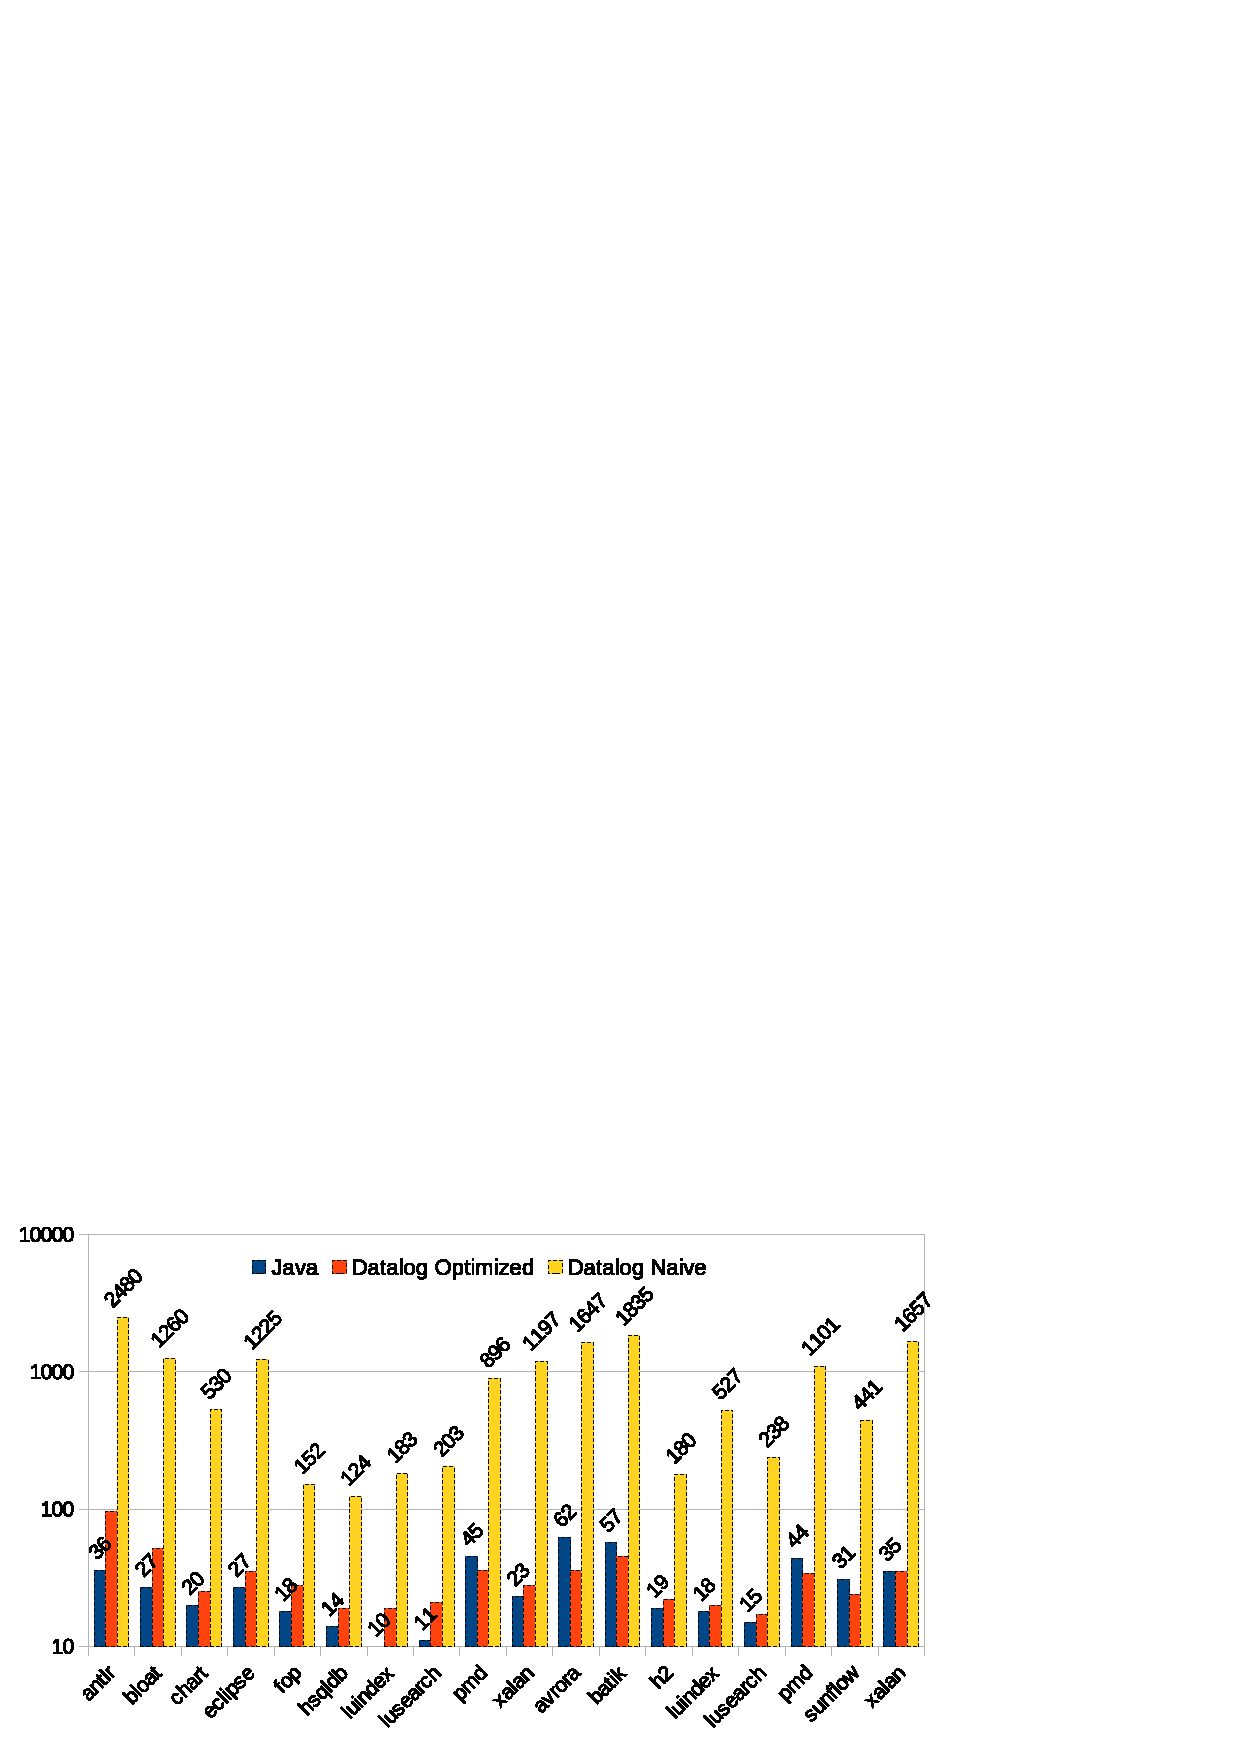
\includegraphics[width=\linewidth]{assets/defensive/time.pdf}
  \end{minipage}
  \caption{Running time (sec) of defensive analysis, with running time of
    2objH (with unsound reflection handling) shown as a
    baseline. Labels are shown for defensive analysis only to avoid
    crowding the plot.}
    \label{fig:time}
\end{figure}

%% As can be seen, 5def outperforms 2objH for
%% 16-of-22 benchmarks, one is tied, and 2objH is faster for 5 benchmarks
%% (also considering the 3 benchmarks for which either analysis timed out).

\paragraphhead{Client analysis: devirtualization.}
Our baseline analysis, 2objH, is highly precise and effective in
challenges such as devirtualizing calls (resolving virtual calls to a
single target method). On average, it can devirtualize 89.3\% of the
calls in the benchmarks studied (min: 78.5\%, max: 95.2\%). However,
these results are unsound and a compiler cannot act upon them. For
optimization clients, such as devirtualization, soundness is
essential. Using sound results, a JIT compiler can skip dynamic tests
(of the inline caching optimization) for all calls that the analysis
soundly covers.

Figure~\ref{fig:devirt1}
shows the virtual calls that defensive analysis devirtualizes, as a
percentage of those devirtualized by the unsound analysis.
\begin{figure}[tbhp]
  \begin{minipage}[b]{\linewidth}
    \centering
    % left bottom right top
    \includegraphics[width=\linewidth]{assets/defensive/devirt1.pdf}
  \end{minipage}
  \caption{Virtual call sites that are found to have receiver objects
    of a single type. These call sites can be soundly devirtualized.
    Numbers are shown as percentages of devirtualization achieved by
    unsound 2objH analysis.}
    \label{fig:devirt1}
\end{figure}

As can be
seen, defensive analysis manages to recover a large part of the
benefit of an unsound analysis (median \textbf{44.8\%} for
optimization under a context guard, \textbf{38.7\%} for unconditional,
\consname{Init} context, optimization), performing much better than
the baseline intra-procedural must-analysis (at 14.6\%). This answers
\textbf{RQ4} affirmatively: the coverage of defensive analysis translates
into real benefit for realistic clients.


\paragraphhead{Concurrency model.}
A compiler (JIT or AOT) author may (rightly) remark that the
concurrency model of Section~\ref{sec:assumptions} is not appropriate
for automatic optimizations. The Java concurrency model permits a lot
more relaxed behaviors, so the analysis is not sound for full Java as
stated. However, the benefit of defensive analysis is that it starts
from a sound basis and can add to it conservatively, only when it is
certain that soundness cannot possibly be violated. Accordingly, we
can remove the assumption that all shared data are accessed while
holding mutexes, by applying the load/store rules only when objects
trivially do not escape their allocating thread. We show the updated
numbers for the devirtualization client (now fully sound for Java!) in
Figure~\ref{fig:devirt2}. The difference in impact is minimal: \textbf{43\%} of
virtual call sites can be devirtualized conditionally, under some
context, while \textbf{36\%} can be devirtualized unconditionally. This
helps answer \textbf{RQ5}: defensive analysis can yield actionable results
for a well-known optimization, under the Java memory model, for a
large portion of realistic programs.

\begin{figure}[tbhp]
  \begin{minipage}[b]{\linewidth}
    \centering
    % left bottom right top
    \includegraphics[width=\linewidth]{assets/defensive/devirt2.pdf}
  \end{minipage}
  \caption{Virtual call sites (percentage of 2objH) that are found to
    have receiver objects of a single type. Updates
    Figure~\ref{fig:devirt1}, this time with soundness under a relaxed
    memory model.}
   \label{fig:devirt2}
\end{figure}

\paragraphhead{Points-to set sizes.}
Finally, it is interesting to quantify the precision of the defensive
analysis, for the points-to sets it covers. This precision is expected
to be high, since defensive analysis is flow- and context-sensitive,
but exact figures help put it in perspective.

Figure~\ref{fig:precision} shows average points-to set sizes for the
defensive analysis vs. the 2objH analysis. The sets (excluding null
values) are computed over variables covered by both analyses, for
non-empty defensive analysis sets and under context \consname{Init}
of the defensive analysis, i.e., unconditionally. (The numbers are for
the simplistic concurrency model, but remain unchanged to two
significant digits for the relaxed concurrency model.)

%% The first comparison
%% (first two numeric columns) is over variables that the defensive
%% analysis covers for \emph{some} context, while the second (next two
%% columns) over variables that the defensive analysis covers for context
%% \consname{Init}. Again, the use of context in a defensive analysis is
%% different, so both numbers are biased, but in opposite ways. The
%% \emph{some context} comparison may exclude valid contexts for which
%% 5def computes empty sets, making it seem more precise. Conversely, the
%% \emph{Init context} numbers exclude variables whose points-to set
%% depends on method parameters, thus downplaying the
%% %precision 
%% impact of 5def's 5-call-site sensitivity. Still, the overall picture
%% is clear: 5def is highly precise.


%% \begin{figure}[t]
%% %  \small
%% \footnotesize
%%   \centering
%%    \begin{tabular}{lrrrr|rr}
%%     \toprule
%%     Bench. & \multicolumn{4}{c|}{Avg. points-to over same vars} & \multicolumn{2}{c}{Analysis time (s)} \\
%%   \midrule
%%            & \multirow{2}{2em}{\raggedleft 2objH {\footnotesize \emph{/ins.}}} & {\raggedleft 5def} & \multirow{2}{2.5em}{\raggedleft 2objH Init ctx} & \multirow{2}{2.5em}{\raggedleft 5def Init ctx} & \multirow{2}{2em}{\raggedleft 2objH {\footnotesize \emph{/ins.}}} & {\raggedleft 5def} \\
%% & & & & & & \\
%%     \midrule
%%     \midrule
%% antlr           &  1.55	 & 	1.13    & 1.10	 & 1.01   &  382   &  858  \\  
%% bloat           &  5.45	 & 	1.86    & 2.12	 & 1.02   &  4152  &  2045 \\
%% chart           &  1.37	 & 	1.29    & 1.09	 & 1.09   &  685   &  1644 \\
%% eclipse         &  1.81	 & 	1.17    & 1.31	 & 1.06   &  483   &  652  \\
%% hsqldb          &  1.09	 & 	1.04    & 1.04	 & 1.01   &  236   &  676  \\ 
%% jFlex           &  1.41  & 	1.19    & 1.02	 & 1.01   &  965   &  398  \\
%% \emph{jython*}  &  \emph{31.08} &  2.02    & \emph{6.05}	 & 1.01   &  \emph{655}   &  1435 \\ 
%% luindex         &  1.22	 & 	1.13    & 1.02	 & 1.02   &  197   &  562  \\
%% lusearch        &  1.35	 & 	1.21    & 1.06	 & 1.04   &  210   &  579  \\
%% NTI             &  1.47	 & 	1.43    & 1.03	 & 1.03   &  189   &  102  \\
%% xalan           &  2.55	 & 	1.77    & 1.12	 & 1.05   &  440   &  1152 \\
%%     \bottomrule
%%   \end{tabular}
%%   \caption{Points-to set sizes for non-empty sets of common variables for both analyses,
%%     and running times of analyses.}
%%   \label{fig:core}
%% \end{figure}

\begin{figure}[th!p]
%  \small
\footnotesize
  \centering
  \begin{tabular}{|cl|rr|}
    \toprule
    \multirow{2}{4em}{Benchmark}  & & \multicolumn{2}{c|}{Average points-to over same vars} \\
                   &             & defensive & 2objH  \\
  \midrule
  \midrule        
\multirow{11}{-0.2cm}{\rotatebox{90}{\footnotesize{\mbox{DaCapo 2006-10-MR2}}}} 
& antlr          & 1.01   &         1.10  \\
& bloat          & 1.02   &         2.12 	 \\
& chart          & 1.09   &         1.09 	 \\
& eclipse        & 1.06   &         1.31 	 \\
& fop            & 1.00   &         1.03 	 \\
& hsqldb         & 1.01   &         1.04   \\
& jython*        & 1.01   &         6.05 	 \\
& luindex        & 1.02   &         1.02   \\
& lusearch       & 1.04   &         1.06 	 \\
& pmd            & 1.01   &         1.05 	 \\
& xalan          & 1.05   &         1.12 	 \\
\midrule
& jFlex          & 1.01   &         1.02 	 \\
& NTI            & 1.03   &         1.03     \\
\midrule        
\multirow{9}{-0.2cm}{\rotatebox{90}{\footnotesize{\mbox{DaCapo 9.12-Bach}}}}
& avrora         & 1.05   &         3.04  \\
& batik          & 1.04   &         1.05 \\
& eclipse        & 1.07   &         1.53 \\
& h2*            & 1.04   &         2.07 \\
& luindex        & 1.01   &         1.04 \\
& lusearch       & 1.03   &         1.08 \\
& pmd            & 1.01   &         1.04 \\
& sunflow        & 1.05   &         1.08 \\
& xalan\^        & 1.04   &         1.19 \\
\midrule
& \textbf{mean} &   1.03     &  1.51  \\
    \bottomrule
  \end{tabular}
  \caption{Average number of abstract objects per variable, for variables for which both
    analyses compute results.}
  \label{fig:precision}
\end{figure}

As can be seen, the defensive analysis is highly precise when it produces non-empty
points-to sets, typically yielding points-to set sizes very close to
1. 2objH is also a very precise analysis (for variables with bounded
points-to sets), so it remains competitive, yet clearly less precise.
Notably, points-to set sizes close to 1 are the Holy Grail of points-to
analysis: such precision is actionable for nearly all conceivable clients
of a points-to analysis.


%% \begin{figure}[th!p]
%% %  \small
%% \footnotesize
%%   \centering
%%   \begin{tabular}{|cl|rrrr|}
%%     \toprule
%%     \multicolumn{2}{|l|}{\multirow{4}{4em}{Benchmark}} & \multirow{4}{5.5em}{\raggedleft App. calls devirtualized, 5def {\footnotesize \emph{($\dagger$4def)}} some context} & \multirow{3}{3em}{\raggedleft \% of 2objH {\footnotesize \emph{(*ins.)}}} & \multirow{4}{5.5em}{\raggedleft App. calls devirtualized, 5def {\footnotesize \emph{($\dagger$4def)}} \\ Init context} & \multirow{3}{3em}{\raggedleft \% of 2objH {\footnotesize \emph{(*ins.)}}}   \\
%%  & & & & & \\
%%  & & & & & \\
%%  & & & & & \\
%%   \midrule
%%   \midrule        
%% \multirow{11}{-0.2cm}{\rotatebox{90}{\footnotesize{\mbox{DaCapo 2006-10-MR2}}}} 
%% & antlr          & 7974     & 46.9\%   & 5825  & 34.3\% \\
%% & bloat          & 4821     & 35.9\%   & 3954  & 29.5\%	 \\
%% & chart          & 1022     & 26.7\%   & 820   & 21.4\%	 \\
%% & eclipse        & 2525     & 44.2\%   & 2191  & 38.4\%	 \\
%% & fop            & 764      & 35.8\%   & 645   & 30.3\%	 \\
%% & hsqldb         & 586      & 59.0\%   & 545   & 54.8\%  \\
%% & \emph{jython*} & 3623     & 31.7\%   & 3147  & 27.5\%	 \\
%% & luindex        & 930      & 44.8\%   & 870   & 41.9\%  \\
%% & lusearch       & 1055     & 44.0\%   & 939   & 39.1\%	 \\
%% & pmd            & 1876     & 42.5\%   & 1689  & 38.2\%	 \\
%% & xalan          & 1653     & 21.3\%   & 1155  & 14.9\%	 \\
%% \midrule
%% & jFlex          & 1190     & 43.9\%   & 933  &  34.4\%	 \\
%% & NTI            & 481      & 50.4\%   & 381  &  39.9\%    \\
%% \midrule        
%% \multirow{9}{-0.2cm}{\rotatebox{90}{\footnotesize{\mbox{DaCapo 9.12-Bach}}}}
%% & avrora         & 4564      & 43.9\%	 & 3996 & 38.5\%  \\
%% & batik          & 4404      & 30.6\%	 & 2527 & 17.6\% \\
%% & eclipse        & 2882      & 43.5\%    & 2490 & 37.6\% \\
%% & {\em h2*}      & 8452      & 42.0\%    & 7569 & 37.6\% \\
%% & luindex        & 2010      & 46.4\%    & 1761 & 40.7\% \\
%% & lusearch       & 1614      & 50.4\%    & 1349 & 42.1\% \\
%% & pmd            & 2262      & 39.3\%    & 1986 & 34.5\% \\
%% & sunflow        & 1114      & 35.1\%    & 780  & 24.5\% \\
%% & {\em xalan$\dagger$}& 4545 & 21.4\%	 & 3554 & 16.7\% \\
%% \midrule
%% & \textbf{median} &            &   43.0\%  &        &  36.0\%  \\
%%     \bottomrule
%%   \end{tabular}
%%   \caption{Virtual calls resolved to a single target method under relaxed concurrency model.}
%%   \label{fig:client2}
%% \end{figure}

%% \begin{figure}[t]
%% %  \small
%% \footnotesize
%%   \centering
%%    \begin{tabular}{lrrrr|rr}
%%     \toprule
%%     Bench. & \multicolumn{4}{c|}{Avg. points-to over same vars} & \multicolumn{2}{c}{Analysis time (s)} \\
%%   \midrule
%%            & \multirow{2}{2em}{\raggedleft 2objH {\footnotesize \emph{/ins.}}} & {\raggedleft 5def} & \multirow{2}{2.5em}{\raggedleft 2objH Init ctx} & \multirow{2}{2.5em}{\raggedleft 5def Init ctx} & \multirow{2}{2em}{\raggedleft 2objH {\footnotesize \emph{/ins.}}} & {\raggedleft 5def} \\
%% & & & & & & \\
%%     \midrule
%%     \midrule
%% antlr           &  1.55	 & 	1.13    & 1.10	 & 1.01   &  382   &  858  \\  
%% bloat           &  5.45	 & 	1.86    & 2.12	 & 1.02   &  4152  &  2045 \\
%% chart           &  1.37	 & 	1.29    & 1.09	 & 1.09   &  685   &  1644 \\
%% eclipse         &  1.81	 & 	1.17    & 1.31	 & 1.06   &  483   &  652  \\
%% hsqldb          &  1.09	 & 	1.04    & 1.04	 & 1.01   &  236   &  676  \\ 
%% jFlex           &  1.41  & 	1.19    & 1.02	 & 1.01   &  965   &  398  \\
%% \emph{jython*}  &  \emph{31.08} &  2.02    & \emph{6.05}	 & 1.01   &  \emph{655}   &  1435 \\ 
%% luindex         &  1.22	 & 	1.13    & 1.02	 & 1.02   &  197   &  562  \\
%% lusearch        &  1.35	 & 	1.21    & 1.06	 & 1.04   &  210   &  579  \\
%% NTI             &  1.47	 & 	1.43    & 1.03	 & 1.03   &  189   &  102  \\
%% xalan           &  2.55	 & 	1.77    & 1.12	 & 1.05   &  440   &  1152 \\
%%     \bottomrule
%%   \end{tabular}
%%   \caption{Points-to set sizes for non-empty sets of common variables for both analyses,
%%     and running times of analyses.}
%%   \label{fig:core}
%% \end{figure}

%\paragraphhead{Summary.}
%%The evaluation shows the great benefits of defensive
%%analysis (speed, precision)
%Defensive analysis offers speed and precision, while covering a
%non-trivial part of the program. The devirtualization client clearly
%demonstrates practical benefit.
%%of being sound.


%\afterpage{\FloatBarrier}







\section{Conclusions}

Static analysis has long suffered from unsoundness for perfectly
realistic language features, such as reflection, native code, or
dynamic loading. We presented a new analysis architecture that
achieves soundness by being \emph{defensive}. Despite its conservative
nature, the analysis manages to yield useful results for a large
subset of the code in realistic Java programs, while being efficient
and scalable. Additionally, the analysis is modular, as it can be
applied to any subset of a program and will yield sound results.

We expect this approach to open significant avenues for further
work. The analysis architecture can serve as the basis of other sound
analysis designs. The defensive analysis itself can be combined with
several other analyses (may-escape, must-alias) that have so far been
hindered by the lack of a sound substrate.
%The analysis can be enhanced with a wealth of
%extra information to extend its coverage.


%% \begin{figure*}[t]
%%   \small
%%   \centering
%%   \begin{tabular}{lrrrrrrrrrrrr}
%%     \toprule
%%     \multicolumn{13}{c}{\large \emph{Alias pairs}} \\
%%     % \cmidrule(l){2-13}
%%     \midrule
%%     & \multicolumn{3}{c}{intra-procedural}
%%     & \multicolumn{3}{c}{intra-procedural$^{+\text{may}}$}
%%     & \multicolumn{3}{c}{inter-procedural$_{-\text{may}}$}
%%     & \multicolumn{3}{c}{inter-procedural} \\
%%     \cmidrule(lr){2-4} \cmidrule(lr){5-7} \cmidrule(lr){8-10} \cmidrule(l){11-13}
%%     & \multirow{2}{2em}{per instr.} & \multirow{2}{3em}{\hfill per all-return} & time
%%     & \multirow{2}{2em}{per instr.} & \multirow{2}{3em}{per all-return} & time
%%     & \multirow{2}{2em}{per instr.} & \multirow{2}{3em}{per all-return} & time
%%     & \multirow{2}{2em}{per instr.} & \multirow{2}{3em}{per all-return} & time
%%     \\ Benchmark \\
%%     \midrule
%%     antlr    &  7 &  3 & 5m18s & 41 &  6 &  7m2s &  34 & 19 &  18m6s & 105 & 27 & 41m18s \\
%%     chart    & 10 &  4 & 5m58s & 15 &  6 & 5m55s &  26 & 20 &  7m52s & 34 & 24 &  9m18s \\
%%     luindex  &  4 &  3 & 2m27s &  7 &  6 & 2m50s &   7 &  7 &  3m17s & 12 & 12 &  3m25s \\
%%     lusearch &  5 &  3 & 2m51s &  6 &  5 & 2m52s &   8 &  6 &  3m20s & 12 & 10 &  3m54s \\
%%     pmd      & 13 &  3 & 5m44s & 15 &  4 & 5m37s &  23 & 17 & 11m17s & 27 & 19 & 12m57s \\
%%     \bottomrule
%%   \end{tabular}
%%   \caption{Average \#alias pairs per program element (with equivalent
%%     symmetric pairs removed, i.e., numbers divided by 2), and timings
%%     for various settings of the must-alias analysis.}
%%   \label{fig:exp1}
%% \end{figure*}



%\clearpage

%\renewcommand{\baselinestretch}{0.89}
%\renewcommand{\parsep}{0.2em}
%\bibliographystyle{super-abbrv}

%\bibliographystyle{abbrvnat}% \renewcommand{\bibfont}{\normalsize}
% \bibliography{cumulative-bib}

%%% Supplementary
%\begin{comment}


%% \appendix

%% \section{Soundness Proof}

%% We present informal but rigorous proofs of the main claims of our
%% analysis.

%% \subsection{Assumption/Guarantee Lemma}

%% We next discuss rules incrementally, with an eye towards establishing
%% their soundness. For each rule, we will present the soundness
%% \emph{assumptions} (preconditions) and \emph{guarantees}
%% (postconditions) it offers. We will later appeal to these properties
%% as a lemma in our soundness proof.

%% \paragraphhead{Initializing the analysis.}
%% The first rule initializes the analysis by making all
%% root methods reachable.

%% \begin{rules}
%% \rel{Reachable}{\consname{All}, meth} \rulearrow{} \relConf{RootMethod}{meth}.\\
%% \end{rules}

%% There are no soundness assumptions or guarantees for the above
%% rule. The input relation \relname{RootMethod} can contain arbitrary
%% contents and only affects the coverage of the analysis (since
%% otherwise points-to sets remain empty, i.e., implicitly
%% over-approximate).

%% \paragraphhead{Object allocation.} The 
%% handling of \relname{Alloc} instructions provides an unconditionally
%% sound points-to set. It is a base case for our inductive reasoning.

%% \begin{rules}
%% \rel{PointsTo}{i, ctx, \consapp{AP}{var}, heap} \rulearrow{} \\
%% \tab \rel{Alloc}{i, var, heap}, \rel{InMethod}{i, meth}, \\
%% \tab \rel{Reachable}{ctx, meth}. \\
%% \end{rules}

%% The rule computes an over-approximation of points-to sets \emph{per
%%   allocation instruction and its local variable}. (Other points-to
%% sets at the same program point---e.g., points-to sets carried over
%% from previous instructions---are not the responsibility of this rule,
%% so establishing their soundness is part of later reasoning.)

%% \myparagraph{Assumption:} the rule makes no assumptions on the state
%% of the computation before its firing.
%% % (Unlike later rules.) 

%% \myparagraph{Guarantee:} the rule produces over-approximate points-to
%% sets for all variables, \args{var}, that match in an execution of the
%% rule. This is easy to establish: at first, all points-to sets of such
%% \args{var}s are empty, i.e., denoting an implicitly over-approximate
%% value of $\top$. Once the rule executes and its body matches for a
%% certain allocation instruction \args{i}, the points-to set of the
%% variable assigned at \args{i} can only contain the freshly-allocated
%% object, \args{heap}, which is what the rule computes. No other program
%% instruction, in known or opaque code, can affect this
%% inference.\footnote{Recall that we assume an isolated heap and
%%   stack frames: no external code can affect local variables. We will
%%   use this assumption implicitly throughout.}

%% %\footnote{Recall our earlier warning about concurrency
%% %  models: we assume that all shared data accesses are
%% %  mutex-protected, so that no other thread can interfere with the
%% %  assignment. In Java-like languages, without an address-of operator
%% %  for local variables (such as the C/C++ \texttt{\&}), even this
%% %  assumption is unnecessary for this rule: local variable \args{var}
%% %  is guaranteed thread-local.}


%% \paragraphhead{Variable moves.} \relname{Move} instructions
%% can only produce sound sets if their input is sound.

%% \begin{rules}
%% \rel{PointsTo}{i, ctx, toAp, heap} \rulearrow{} \\
%% \tab \rel{Move}{i, to, from}, \\
%% \tab \rel{Before:PointsTo}{i, ctx, fromAp, heap}, \\
%% \tab \func{RebaseAP}{fromAp, from, to}{toAp}.\\
%% \end{rules}

%% \myparagraph{Assumption:} before execution of the rule, the points-to
%% set encoded in relation \relname{Before:PointsTo} (more precisely:
%% for every triple \args{i,ctx,fromAp} that matches the rule body in the
%% rule execution) is sound, i.e., it is either empty (to signify $\top$)
%% or contains all possible values that the access path may point to at
%% the given instruction and for any dynamic context matching the
%% analysis context. (In subsequent discussion we shall be less pedantic
%% in defining the points-to sets and values in question, since these are
%% easy to deduce in the context of a rule's explanation.)

%% \myparagraph{Guarantee:} The resulting points-to sets (encoded in
%% relation \relname{PointsTo}, for any \args{(i,ctx,toAp)} that match
%% in an execution of the rule) are sound, \emph{after full execution of
%%   the rule}. The latter is a subtle point, worth emphasizing, since it
%% is pervasive in our soundness reasoning.  Datalog rules induce
%% point-wise inferences. Our above rule refers to a single object,
%% \args{heap}, at a time, and not to the entire points-to set of
%% \args{fromAp} at once. Therefore, the rule's guarantee of soundness
%% only holds after the rule has been applied over the entire contents of
%% the relations in its body and all possible inferences have been
%% made. It is entirely possible that, during intermediate stages of the
%% rule's evaluation, points-to sets will be incomplete, i.e., neither
%% empty, nor containing all possible values. After full evaluation,
%% however, the soundness of the rule (under its earlier ``assumption''
%% on the input) is self-evident.


%% \paragraphhead{Heap loads.} Similarly, heap loads produce over-approximate
%% points-to sets if their input is also over-approximate.

%% \begin{rules}
%% \rel{PointsTo}{i, ctx, \consapp{AP}{to}, heap} \rulearrow{} \\
%% \tab \rel{Load}{i, to, base, fld}, \\
%% \tab \rel{Before:PointsTo}{i, ctx, \consapp{AP}{base.fld}, heap}.\\
%% \end{rules}

%% \myparagraph{Assumption:} As in the previous rule, before execution of
%% the rule, the points-to set encoded in relation
%% \relname{Before:PointsTo} should be sound (over-approximate), i.e.,
%% it is either empty or contains all possible values that an access path
%% may point to.

%% \myparagraph{Guarantee:} As before, the resulting points-to sets are
%% sound, after full execution of the rule (modulo concurrency models---recall
%% that we assume mutex-protected access to all shared data throughout).


%% \paragraphhead{Heap stores.} The next two rules handle writes to the heap
%% (store instructions).

%% \begin{rules}
%% \rel{PointsTo}{i, ctx, \consapp{AP}{base.fld}, heap} \rulearrow{} \\
%% \tab \rel{Store}{i, base, fld, from}, \\
%% \tab \rel{Before:PointsTo}{i, ctx, \consapp{AP}{from}, heap}.\\
%% \\
%% \rel{PointsTo}{i, ctx, ap, heap1},\\
%% \rel{PointsTo}{i, ctx, ap, heap2} \rulearrow{} \\
%% \tab \rel{Store}{i, base, fld, from}, \\
%% \tab \rel{Before:PointsTo}{i, ctx, \consapp{AP}{from}, heap1},\\
%% \tab \rel{Before:PointsTo}{i, ctx, ap, heap2},\\
%% \tab \args{ap} = \consapp{AP}{base'.fld}, \args{base} $\neq$ \args{base'}.\\
%% \end{rules}

%% \myparagraph{Assumption:} Before execution of the rule, the points-to
%% sets encoded in relation \relname{Before:PointsTo}, for any of the
%% involved access paths, should be sound (i.e., over-approximate).

%% \myparagraph{Guarantee:} As before, the resulting points-to sets are
%% sound, after full execution of the rule (modulo concurrency models).
%% To see this, consider that the second rule takes the union of the two
%% points-to sets (of \args{from} and of \args{ap}, both before the
%% instruction) as long as neither set is empty. At a store instruction,
%% there is nothing that can influence the contents of an object field,
%% other than its previous contents and the currently assigned value,
%% hence the rule is fully conservative.


%% \paragraphhead{Control-flow predecessors.} 
%% Next comes the rule for merging information from an instruction's
%% predecessors.

%% \begin{rules}
%% \rel{Before:PointsTo}{i, ctx, ap, heap} \rulearrow{} \\
%% \tab \rel{Next}{pred, i}, \\
%% \tab \rel{PointsTo}{pred, ctx, ap, heap},\\
%% \tab ($\forall$\args{j}: \rel{Next}{j, i} \ruleforall{} \rel{PointsTo}{j, ctx, ap, \_}).\\
%% \end{rules}

%% \myparagraph{Assumption:} Before execution of the rule, the points-to
%% sets encoded in relation \relname{PointsTo} should be sound, i.e.,
%% for each predecessor, the points-to set of \args{ap} at that
%% predecessor is either empty or contains all possible values that the
%% access path may point to.

%% \myparagraph{Guarantee:} The resulting points-to set is sound
%% (over-approximate), after full execution of the rule. This is easy to
%% establish by considering that the rule takes the union of all input
%% points-to sets (\relname{PointsTo} for \args{ap} at all predecessors)
%% as long as no single one of them is empty.
%% % (If even a single input
%% %points-to set for \args{ap} is empty, the rule does not match, hence
%% %the resulting points-to set is also empty, and not the union, as
%% %discussed in Section~\ref{sec:illustration}.)


%% \paragraphhead{Frame rules: before an instruction to after it.}
%% The next three rules state the
%% conditions under which points-to information can be kept unchanged by
%% an instruction.

%% \begin{rules}
%% \rel{PointsTo}{i, ctx, ap, heap} \rulearrow{} \\
%% \tab \rel{Before:PointsTo}{i, ctx, ap, heap}, \args{ap} = \consapp{AP}{var}, \\
%% \tab !\rel{Load}{i, var, \_, \_}, !\rel{Move}{i, var, \_}, \\
%% \tab !\rel{Alloc}{i, var, \_}, !\rel{Unknown}{i}.\\
%% \\
%% \rel{PointsTo}{i, ctx, ap, heap} \rulearrow{} \\
%% \tab \rel{Before:PointsTo}{i, ctx, ap, heap}, \args{ap} = \consapp{AP}{var.\_}, \\
%% \tab !\rel{Call}{i, \_, \_}, !\rel{Store}{i, \_, \_, \_}, !\rel{Load}{i, var, \_, \_}, \\
%% \tab !\rel{Move}{i, var, \_}, !\rel{Alloc}{i, var, \_}, !\rel{Unknown}{i}.\\

%% \\
%% \rel{PointsTo}{i, ctx, ap, heap} \rulearrow{} \\
%% \tab \rel{Store}{i, \_, fld, \_}, \\
%% \tab \rel{Before:PointsTo}{i, ctx, ap, heap}, \\
%% \tab \args{ap} = \consapp{AP}{\_.\_}, \args{ap} $\neq$ \consapp{AP}{\_.fld.\_}. \\
%% \end{rules}

%% \myparagraph{Assumption:} Before execution of each rule, the points-to
%% set for \args{ap} encoded in relation \relname{Before:PointsTo}
%% should be sound (over-approximate).

%% \myparagraph{Guarantee:} For each rule separately, the resulting
%% points-to set (in relation \relname{PointsTo}) is sound after full
%% execution of the rule. This requires some care to establish. First,
%% note that in our limited intermediate language (of 7 instructions
%% only) no instruction kind assigns a local variable, other than
%% \relname{Alloc}, \relname{Move} or \relname{Load}. (\relname{Call}
%% instructions cannot alter the value of local variables in their
%% callee, assuming call-by-value semantics and no pointers to local
%% variables, as discussed earlier.) Second, consider that the treatment
%% of \relname{Unknown} instructions is as conservative as it can
%% possibly be: all points-to information is dropped when an unknown
%% instruction is encountered. Finally, a potential complication arises
%% in that the applicability of these rules may overlap with the
%% applicability of earlier rules (or with each other). Inspection of all
%% cases (e.g., consider the above three rules and the two rules handling
%% heap store instructions) reveals that the body conditions of each frame
%% rule are mutually exclusive with the body conditions of earlier
%% rules or other frame rules.  

%% Therefore, a frame rule will either not be triggered, in which case
%% its output points-to set is empty (i.e., trivially over-approximate),
%% or will compute points-to sets for an access path \args{ap} after an
%% instruction \args{i}, such that \args{i} cannot have altered the points-to
%% set of \args{ap}. In the latter case, the (assumed over-approximate) points-to
%% set of \args{ap} from before the instruction is maintained and is, thus,
%% also over-approximate. 

%% The latter holds, again, modulo a concurrency model. Importantly,
%% our assumed model throughout this paper (shared data only accessed
%% while holding mutexes) is trivially handled by the above rules: a
%% mutex acquire instruction (e.g., a JVM \code{monitorenter}) is not
%% captured in our language, hence it is encoded as an ``unknown''
%% instruction.  Per the frame rules, this ensures that all points-to
%% information is prevented from propagating over a possible point of
%% interference from other threads.


%% \paragraphhead{Inter-procedural analysis: Over-approximate call-graph.}
%% Our next rule uses points-to information to establish a sound call-graph.

%% \begin{rules}
%% \rel{CallGraphEdge}{i, ctx, toMeth, toCtx}, \\
%% \rel{Reachable}{toCtx, toMeth} \rulearrow{} \\
%% \tab \rel{Call}{i, base, sig}, \\
%% \tab \rel{Before:PointsTo}{i, ctx, \consapp{AP}{base}, heap}, \\
%% \tab \rel{HeapType}{heap, type}, \rel{LookUp}{type, sig, toMeth}, \\
%% \tab \func{NewContext}{i, ctx, heap}{toCtx}.\\
%% \end{rules}

%% \myparagraph{Assumption:} Before execution of the rule, the points-to
%% set for \args{base} encoded in relation \relname{Before:PointsTo}
%% should be sound (over-approximate).

%% \myparagraph{Guarantee:} Relation \relname{CallGraphEdge} for
%% invocation site \args{i} encodes a sound call-graph for instruction
%% \args{i} under context \args{ctx}. Since \relname{Before:PointsTo}
%% over-approximates the receiver object for \args{(i,ctx)}, we also
%% derive (via type system lookup) an over-approximation of
%% the call targets (including empty as a trivial over-approximation).


%% \paragraphhead{Inter-procedural propagation of values: caller-to-callee.}

%% The next rule handles points-to information propagation over calls,
%% from caller to callee.

%% \begin{rules}
%% \rel{Before:PointsTo}{fstInstr, toCtx, ap, heap} \rulearrow{} \\
%% \tab \rel{CallGraphEdge}{i, ctx, toMeth, toCtx}, \\
%% \tab \rel{InMethod}{fstInstr, toMeth}, 
%%      ($\forall$\args{k}: \ruleforall{} !\rel{Next}{k, fstInstr}), \\
%% \tab \rel{Before:PointsTo}{i, ctx, callerAp, heap}, \\
%% \tab \rel{FormalArg}{toMeth, n, toVar}, \rel{ActualArg}{i, n, var}, \\
%% \tab \func{RebaseAP}{callerAp, var, toVar}{ap}.\\
%% \end{rules}

%% \myparagraph{Assumption:} Before execution of the rule, the points-to
%% sets encoded in relation \relname{Before:PointsTo} (for \args{base},
%% under \args{(i,ctx)} matching in the rule body) are over-approximate.

%% \myparagraph{Guarantee:} The points-to set computed (for \args{ap} at
%% instruction \args{fsInstr} under context \args{toCtx}) is
%% over-approximate, \emph{as long as the pair \args{(toMeth,toCtx)}
%%   uniquely identifies \args{i} and \args{ctx}}!  The latter is an
%% important restriction on the possible definitions of function
%% \consname{NewContext}. Rigorously speaking, we are trying to establish
%% that the set of \args{heap} values in \rel{Before:PointsTo}{fstInstr,
%%   toCtx, ap, heap} is over-approximate, given that
%% \rel{Before:PointsTo}{i, ctx, callerAp, heap} is. Values of variable
%% \args{fstInstr} map one-to-one to values of \args{toMeth}, and (given
%% invocation site \args{i} and target method \args{toMeth}) \args{ap}
%% maps one-to-one to \args{callerAp}. Hence, if the pair
%% \args{(toMeth,toCtx)} arises for only a single call site and caller
%% context pair, \args{(i,ctx)}, then the property clearly holds.  Recall
%% that this is our requirement for constructor \consname{NewContext}: it
%% should at least encode call-site sensitivity, i.e., the callee context
%% has to uniquely identify the call site.


%% \paragraphhead{Inter-procedural propagation of values: callee-to-caller.}
%% The next two rules perform a similar propagation of values, this time
%% from callee to caller. 
%% %A subtle difference from earlier is that the
%% %rule is predicated on having computed an over-approximation of the
%% %targets of a virtual call in relation \relname{CallGraphEdge}.
%% %(We
%% %did not need this assumption for propagation of points-to sets from
%% %caller to callee precisely because this information was predicated on
%% %context that uniquely identified the caller.)

%% \begin{rules}
%% \rel{RebaseAPForReturn}{i, ap, newAp} \rulearrow{} \\
%% \tab \rel{CallGraphEdge}{i, \_, toMeth, \_}, \\
%% \tab \rel{FormalArg}{toMeth, n, var}, \rel{ActualArg}{i, n, toVar}, \\
%% \tab \args{ap} = \consapp{AP}{\_.\_}, \func{RebaseAP}{ap, var, toVar}{newAp}.\\
%% \\
%% \rel{PointsTo}{i, ctx, ap, heap} \rulearrow{} \\
%% \tab \rel{CallGraphEdge}{i, ctx, toMeth, toCtx}, \\
%% \tab \rel{Return}{ret}, \rel{InMethod}{ret, toMeth}, \\
%% \tab \rel{Before:PointsTo}{ret, toCtx, calleeAp, heap}, \\
%% \tab \rel{RebaseAPForReturn}{i, calleeAp, ap}, \\
%% \tab ($\forall$\args{toMeth'}, \args{toCtx'}: \\
%% \tab \tab \rel{CallGraphEdge}{i, ctx, toMeth', toCtx'} \ruleforall{} \\
%% \tab \tab ($\exists$\args{ret'}, \args{calleeAp'}: \\
%% \tab \tab \tab \rel{Return}{ret'}, \rel{InMethod}{ret',toMeth'},  \\
%% \tab \tab \tab \rel{Before:PointsTo}{ret', toCtx', calleeAp', \_}, \\
%% \tab \tab \tab \rel{RebaseAPForReturn}{i, calleeAp', ap})). \\
%% \end{rules}

%% \myparagraph{Assumption:} Before execution of the rule, the points-to
%% sets encoded in relation \relname{Before:PointsTo} as well as the
%% call-graph encoded in \relname{CallGraphEdge} are
%% over-approximate.
%% %\footnote{Interestingly, we did not need the assumption
%% %that \relname{CallGraphEdge} be over-approximate for the case of
%% %propagating information from caller to callee, but we do for propagating
%% %information back from callee to caller. Intuitively, this continues our
%% %earlier remarks on how a defensive analysis only establishes points-to
%% %information at a callee conditionally, under a specific context that
%% %identifies the caller.}

%% \myparagraph{Guarantee:} The points-to set computed (for \args{ap} at
%% call-site \args{i}) is over-approximate. As in the case of store
%% instructions and control-flow merge points, the rule takes the union
%% of points-to sets for \args{ap} (suitably renamed) at all return
%% points (``all'' established by the soundness of
%% \relname{CallGraphEdge}), as long as not a single one of them is
%% empty. If any such points-to set is empty, the rule fails to match at
%% all, hence the overall resulting points-to set is empty.

%% It is worth noting that the handling of a method return is the only
%% point where a context can become stronger. Facts that were inferred to
%% hold under the more specific \args{toCtx} are now established, modulo
%% rebasing, under \args{ctx}.








%% \paragraphhead{Summary.}
%% This concludes the analysis model for our core intermediate language.
%% (There are many elements that can be added to the analysis to make it
%% more suitable for full languages and realistic programs. We postpone
%% the discussion of enhancements until Section~\ref{sec:discussion}.)  The
%% essence of the analysis is well-captured by this model. It is also
%% evident that the analysis has a strikingly different form from past
%% (unsound) points-to analyses in the literature. At every key point
%% (notably: control-flow merging, heap stores, inter-procedural
%% propagation of points-to sets) the analysis defensively ensures that
%% the information it has available is sufficient to establish an
%% upper-bounded points-to set, otherwise it reverts to computing an
%% empty set.




%% Reachable(ALL, meth) <-
%%    RootMethod(meth).

%% PointsTo(i, ctx, AP(var), heap) <-
%%    Alloc(i, var, heap),
%%    InMethod(i, meth),
%%    Reachable(ctx, meth).

%% PointsTo(i, ctx, toAp, heap) <-
%%    Move(i, to, from),
%%    Before:PointsTo(i, ctx, fromAp, heap),
%%    RebaseAP(fromAp, from, to) = toAp.

%% %PointsTo(i, ctx, toAp, heap) <-
%% %   Phi(i, _, _, ...),
%% %   (forall from: Phi(i, to, ..., from, ...) ->
%% %     Before:PointsTo(i, ctx, RebaseAP(toAp, to, from), heap)).

%% NewContext(i, ctx, heap) = toCtx,
%% CallGraphEdge(i, ctx, toMeth, toCtx),
%% Reachable(toCtx, toMeth) <-
%%    Call(i, base, sig),
%%    Before:PointsTo(i, ctx, AP(base), heap),
%%    HeapType(heap, type),
%%    LookUp(type, sig, toMeth).

%% ===============================

%% PointsTo(i, ctx, AP(to), heap) <-
%%    Load(i, to, base, fld),
%%    Before:PointsTo(i, ctx, AP(base.fld), heap).

%% PointsTo(i, ctx, AP(base.fld), heap) <-
%%    Store(i, base, fld, from),
%%    Before:PointsTo(i, ctx, AP(from), heap).

%% PointsTo(i, ctx, ap, heap1),
%% PointsTo(i, ctx, ap, heap2) <-
%%    Store(i, base, fld, from),
%%    Before:PointsTo(i, ctx, AP(from), heap1),
%%    Before:PointsTo(i, ctx, ap, heap2),
%%    ap = AP(base2.fld),
%%    base != base2.

%% %===============================
%% %// weakening
%% %
%% %PointsTo(i, ctx, ap, heap) <-
%% %   InMethod(i, meth),
%% %   Reachable(ctx, meth),
%% %   PointsTo(i, ALL, ap, heap).
%% %
%% %Before:PointsTo(i, ctx, ap, heap) <-
%% %   InMethod(i, meth),
%% %   Reachable(ctx, meth),
%% %   Before:PointsTo(i, ALL, ap, heap).
%% %
%% %===============================

%% // frame rules

%% Before:PointsTo(i, ctx, ap, heap) <-
%%    Next(pred, i), 
%%    PointsTo(pred, ctx, ap, heap),
%%    (forall j: Next(j, i) ->
%%       PointsTo(j, ctx, ap, _)).

%% PointsTo(i, ctx, ap, heap) <-
%%    Before:PointsTo(i, ctx, ap, heap),
%%    ap = AP(var),
%%    !Load(i, var, _, _),
%%    !Move(i, var, _),
%%    !Alloc(i, var, _),
%%    !Unknown(i).

%% PointsTo(i, ctx, ap, heap) <-
%%    Before:PointsTo(i, ctx, ap, heap),
%%    ap = AP(var._),
%%    !Call(i, _, _),
%%    !Store(i, _, _, _),
%%    !Unknown(i),
%%    !Load(i, var, _, _),
%%    !Move(i, var, _),
%%    !Alloc(i, var, _).

%% PointsTo(i, ctx, ap, heap) <-
%%    Before:PointsTo(i, ctx, ap, heap),
%%    ap = AP(_._),
%%    Store(i, _, fld, _),
%%    ap != AP(_.fld._).

%% ===============================

%% Before:PointsTo(firstInstr, toCtx, ap, heap) <-
%%    CallGraphEdge(i, ctx, toMeth, toCtx),
%%    InMethod(firstInstr, toMeth), (forall k -> !Next(k, firstInstr)),
%%    Before:PointsTo(i, ctx, callerAp, heap),
%%    FormalArg(toMeth, n, toVar), ActualArg(i, n, var),
%%    RebaseAP(callerAp, var, toVar) = ap.

%% RebaseAPForReturn(i, ap, newAp) <-
%%    CallGraphEdge(i, _, toMeth, _),
%%    FormalArg(toMeth, n, var), ActualArg(i, n, toVar), AP(_.fld) = ap,
%%    RebaseAP(ap, var, toVar) = newAp.

%% PointsTo(i, ctx, ap, heap) <-
%%    CallGraphEdge(i, ctx, toMeth, toCtx),
%%    Return(ret), InMethod(ret, toMeth), 
%%    Before:PointsTo(ret, toCtx, calleeAp, heap),
%%    RebaseAPForReturn(i, calleeAp, ap),
%%    (forall toMeth', toCtx' : CallGraphEdge(i, ctx, toMeth', toCtx') ->
%%       exist ret', calleeAp':
%%         Return(ret'), InMethod(ret', toMeth'),
%%         Before:PointsTo(ret', toCtx', calleeAp', _),
%%         RebaseAPForReturn(i, calleeAp', ap)).





%\end{comment}
%% Supplementary







\begin{comment}
\section{Why Is Sound Analysis Hard?}

In a recent article \cite{article:2015:Livshits}, Livshits et al. observe that
``\textit{[there is not] a single realistic whole-program analysis
  tool [...]  that does not purposely make unsound choices
  ... [V]irtually all published whole-program analyses are unsound and
  omit conservative handling of common language features when applied
  to real programming languages}''. 
%The sentiment echoes past
%observations, in more specific settings. For instance, Avots et
%al. \cite{icse/AvotsDLL05} remark: ``\textit{A C pointer alias
%  analysis cannot be strictly sound, or else it would conclude that
%  most locations in memory may point to any memory location.}''

Our defensive analysis addresses the above problems: the
analysis is sound as-specified (regardless of the extra features of
realistic programming languages) and yields realistic benefit. To
appreciate how the different architecture of our analysis solves the
problem, we need to first examine \emph{why} past analyses did not
manage to (or chose not to) be sound. (Our discussion focuses on
may-point-to analyses, but largely applies, with small adaptation, to
other static analyses.)

\paragraphhead{Observation: implicit over-approximation.}
A simple observation regarding a sound may-point-to analysis is that
points-to sets can only be \emph{implicitly} over-approximate. I.e.,
they cannot list exhaustively all the abstract objects that a variable
can point to, but instead should have catch-all values (such as
$\top$, as in traditional data-flow analysis) or marks (such as ``I''
for ``incomplete'' in past work \cite{pldi:2007:Lattner}).

To see this, consider the traditional explicit representation of
points-to sets in a static analysis. A set \code{\{o1, o3, o17\}}
includes abstract objects \code{o1}, \code{o3}, \code{o17}, which are
typically context-qualified allocation sites, i.e., program
instructions with some extra annotations. However, this representation
cannot capture objects allocated in \emph{unknown} code, such as
dynamically loaded code. 

Therefore a sound analysis (which needs to be over-approximate, i.e.,
to capture \emph{all} objects that a variable may point to during
\emph{any} execution) has to encode unknown objects implicitly, using
a special value.
%\footnote{Of course, an analysis can be sound by
%  computing an unknown, $\top$, value \emph{everywhere}, but such an
%  analysis will be obviously useless in practice.}  
Our defensive analysis also follows this pattern, yet the value
denoting that a points-to set is not completely known is
(unconventionally, but highly conveniently) the empty set.


\paragraphhead{Difficulty: non-monotonicity.} The first practical
difficulty of having a sound points-to analysis is the logical
non-monotonicity of inter-procedural (mainly heap-related) analysis
reasoning. To see the issue, consider the treatment of a standard
``load'' instruction from a heap object:

\vspace{-3mm}\begin{minipage}[l]{5.1in}
\begin{javacodeNoLines}
x = y.fld;
\end{javacodeNoLines}
\end{minipage}

\noindent For the analysis to upper-bound the set of values that
\code{x} may point to, it does not suffice to have upper-bounded the set
of values that \code{y} may point to and the values that \code{y}'s fields
may point to. Instead, it is necessary to know that \emph{every value
  pointed-to by \code{y} does not escape into opaque code}. For
instance, one possible value of \code{y} may be aliased, e.g., it may
also be known as \code{r.next.parent}, where \code{r} is a variable used
as a parameter to an opaque operation.  Thus, \code{x} can potentially
point to anything.

The above reasoning introduces a logical conundrum:

\begin{itemize}
\item To define a sound may-point-to analysis, we first need to have
  completed a sound \emph{may-escape} analysis, and take the
  complement of its results, in order to know what objects can \emph{never}
  escape into opaque code.
\item But, to define a sound (i.e., over-approximate) may-escape
  analysis, we first need to have a sound may-point-to analysis.
\end{itemize}

The above difficulty can be overcome, by introducing highly
conservative over-approximations of either a points-to or an escape
analysis, computing the other analysis based on the conservative
estimate, refining it, etc. In practice, this is a technical
complication. More importantly, it also implies that a large number of
objects can never be proven to not escape into opaque code. Listing
all such objects explicitly would be highly inefficient.\footnote{The
  only past analysis that attempts to do so is that of Lattner et
  al. \cite{pldi:2007:Lattner}, which has a special form that sidesteps the
  inefficiency at the expense of imprecision. The analysis employs a
  Steensgaard/unification-based analysis
  model~\cite{popl:1996:Steensgaard}. In this model, no
  object can belong in more than one points-to set, thus enabling a
  highly efficient representation of large sets of objects (using
  union-find trees), which cannot, however, be distinguished.} Note
that this also means that the special implicit object values discussed
earlier (such as $\top$) will necessarily represent not just
``unknown'' objects (i.e., in not-yet-loaded code) but also perfectly
normal objects that happen to escape into opaque code.
%This observation will come back to hurt us later.


\paragraphhead{Difficulty: capturing all opaque entry points and their
behavior.} Another difficulty of producing a sound analysis is
encoding all possible entry points into opaque code and their possible
behaviors. There are thousands of entry points into opaque code in a
realistic library (e.g., in the JDK). These include all native
methods, all reflection operations, \code{invokedynamic} instructions,
and more.  Furthermore, it is hard to model all behavior of these
entry points.  A single reflection operation can result in the leaking
of a large number of objects to a completely unforeseen method. Even
modeling reflection unsoundly (but with enough effort to have a
realistic treatment) faces a heavy engineering burden. For instance,
the latest reflection handling in the \textsc{Doop}
framework~\cite{aplas:2015:Smaragdakis} spans hundreds of logical
rules---a significant portion of the overall code base.

Even worse, the analysis needs to also model dynamically loaded code,
i.e., code that may not even exist at analysis time. It is far from
trivial to consider how dynamic loading can affect the analyzed
code---no past work has done so (except in very specific client
settings~\cite{pldi:2000:Sreedhar}---see
Section~\ref{sec:related}). The reason, again, has to do with
inter-procedural interactions. Extra code has the potential of
affecting nearly every inference of a whole-program analysis (e.g.,
static variables can almost always receive new values). It is easier
to compute what (and where) \emph{cannot} be influenced by
dynamically loaded code (i.e., to be defensive), than what \emph{can}.


\paragraphhead{Difficulty: wasting most work.} A sound points-to analysis
will likely be prohibitively expensive, due to the unpredictable order
of discovering what objects can be affected by opaque code.  Consider
our earlier example of a heap load, augmented with a virtual call,
inside a loop:
% and a back-edge in the control-flow:

\vspace{-3mm}\begin{minipage}[l]{5.1in}
\begin{javacode}
while (...) {
  x = y.fld;
  x.foo(y);
}
\end{javacode}
\end{minipage}

The analysis may well soundly compute all the object values that
\code{y} may point to at the load instruction (line 2). It may also have
computed the objects that \code{y.fld} object fields may point to. One
of these computed objects may induce a different resolution of the
call instruction (line 3), which can suddenly lead to the discovery
that a \code{y.fld}-aliased object can enter opaque code (while this was
not true based on what the analysis had computed earlier)! Since the
object referenced by \code{y.fld} can change in code that is not
analyzed, the points-to set of \code{x} at the load instruction will
need to be augmented with our implicit over-approximation special
value, $\top$.  This means that all previously computed values for the
points-to sets of \code{x} and \code{y.fld} are subsumed by the single
$\top$ value (which, recall, also represents regular objects that
escape into opaque code). Computing these values and all others that
depend on them constitutes wasted effort. To make matters worse, this
is more likely to happen for \emph{large} points-to sets, i.e., the
more work the analysis has performed on computing an explicit
points-to set, the larger (and less precise) the set will be, and the more
likely it is that the work will be wasted because the set will revert
to $\top$.

\end{comment}


\part{Epilogue}
\chapter{paNda: a Datalog compiler}\label{chapter:panda}
\chapter{Related Work}
\label{chapter:related}
\epigraph{Hermits United. We meet up every 10 years, swap stories about caves. It’s good fun… for a hermit.}{\textit{The 10th Doctor} - Doctor Who}

%This chapter includes related work of previous chapters (Chapter~\ref{chapter:hybrid}-\ref{chapter:defensive}).

\section{Hybrid Context-Sensitivity}

We have discussed directly related work throughout Chapter~\ref{chapter:hybrid}. Here we selectively mention a few techniques that, although not directly related to ours, offer alternative approaches to sweet spots in the precision/performance tradeoff.

Special-purpose combinations of context-sensitivity have been used in the past, but have required manual identification of classes to be treated separately (e.g., Java collection classes, or library factory methods). An excellent representative is the TAJ work for taint analysis of Java web applications \cite{pldi:2009:Tripp}. In contrast, we have sought to map the space and identify interesting hybrids for general application of context-sensitivity, over the entire program.

The analyses we examined are context-sensitive but flow-insensitive. We can achieve several of the benefits of flow-sensitivity by applying the analysis on the static single assignment (SSA) intermediate form of the program. This is easy to do with a mere flag setting on the \doop{} framework. However, the impact of the SSA transformation on the input is minimal. The default intermediate language used as input in \doop{} (the Jimple representation of the Soot framework \cite{cascon:1999:Vall,cc:2000:Vall}) is already close to SSA form, although it does not guarantee that every variable is strictly single-assignment without requesting it explicitly. Published work by Lhot\'{a}k and Chung \cite{popl:2011:Lhotak} has shown that much of the benefit of flow-sensitivity derives from the ability to do strong updates of the points-to information. Lhot\'{a}k and Chung then exploited this insight to derive analyses with similar benefit to a full flow-sensitive analysis at lower cost.

A demand-driven evaluation strategy reduces the cost of an analysis by computing only those results that are necessary for a client program analysis~\cite{oopsla:2005:Sridharan,pldi:2006:Sridharan,popl:2008:Zheng,pldi:2001:Heintze}. This is a useful approach for client analyses that focus on specific locations in a program, but if the client needs results from the entire program, then demand-driven analysis is typically slower than an exhaustive analysis.

Reps~\cite{cc:1994:Reps} showed how to use the standard magic-sets optimization to automatically derive a demand-driven analysis from an exhaustive analysis (like ours). This optimization combines the benefits of top-down and bottom-up evaluation of logic programs by adding side-conditions to rules that limit the computation to just the required data.

An interesting recent approach to demand-driven analyses was introduced by Liang and Naik \cite{pldi:2011:Liang}. Their ``pruning'' approach consists of first computing a coarse over-approximation of the points-to information, while keeping the provenance of this derivation, i.e., recording which input facts have affected each part of the output. The input program is then pruned so that parts that did not affect the interesting points of the output are eliminated. Then a precise analysis is run, in order to establish the desired property.



\section{Introspective Analysis}
\label{sec:related:introspective}

The effort to tune the context-sensitivity of an analysis is pervasive in the literature. Nevertheless, most approaches fundamentally differ from ours of Chapter~\ref{chapter:introspective}, either by trying to vary context-sensitivity based on syntactic properties or by trying to focus on only a part of the program that matters for answering a given query. In contrast, we attack the context-sensitive scalability problem  head-on, in the all-points points-to analysis setting, with context used all over the program and library.

Typical scalable points-to analysis frameworks such as textsc{Wala}~\cite{www:wala} and \doop{}~\cite{oopsla:2009:Bravenboer} employ a multitude of low-level heuristics for tuning the precision and scalability of an analysis. These include using extra context for collection classes, using a heap context for arrays in an analysis without a context-sensitive heap, allocating strings or exceptions context-insensitively, treating library factory methods with deeper context, etc. Such heuristics are typically user-selected and prominent in the documentation of the respective frameworks, and have also appeared in the literature (e.g., \cite{pldi:2009:Tripp,cc:2013:Kastrinis}). However, all such approaches are mere hard-wired heuristics and do not address the major scalability problem that our approach aims to solve. The scalability issues identified in earlier literature and discussed throughout this paper are present after all such heuristics have been employed.

A more general approach is the hybrid context-sensitivity of Chapter~\ref{chapter:hybrid}. Such a hybrid analysis attempts to emulate call-site sensitivity for static method calls and object-sensitivity for dynamic calls. The approach becomes interesting when context is deep (e.g., how are context elements merged when a dynamic call is made inside a static call?). Nevertheless, the hybrid context-sensitivity approach does not change the essence of the problem we are trying to solve. For hard-to-analyze applications, hybrid context-sensitive algorithms are equally unscalable as their component algorithms. For the purposes of our experimental study, which only tests the scalability of heavyweight benchmarks, hybrid context-sensitivity is virtually indistinguishable from object-sensitivity.

In recent years there have been many more instantiations of introspective analysis, with very different metrics of cost and benefit. These modern instantiations outperform our original Heuristic-A and Heuristic-B but keep the same flavor: \textsc{Zipper}~\cite{oopsla:2018:Li} aims to achieve mostly-guaranteed precision with heuristically better scalability, whereas \textsc{Scaler}~\cite{esec-fse:2018:Li} achieves guaranteed scalability and typically significantly better precision than a context-insensitive analysis.

More interesting applications of selective context-sensitivity have been explored in the context of \emph{demand-driven} pointer analysis. A demand-driven evaluation strategy reduces the cost of an analysis by computing only those results that are necessary for a client program analysis~\cite{oopsla:2005:Sridharan,pldi:2006:Sridharan,popl:2008:Zheng,pldi:2001:Heintze}. This is a useful approach for client analyses that focus on specific locations in a program, but if the client needs results from the entire program, then demand-driven analysis is typically slower than an exhaustive analysis.

In the demand-driven space, refinement-based analyses have been used primarily in the work of Sridharan and Bod\'{\i}k~\cite{pldi:2006:Sridharan} and of Liang and Naik~\cite{pldi:2011:Liang}. Sridharan and Bod\'{\i}k introduce refinement-based analysis as a way to adaptively increase the precision characteristics of an existing analysis algorithm when a client analysis is not satisfied with the result. The approach allows turning on field-sensitivity, as well as higher call-site sensitivity for an analysis algorithm. Yet, unlike ours, it is not a general approach that can apply to any kind of context and a large number of different algorithms. Liang and Naik's ``pruning'' approach consists of first computing a coarse over-approximation of the points-to information, while keeping the provenance of this derivation, i.e., recording which input facts have affected each part of the output. The input program is then pruned so that parts that did not affect the interesting points of the output are eliminated. Then a highly context-sensitive precise analysis is run, in order to establish the desired property. This approach is similar to introspective context-sensitivity in that the analysis is run twice and a separate query over the first-run result determines the second run's characteristics. Nevertheless, our approach requires no provenance computation (which is unlikely to scale for an all-points analysis) and works even when we want answers for the entire program---i.e., when pruning is not possible.

Both of the above demand-driven approaches can be viewed as complements of our introspective context-sensitivity. In the demand-driven world, it is possible to estimate the \emph{benefit} that a more precise analysis may yield: either the client is happy with the current level of precision (which implies there is no further benefit to be obtained) or it is not, in which case more precision should be added. In our all-points pointer analysis problem we have no such information. This motivates our \emph{cost}-based heuristics, which attempt to estimate ``what can go wrong'' when more precision gets added, as opposed to ``what can be gained'', as in demand-driven techniques.



\section{Must-Alias Analysis}

\subsection*{Logical Model}

There are several approaches in the literature that present must-analyses in the pointer analysis setting or employ them in a may-analysis. Our approach is a must-alias analysis applied to Java bytecode, but conceptually it is distinguished by its minimizing the distance between the implementation and the declarative specification.

Ma et al.~\cite{isola:2008:Ma} present an algorithm for null-pointer dereference detection using a context-insensitive may-alias and a must-alias analysis; the latter is used to increase the precision of the former, by enabling strong updates when possible.

Nikoli\'{c} and Spoto~\cite{ictac:2012:Nikolic} present a must-alias analysis that tracks aliases between program expressions and local variables (or stack locations, since they analyze Java bytecode, which is a stack-based representation). The analysis is related to ours both because of its application to Java bytecode and because it is constraint-based: the analysis is a generator of constraints, which are subsequently solved to produce the analysis results. Abstractly, this is a relative of our Datalog-based approach, but it is unclear how the two may compare in terms of engineering tradeoffs.

Hind et al. \cite{article:1999:Hind} present a collection of pointer analysis algorithms. Among them, the most relevant to this work is a flow-sensitive interprocedural pointer alias analysis. The authors optimistically produce \emph{must} information for pointers to single non-summary objects.

Emami et al.~\cite{pldi:1994:Emami} present an approach that simultaneously calculates both must- and may-point-to information for a C analysis. Their empirical results ``show the existence of a substantial number of definite points-to relationships, which forms very valuable information''---much in line with our own experience.

The analysis of \cite{ecoop:2012:De} is essentially a flow-sensitive may-point-to analysis that performs strong updates, as it maps \emph{access paths} to \emph{heap objects} (abstracted by their allocation sites). The approach uses a flow-insensitive may-point-to analysis to bootstrap the main analysis. However, it provides no \emph{definite} knowledge of any sort, since the aim is to increase the precision of the may-analysis. For instance, even if an access path points to a single heap object, according to the De and D'Souza analysis, there is no \emph{must} point-to information derived, since this object could be a summary object (i.e., one that abstracts many objects allocated at the same allocation site). To reason about such cases, other approaches, such as the more expensive shape analysis algorithms \cite{article:2002:Sagiv}, additionally maintain summary information per heap object. In this way, they allow must point-to edges to exist only if the target is definitely not a summary node.

Must- information is often computed in conjunction with a client analysis. One of the best examples is the typestate verification of Fink et al.~\cite{issta:2006:Fink}, which demonstrates the value of a must-analysis and the techniques that enable it.

An approach for integrating \emph{must} point-to reasoning in an analysis is to propagate such information only at instructions where we know that the given heap allocation target still refers to the last object allocated at that site \cite{popl:1995:Altucher}. Thus, an execution path that may create another object at the same site (such as when reaching the end of the loop) would invalidate any previous must-point-to facts (i.e., it will stop them from propagating any further).

Generally, must-analyses can vary greatly in sophistication and can be employed in an array of different combinations with may-analyses. The analysis of Balakrishnan and Reps~\cite{sas:2006:Balakrishnan}, which introduces the \emph{recency abstraction}, distinguishes between the most recently allocated object at an allocation site (a concrete object, allowing strong updates) and earlier-allocated objects (represented as a summary node). The analysis additionally keeps information on the size of the set of objects represented by a summary node. At the extreme, one can find full-blown shape analysis approaches, such as that of Sagiv et al.~\cite{article:2002:Sagiv}, which explicitly maintains must- and may- information simultaneously, by means of three-valued truth values, in full detail up to predicate abstraction: a relationship can definitely hold (``must''), definitely not hold (``must not'', i.e., negation of ``may''), or possibly hold (``may''). Summary and concrete nodes are again used to represent knowledge, albeit in full detail, as captured by arbitrary predicates whose value is maintained across program statements, at the cost of a super-exponential worst-case complexity.

Jagannathan et al.~\cite{popl:1998:Jagannathan} present an algorithm for must-alias analysis of functional languages. The algorithm adapts must-alias insights to the setting of captured variables in closures. For instance, must-alias information for non-summary objects permits strong updates, which the authors find to improve analysis precision. We employ must-alias analysis results quite similarly in applications of our model analysis.


\subsection*{Data Structures}

Our optimized data structure is (partly) based on the observation that must-alias sets are equivalence classes. This is not the first time that a data structure that efficiently implements equivalence classes has been used to speed up pointer analysis. Most notably, a Steensgaard-style (or \emph{unification-based}) \cite{popl:1996:Steensgaard} analysis computes may-point-to sets that are equivalence classes. This means that points-to sets are disjoint---if two points-to sets are found to possibly overlap, they get unified. This loses precision (relative to a standard subset-based points-to analysis) but enables the algorithm to use union-find trees for a very efficient representation.

Another optimized data structure often used in pointer analysis is the \emph{constraint graph}: a graph with nodes denoting pointer variables and an edge between nodes \code{p} and \code{q} denoting flow (e.g., a direct assignment) from variable \code{p} to variable \code{q}. Online cycle elimination by F\"{a}ndrich et al. \cite{pldi:1998:Fahndrich} detects cycles in the constraint graph and collapses all nodes in a cycle into a representative node, since such nodes will have identical points-to information. The technique of Nasre \cite{ismm:2012:Nasre} extends such constraint graph reasoning based on the observation that if two nodes have the same dominator in the constraint graph, then they are clones: the values flowing to them are (only) those of the dominator node. Several other constraint graph optimizations are applied off-line (i.e., before the points-to analysis runs). Prime examples of such techniques are Rountev and Chandra's \cite{pldi:2000:Rountev} and Hardekopf and Lin's \cite{sas:2007:Hardekopf}. (Hardekopf and Lin have also applied similar ideas in a hybrid online/offline setting \cite{pldi:2007:Hardekopf}.) Both of these techniques perform an off-line detection of equivalent points-to sets and use this knowledge to eliminate redundant work in subsequent points-to computations. Our data structure can be seen as somewhat analogous to constraint-graph techniques, in the sense that we do not compute the flow of objects or the fully expanded set of all possible alias pairs. Instead, we compute the ``wiring'' (i.e., the alias relationships, locally, that the program induces) and keep the alias information in condensed form, until it needs to be queried by a client analysis.

Another conceptual relative of our data structure is the model presented by Madhavan et al. \cite{article:2015:Madhavan} for modular \emph{may} analyses. That model is similar in that it invents abstract nodes for heap objects that resemble ours (without the equivalence-class nature). The Madhavan et al. approach aims to achieve modular reasoning, i.e., to model the heap effects of a method without knowing its calling environment. To do so, the approach creates abstract nodes that represent concepts such as ``whichever object variable \code{x} may point to''. Our data structure has nodes with a similar meaning, however we also take advantage of the ``must'' nature of the analysis to merge nodes, every time the same access path can reach both.



\section{Defensive Analysis}
\label{sec:related:defensive}

There is certainly past work that attempt to ensure a sound whole-program analysis, but none matches the generality and applicability of our approach. We selectively discuss representative approaches.

The standard past approach to soundness for a careful static analysis has been to ``bail out'': the analysis detects whether there are program features that it does not handle soundly, and issues warnings, or refuses to produce answers. This is a common pattern in abstract-interpretation~\cite{popl:1977:Cousot} analyses, such as Astr\'{e}e~\cite{sas:2007:Delmas}, which have traditionally emphasized sound handling of conventional language features. However, this is far from a solution to the problem of being sound for opaque code: refusing to handle the vast majority of realistic programs can be argued to be sound, but is not usefully so. In contrast, our work handles \emph{all} realistic programs, but returns partial (but sound) results, i.e., produces non-empty points-to sets for a subset of the variables. It is an experimental question to determine whether this subset is usefully large, as we do in our evaluation.

Hirzel et al. \cite{ecoop:2004:Hirzel,article:2007:Hirzel} use an online pointer analysis to deal with reflection and dynamic loading by monitoring their run-time occurrence, recording their results, and running the analysis again, incrementally. However, this is hardly a \emph{static} analysis and its cost is prohibitive for precise (context-sensitive) analyses, if applied to all reflection actions.

Lattner et al. \cite{pldi:2007:Lattner} offer an algorithm that can apply to incomplete programs, but it assumes that the linker can know all callers (i.e., there is no reflection---the analysis is for C/C++) and the approach is closely tied to a specific flow-insensitive, unification-based analysis logic~\cite{popl:1996:Steensgaard}, necessary for simultaneously computing inter-related points-to, may-alias, and may-escape information.

Sreedhar et al. \cite{pldi:2000:Sreedhar} present the only past approach to explicitly target dynamic class loading, although only for a specific client analysis (call specialization). Still, that work ends up making many statically unsound assumptions (requiring, at the very least, programmer intervention), illustrating well the difficulty of the problem, if not addressed defensively. The approach assumes that only the public API of a ``closed world'' is callable, thus ignoring many uses of reflection. (With reflection, any method is callable from unknown code, and any field is accessible.) It ``[does] not address the Java features of reloading and the Java Native Interface''. It ``optimistically assumes'' that ``[the extant state of statically known objects] remains unchanged when they become reachable from static reference variables''. It is not clear whether the technique is conservative relative to adversarial native code (in system libraries, since the JNI is ignored). Finally, the approach assumes the existence of a sound may-point-to analysis, even though none exists in practice!

Traditional conservative call-graph construction (\emph{Class Hierarchy Analysis (CHA)} \cite{ecoop:1995:Dean} or \emph{Rapid Type Analysis (RTA)} \cite{oopsla:1996:Bacon}) is unsound. Such algorithms explore the entire class hierarchy for matching (overriding) methods and consider all of them to be potential virtual call targets. However, even this is not sufficient for a sound static analysis of opaque code: classes can be generated and loaded dynamically during program execution. CHA cannot find target methods that do not even exist statically, yet modeling them is precisely what is needed for soundness in real-world conditions. For instance, Java applications, especially in the enterprise (server-side) space, employ dynamic loading heavily, and patterns such as \emph{dynamic proxies} have been standardized and used widely since the early Java days.

Furthermore, such heuristic ``best-effort'' over-approximation is detrimental to analysis precision and performance. CHA is an example of a loose over-approximation in an effort to capture most dynamic behaviors.
(Similar loose over-approximations have been proposed, for instance, for reflection analysis~\cite{aplas:2015:Smaragdakis}.) Loose over-approximations compute many more possible targets than those that realistically arise. This yields vast points-to sets that render the analysis heavyweight and useless due to imprecision. (Avoiding such costs is exactly why past analyses have often opted for glaringly unsound handling of opaque code features.) Our lazy representation of ``don't know''/''cannot bound'' values as empty sets addresses the problem, by keeping all points-to sets compact.

The conventional handling of reflection in may-point-to analysis algorithms for Java~\cite{www:wala-reflection,ecoop:2014:Li,aplas:2005:Livshits,thesis:Livshits,aplas:2015:Smaragdakis,sas:2015:Li} is unsound, instead relying on a ``best-effort'' approach.  Such past analyses attempt to statically model the result of reflection operations, e.g., by computing a superset of the strings that can be used as arguments to a \code{Class.forName} operation (which accepts a name string and returns a reflection object representing the class with that name). The analyses are unsound when faced with a completely unknown string: instead of assuming that \emph{any} class object can be returned, the analysis assumes that \emph{none} can. The reason is that over-approximation (assuming any object is returned) would be detrimental to the analysis performance and precision. Even with an unsound approach, current algorithms are heavily burdened by the use of reflection analysis. For instance, the documentation of the \textsc{Wala} library directly blames reflection analysis for scalability shortcomings \cite{www:wala-reflection},\footnote{The \textsc{Wala} documentation is explicit: ``\emph{Reflection usage and the size of modern libraries/frameworks make it very difficult to scale flow-insensitive points-to analysis to modern Java programs. For example, with default settings, textsc{Wala}'s pointer analyses cannot handle any program linked against the Java 6 standard libraries, due to extensive reflection in the libraries.}''~\cite{www:wala-reflection}} and enabling reflection on the \doop{} framework slows it down by an order of magnitude on standard benchmarks~\cite{aplas:2015:Smaragdakis}. Furthermore, none of these approaches attempt to model dynamic loading---a ubiquitous feature in Java enterprise applications.
\chapter{Conclusions and Future Work}\label{chapter:conclusions}

\backmatter

\cleardoublepage
\phantomsection
\addcontentsline{toc}{chapter}{REFERENCES}
\printbibliography[title={References}]

\end{document}